\documentclass[
  compress
  %,12pt
  %,draft
  %,handout % I don't see how this could ever work for my presentation!
]{beamer}



%%%%%%%%%%%%%%%%%%%%%%%%%%%
% LaTeX package inclusion %
%%%%%%%%%%%%%%%%%%%%%%%%%%%
\usepackage{times}
\usepackage{units}
\usepackage{mathrsfs}
\usepackage{diss} % defines \bv and some other stuff
\usepackage{subfigure}
\usepackage{multirow}
\usepackage{amsmath}
\usepackage{amssymb}
%\usepackage{algorithm}
%\usepackage{algorithmic}
\usepackage{hyperref}
\usepackage{listings}
\usepackage{movie15}
\graphicspath{{figs/}}



 \usefonttheme[
   onlymath
 ]{serif} %onlymath option doesn't look too bad, eqns are more readable this way.

\definecolor{DarkGreen}{rgb}{0.13,0.55,0.13}
\definecolor{DarkRed}{rgb}{0.55,0.13,0.13}
\definecolor{mygray}{rgb}{0.5,0.5,0.5}
\definecolor{mymauve}{rgb}{0.58,0,0.82}

\usetheme{nasatalk}
%\usecolortheme{orchid} % white on dark block titles.  use w/ whale.
%\usecolortheme{whale} % darkest top titles, usually used by CFDLab presenters
\setbeamertemplate{itemize items}[circle]% Force any theme (eg Antibes) to use circle bullets
%\useinnertheme[shadow]{rounded} % Causes itemize blocks to have rounded corners & drop shadows
\logo{
\includegraphics[width=.5in]{common/rawfigs/word3}}
%\setbeamercolor{title}{fg=red!80!black,bg=red!20!white} %pink title!

\title[The \texttt{libMesh} Finite Element Library]{The \texttt{libMesh} Finite Element Library \\ \vspace{.5em} \emph{\large a case for Object-Oriented High-Performance Computing}}
\author[Kirk, Peterson, Stogner]{Benjamin S.\ Kirk$^\dagger$ \\ \texttt{\scriptsize benjamin.kirk@nasa.gov} \\
  John W.\ Peterson$^\ddagger$ \\ \texttt{\scriptsize peterson@cfdlab.ae.utexas.edu} \\
  Roy H.\ Stogner$^\star$ \\ \texttt{\scriptsize roystgnr@ices.utexas.edu}}
\institute[NASA, INL, UT]{$^\dagger$NASA Lyndon B. Johnson Space Center \\ $^\ddagger$Idaho National Labs \\ $^\star$The University of Texas at Austin}
\date{\today}

%\AtBeginSection[]{\frame{\tableofcontents[current]}}

% Dr. Carey's Notes:
% I had in mind some of the material we have in the Libmesh papers well 
% as  from the perspective of:(1) a very knowlegable  developer,(2) 
% installing an application with experience (3)  applying an 
% application for parametric runs  with some examples. perhaps some of 
% the issues encounter, as in all such codes like stopping criteria for 
% adaptive refinement, selection of error indicators, flexibility in 
% model adaption, ( adding terms, modifying constitutive models etc). 
% perhaps something on the coarsening /refining ; one level exceptions 
% etc. it would be helpful if you, Ben and Roy coordinated this. 
% Someone should talk about PETSc, partitioning etc. Someone about 
% memory restrictions etc. Strengths and limitations.  examples, couple 
% of movies etc etc


% Abstract:
% This talk will focus on several of the practical aspects involved in
% using the LibMesh library for finite element analysis.  The topics
% covered will include: the steps in going from a mathematical model
% (PDE) to a working implementation (code), stopping criteria for
% adaptive refinement, the selection of error indicators, and model
% adaptation (adding terms, changing constitutive laws, etc).  The
% strengths, weaknesses, and current limitations of the library will
% be discussed in the same practical context.  Finally, some additional
% examples giving a flavor of the types of applications which have
% already been developed around the library will be given.
%\setbeamercovered{transparent}


\newcommand{\R}{\mathscr{R}}
\newcommand{\LibMesh}{\texttt{libMesh}}
\newcommand{\libmesh}{\texttt{libMesh}}
\newcommand{\emphcolor}[1]{\textcolor{nasablue}{#1}}

\begin{document}

\lstset{
  language=C++,
  basicstyle=\scriptsize\ttfamily,
  frame=none,
  commentstyle=\color{nasared},
  keywordstyle=\color{nasablue},   % keyword style
  numbers=none,                    % where to put the line-numbers; possible values are (none, left, right)
  numbersep=3pt,                   % how far the line-numbers are from the code
  numberstyle=\tiny\color{mygray}, % the style that is used for the line-numbers
  rulecolor=\color{black},         % if not set, the frame-color may be changed on line-breaks within not-black text
  showspaces=false,                % show spaces everywhere adding particular underscores; it overrides 'showstringspaces'
  showstringspaces=false,          % underline spaces within strings only
  showtabs=false,                  % show tabs within strings adding particular underscores
  stepnumber=2,                    % the step between two line-numbers. If it's 1, each line will be numbered
  stringstyle=\color{mymauve}      % string literal style  
}

  
\begin{frame}
  \titlepage
\end{frame}

\section*{Outline}% Make it easy to jump to this page in the PDF

% use outline_currentsection.tex to highlight the current section

% Auto-generate the TOC slide(s)
\begin{frame}
  %\tableofcontents[currentsection]
  \tableofcontents
\end{frame}






% The optional argument [<+->] means everything on the frame will be displayed incrementally.
\section{Introduction}
% Auto-generate the TOC slide(s)
\begin{frame}
  \tableofcontents[currentsection]
  %\tableofcontents
\end{frame}

\subsection{Acknowledgments}
\begin{frame}[shrink]
  \begin{block}{Code Contributors}
    \scriptsize
    \begin{center}
      \begin{tabular}{|l|l|} \hline
        Benjamin S. Kirk & benkirk \\
        Bill Barth       & bbarth \\
        Cody Permann     & permcody \\
        Daniel Dreyer    & ddreyer \\
        David Andrs      & andrsd \\
        David Knezevic   & knezed01 \\
        Derek Gaston     & friedmud \\
        Dmitry Karpeev   & karpeev \\
        Florian Prill    & fprill \\
        Jason Hales      & jasondhales \\
        John W. Peterson & jwpeterson \\
        Paul T. Bauman   & pbauman \\
        Roy H. Stogner   & roystgnr \\
        Steffen Petersen & spetersen \\
        Sylvain Vallaghe & svallagh \\
        Tim Kroeger      & sheep\_tk \\
        Truman Ellis     & trumanellis \\
        Wout Ruijter     & woutruijter \\ \hline
      \end{tabular}
    \end{center}
    \begin{itemize}
      \item Thanks to Wolfgang Bangerth and the \texttt{deal.II} team for initial technical inspiration. 
      \item Also, thanks to Jed Brown, Robert McLay, \& many others for discussions over the years.
    \end{itemize}
  \end{block}
\end{frame}

\frame
{
  \frametitle{Thanks to Dr.\ Graham F.\ Carey}

  \begin{columns}
    \begin{column}{.55\textwidth}
      \scriptsize
      \begin{quote}
        The original development team was heavily influenced by Professor Graham F. Carey, professor of aerospace engineering and engineering mechanics at The University of Texas at Austin, director of the ICES Computational Fluid Dynamics Laboratory, and holder of the Richard B. Curran Chair in Engineering.

        Many of the technologies employed in libMesh were implemented because Dr. Carey taught them to us, we went back to the lab, and immediately began coding. In a very real way, he was ultimately responsible for this library that we hope you may find useful, despite his continued insistence that ``no one ever got a PhD from here for writing a code.''       
      \end{quote}
\normalsize
    \end{column}
    \begin{column}{.45\textwidth}
      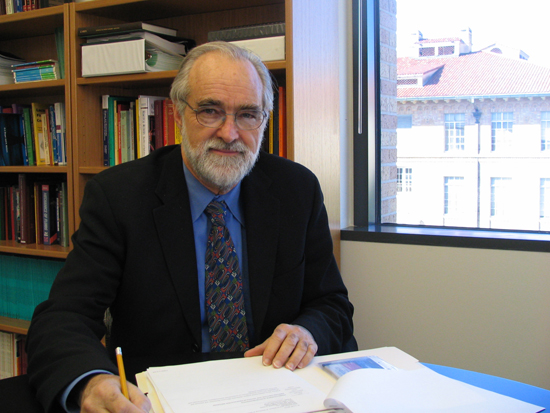
\includegraphics[width=\textwidth]{grahamcarey}
    \end{column}
  \end{columns}
}

\subsection{Background}
%%%%%%%%%%%%%%%%%%%%%%%%%%%%%%%%%%%%%%%%%%%%%%%%%
\frame
{
  \frametitle{Background}                 

  \begin{itemize}
  \item Modern simulation software is \emphcolor{complex}:
    \begin{itemize}
    \item Implicit numerical methods
    \item Massively parallel computers
    \item Adaptive methods
    \item Multiple, coupled physical processes
    \end{itemize}
    %\pause
  \item There are a host of existing software libraries that excel at treating various aspects of this complexity.
  \item Leveraging existing software whenever possible is the most efficient way to manage this complexity.

  \end{itemize}
}


 

%%%%%%%%%%%%%%%%%%%%%%%%%%%%%%%%%%%%%%%%%%%%%%%%%
\frame
{
  \frametitle{Background}                 

  \begin{itemize}
  \item Modern simulation software is \emphcolor{multidisciplinary}:
    \begin{itemize}
    \item Physical Sciences
    \item Engineering
    \item Computer Science
    \item Applied Mathematics
    \item \ldots
    \end{itemize}
  \item It is not reasonable to expect a single person to have all the necessary skills for developing \& implementing high-performance numerical algorithms on modern computing architectures.
  \item Teaming is a prerequisite for success.
  \end{itemize}
}


 

%%%%%%%%%%%%%%%%%%%%%%%%%%%%%%%%%%%%%%%%%%%%%%%%%
\frame
{
  \frametitle{Background}                 
  \begin{itemize}
    \item A large class of problems are amenable to \emphcolor{mesh based} simulation techniques.
      %% \begin{columns}[t]
      %%   \column{.5\textwidth}        
      %%   \fbox{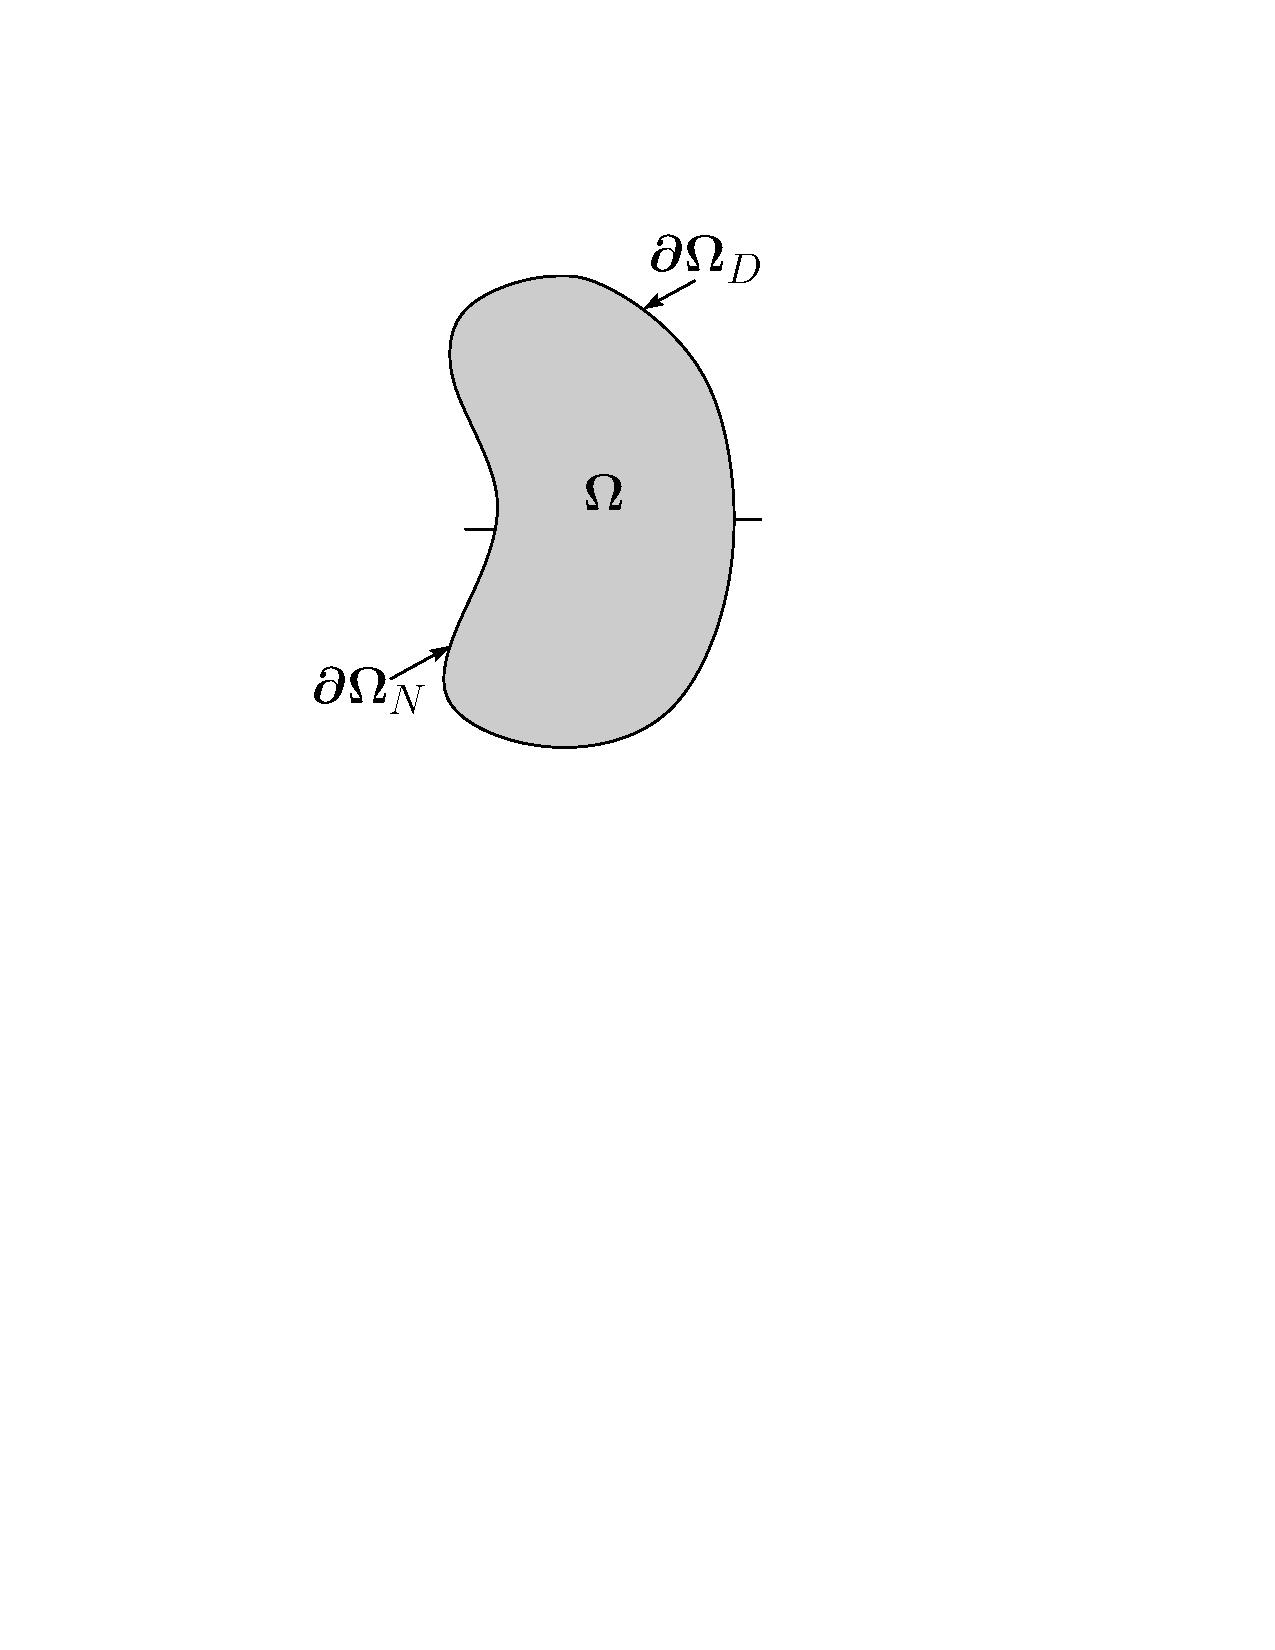
\includegraphics[viewport=140 420 400 685,clip=true,height=1in]{domain2/domain2_input}}
      %%   \column{.5\textwidth}
      %%   \fbox{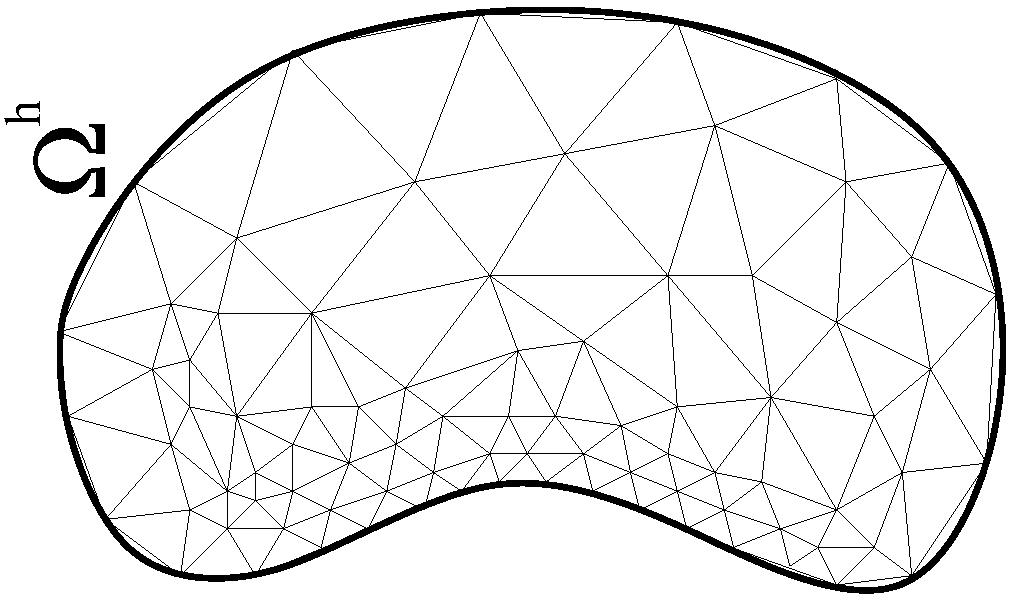
\includegraphics[height=1in,angle=-90]{discretized_domain}}
      %% \end{columns}
    \item Consider some of the major components such a simulation:
      \pause
      \begin{enumerate}
        \item Read the mesh from file
        \item Initialize data structures
        \item Construct a discrete representation of the governing equations
        \item Solve the discrete system
        \item Write out results
        \item Optionally estimate error, refine the mesh, and repeat
      \end{enumerate}

    \pause
    \item With the exception of step 3, the rest is \emph{independent} of the class of problems being solved.
    \pause
    \item This allows the major components of such a simulation to be abstracted \& implemented in a reusable software library.
  \end{itemize}
}


 

\subsection{The \libmesh{} Software Library}
%%%%%%%%%%%%%%%%%%%%%%%%%%%%%%%%%%%%%%%%%%%%%%%%%
\frame
{
  \frametitle{The \libmesh{} Software Library}
  \begin{itemize}
    \item In 2002, the \libmesh{} library began with these ideas in mind.
    \item Primary goal is to provide data structures and algorithms that can be shared by disparate physical applications, that may need some combination of
      \begin{itemize}
      \item Implicit numerical methods
      \item Adaptive mesh refinement techniques
      \item Parallel computing
      \end{itemize}
    \item Unifying theme: \emphcolor{mesh-based simulation of partial differential equations (PDEs)}.
  \end{itemize}
}



 

\subsection{Software Reusability}
%%%%%%%%%%%%%%%%%%%%%%%%%%%%%%%%%%%%%%%%%%%%%%%%%
\frame
{
  \frametitle{The \libmesh{} Software Library}

  \begin{block}{Key Point}
    \begin{itemize}
      \item The \libmesh{} library is designed to be used by students, researchers, scientists, and engineers as a tool for \emphcolor{developing simulation codes} or as a tool for \emphcolor{rapidly implementing a numerical method}.
      \item \libMesh{} is not an application code.
      \item It does not ``solve problem XYZ.''
        \begin{itemize}
          \item It can be used to help you develop an application to solve problem XYZ, and to do so quickly with advanced numerical algorithms on high-performance computing platforms.
        \end{itemize}
      %\item It was initially targeted for finite element based simulations, but has been used for finite volume discretizations as well.
    \end{itemize}    
  \end{block}
} 



%%%%%%%%%%%%%%%%%%%%%%%%%%%%%%%%%%%%%%%%%%%%%%%%%
\frame
{
  \frametitle{Software Reusability}
  \begin{itemize}
    \item At the inception of \libMesh{} in 2002, there were many high-quality software libraries that implemented some aspect of the end-to-end PDE simulation process:
      \begin{itemize}
        \item Parallel linear algebra
        \item Partitioning algorithms for domain decomposition
        \item Visualization formats
        \item \ldots
      \end{itemize}
    \item A design goal of \libMesh{} has always been to provide flexible \& extensible interfaces to existing software whenever possible.
    \item We implement the ``glue'' to these pieces, as well as what we viewed as the missing infrastructure:
      \begin{itemize}
        \item \emphcolor{Flexible data structures for the discretization of spatial domains and systems of PDEs posed on these domains.}
      \end{itemize}          
  \end{itemize}  
}



%%%%%%%%%%%%%%%%%%%%%%%%%%%%%%%%%%%%%%%%%%%%%%%%%
\begin{frame}[t]
  %\frametitle{LibMesh Tree}
%  \vspace{-.25in}
%  \begin{center}
%    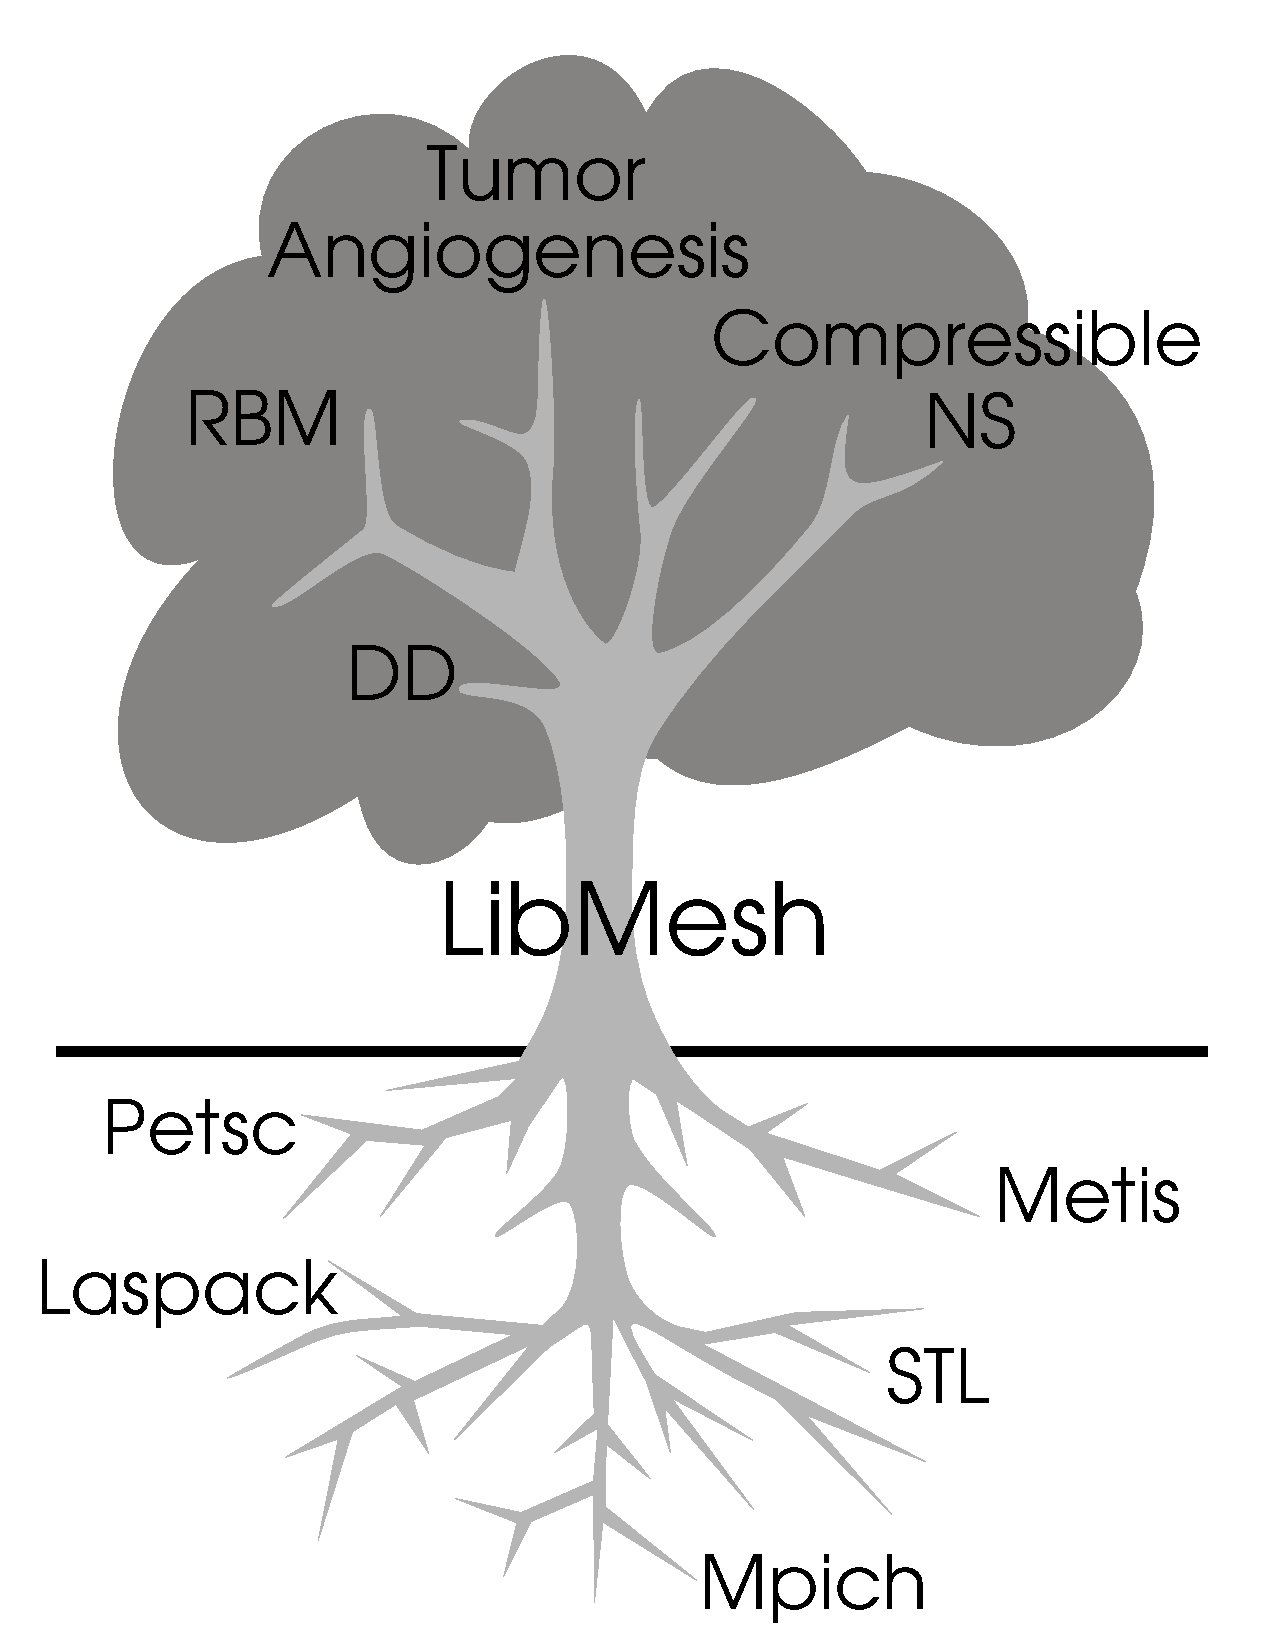
\includegraphics[width=.6\textwidth]{mytreeandroots_allnames}    
%  \end{center}


    \begin{minipage}[h]{.6\textwidth}
    \begin{center}
      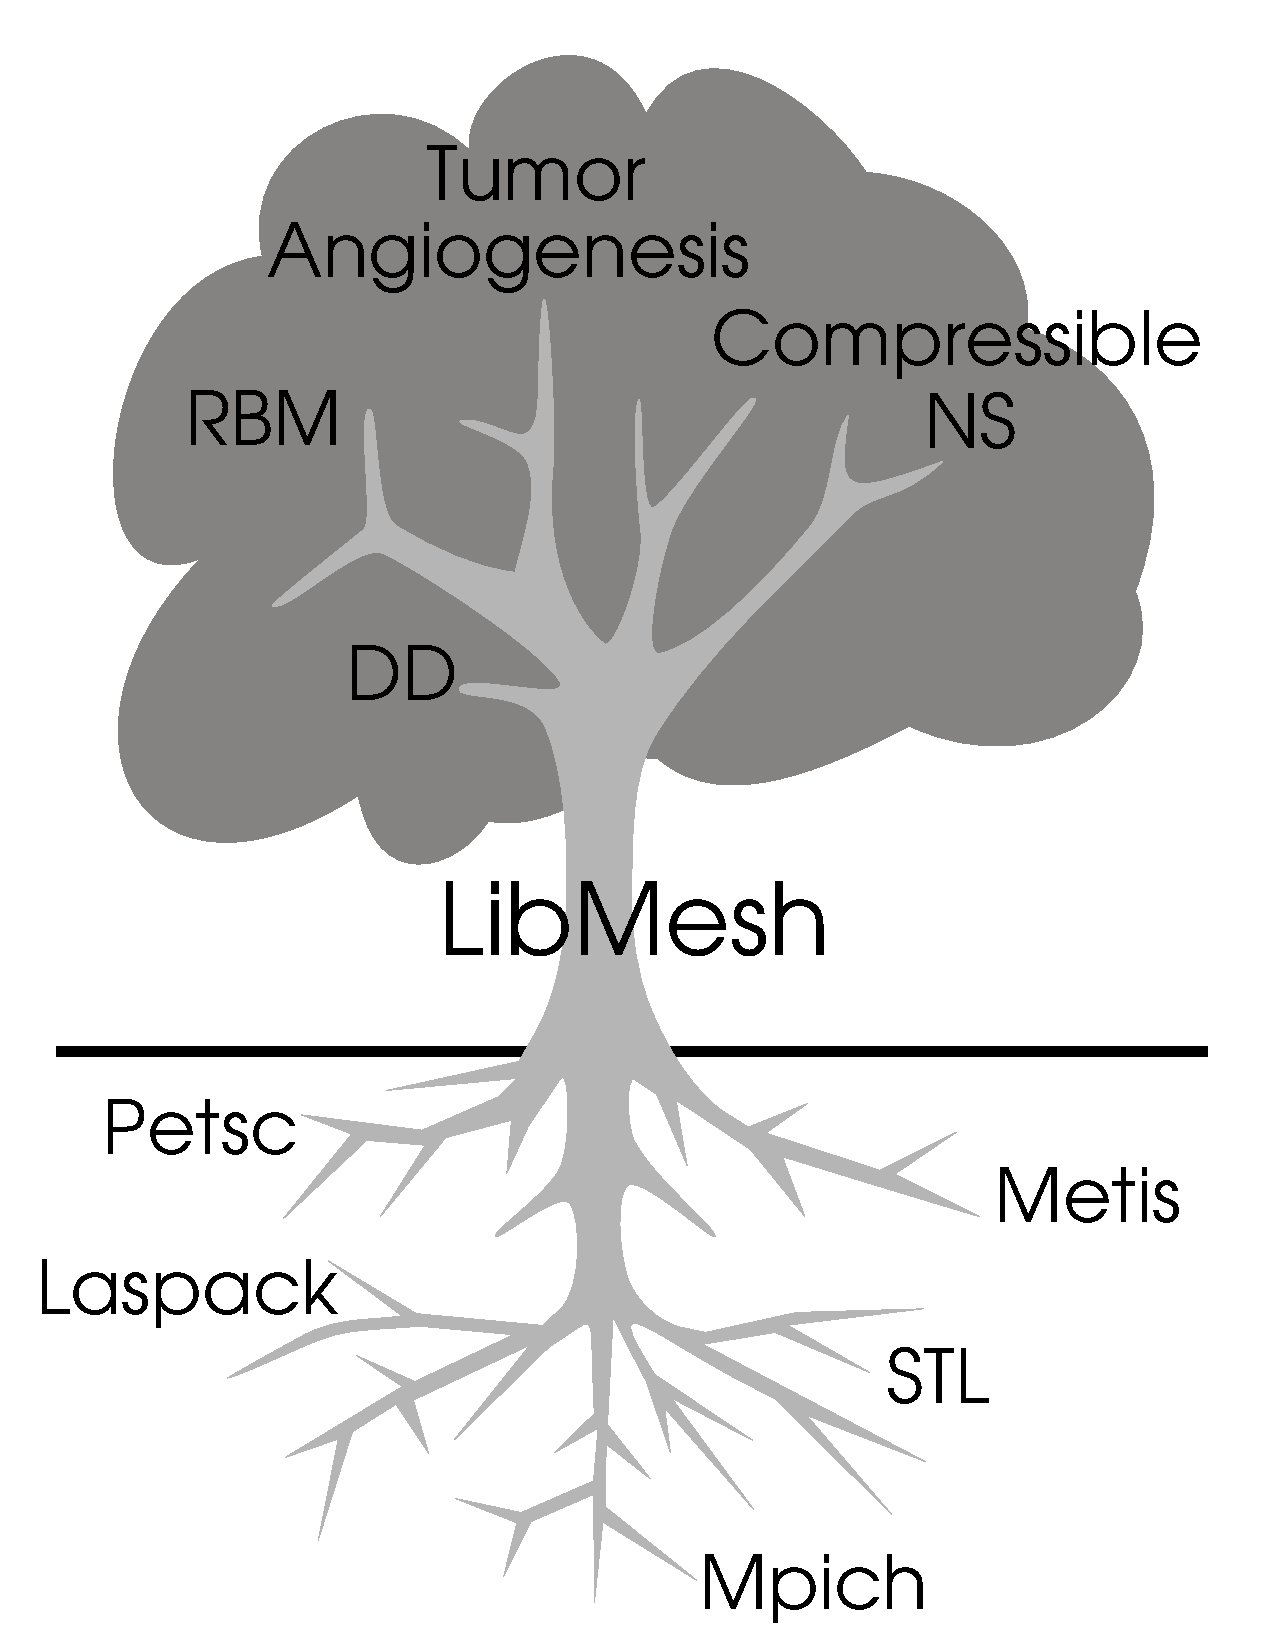
\includegraphics[width=.9\textwidth]{mytreeandroots_allnames}
    \end{center}
  \end{minipage}
  \begin{minipage}[h]{.35\textwidth}
    \begin{block}{Library Structure}
      \begin{itemize}
        %\small
    \item Basic libraries are \LibMesh's ``roots''
    \item Application ``branches'' built off the library ``trunk''
      \end{itemize}
    \end{block}
  \end{minipage}
\end{frame}


\subsection{Library Trivia}
\frame
{
  \frametitle{Trivia -- Downloads}
  \begin{center}
    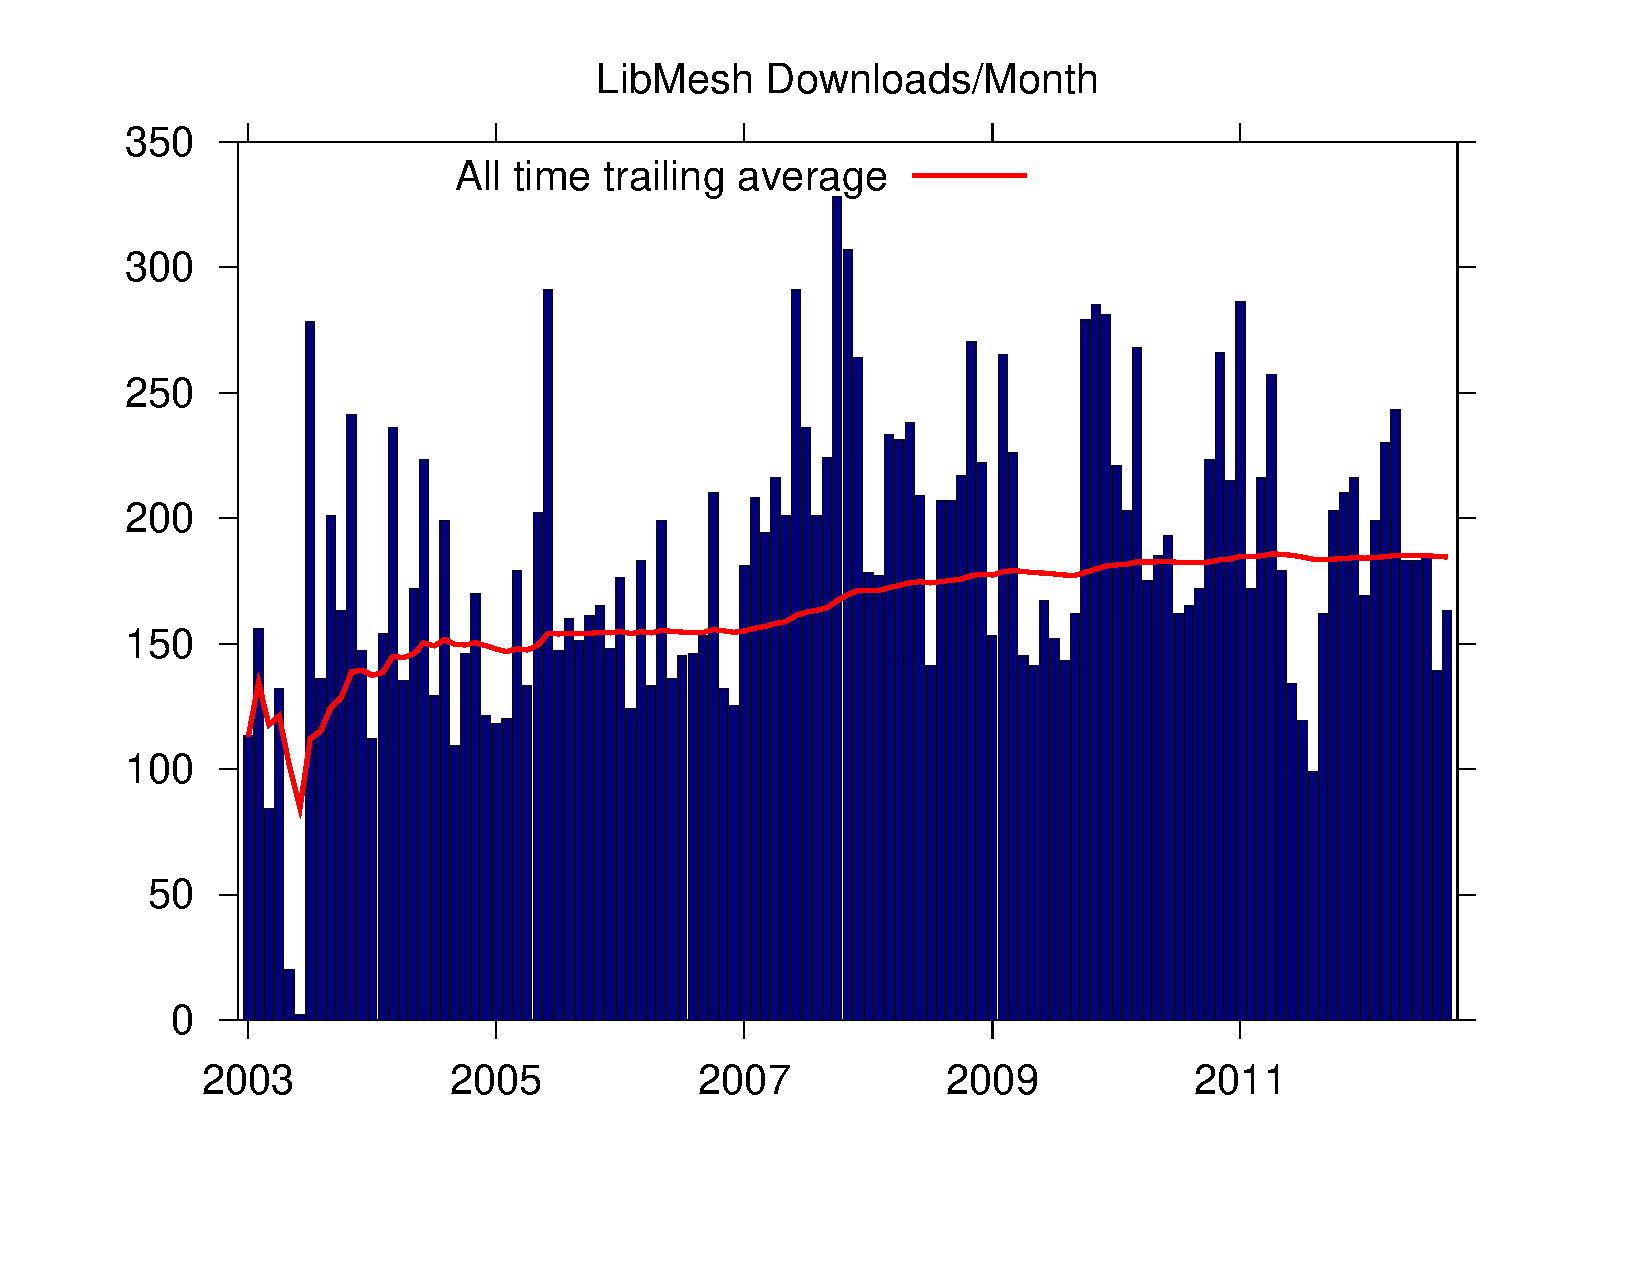
\includegraphics[height=0.8\textheight]{trivia/libmesh_downloads}
  \end{center}
}       

\frame
{
  \frametitle{Trivia -- Mailing List Membership}
  \begin{center}
    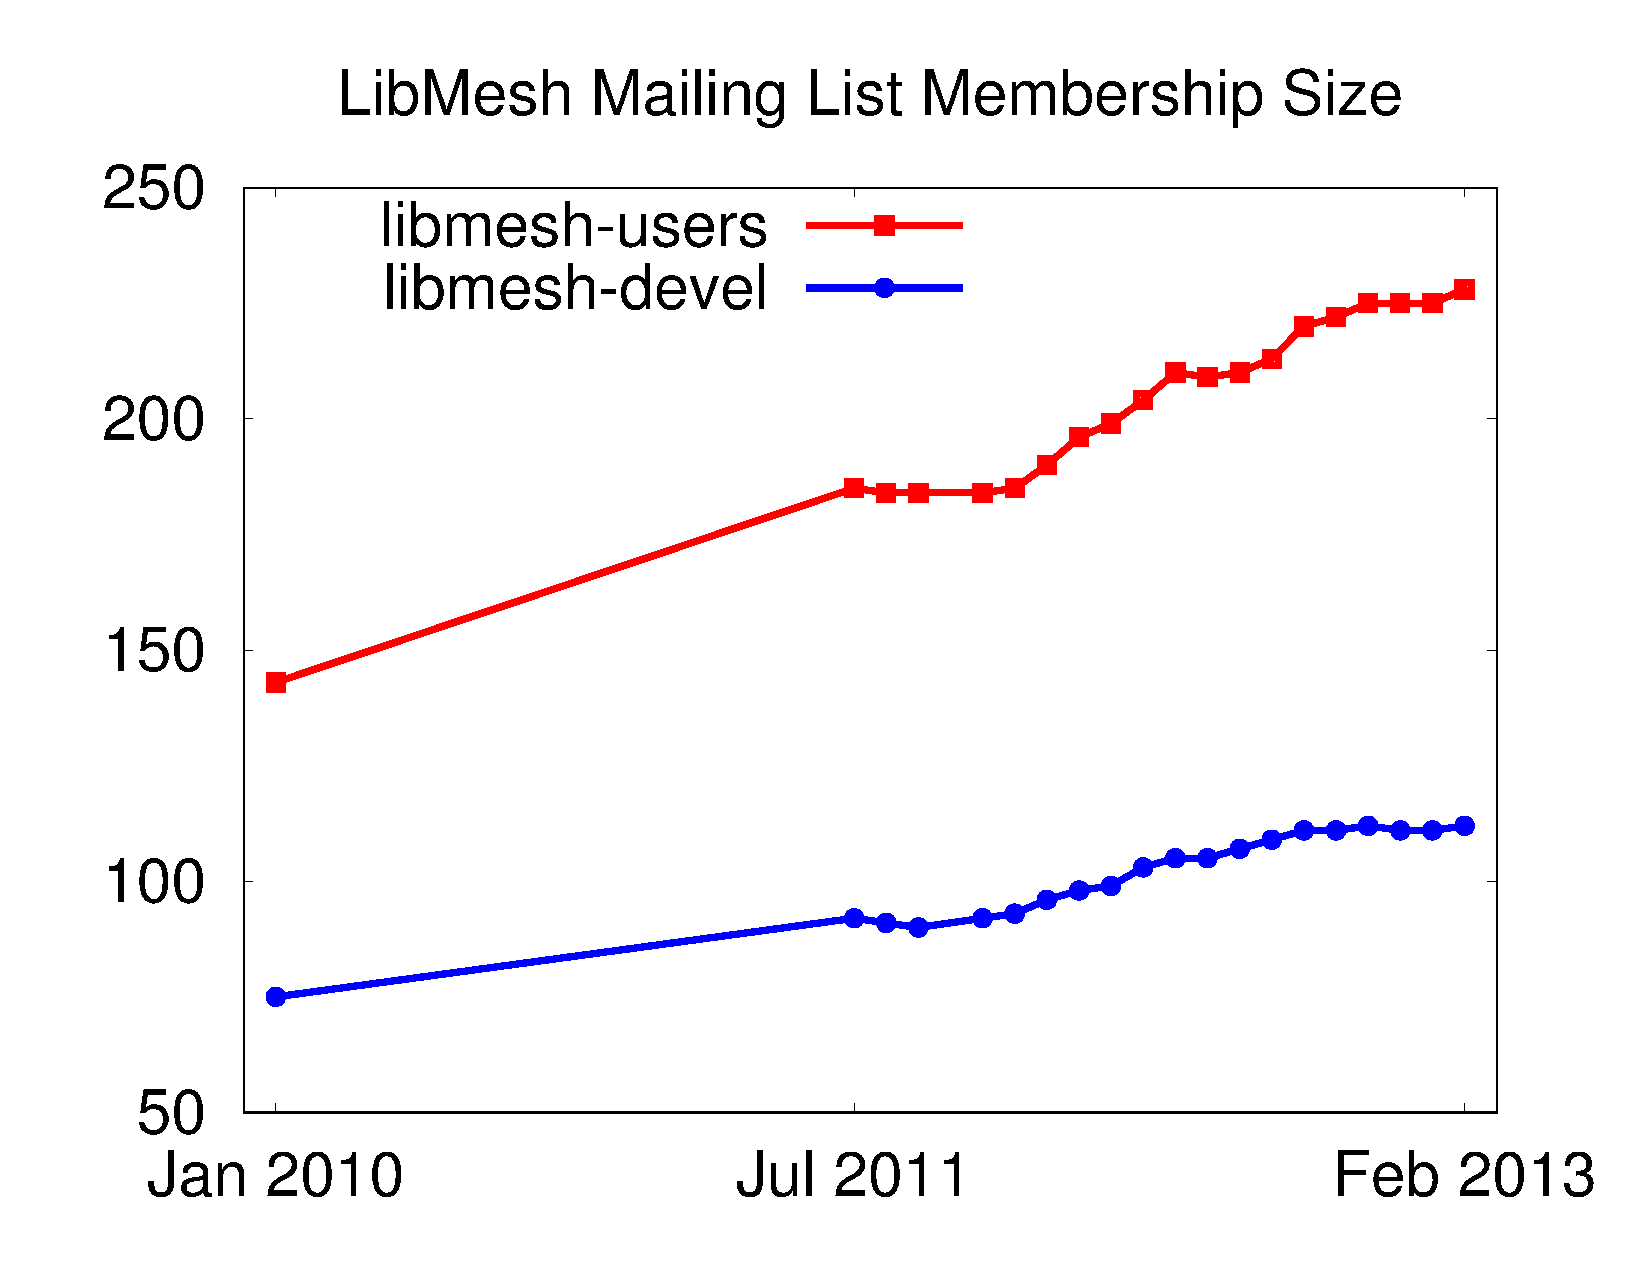
\includegraphics[height=0.8\textheight]{trivia/libmesh_mailinglists_membership}
    
    \small
    
    \url{libmesh-users@lists.sourceforge.net}

    \url{libmesh-devel@lists.sourceforge.net}
  \end{center}
}       

\frame
{
  \frametitle{Trivia -- Citations}
  \begin{center}
    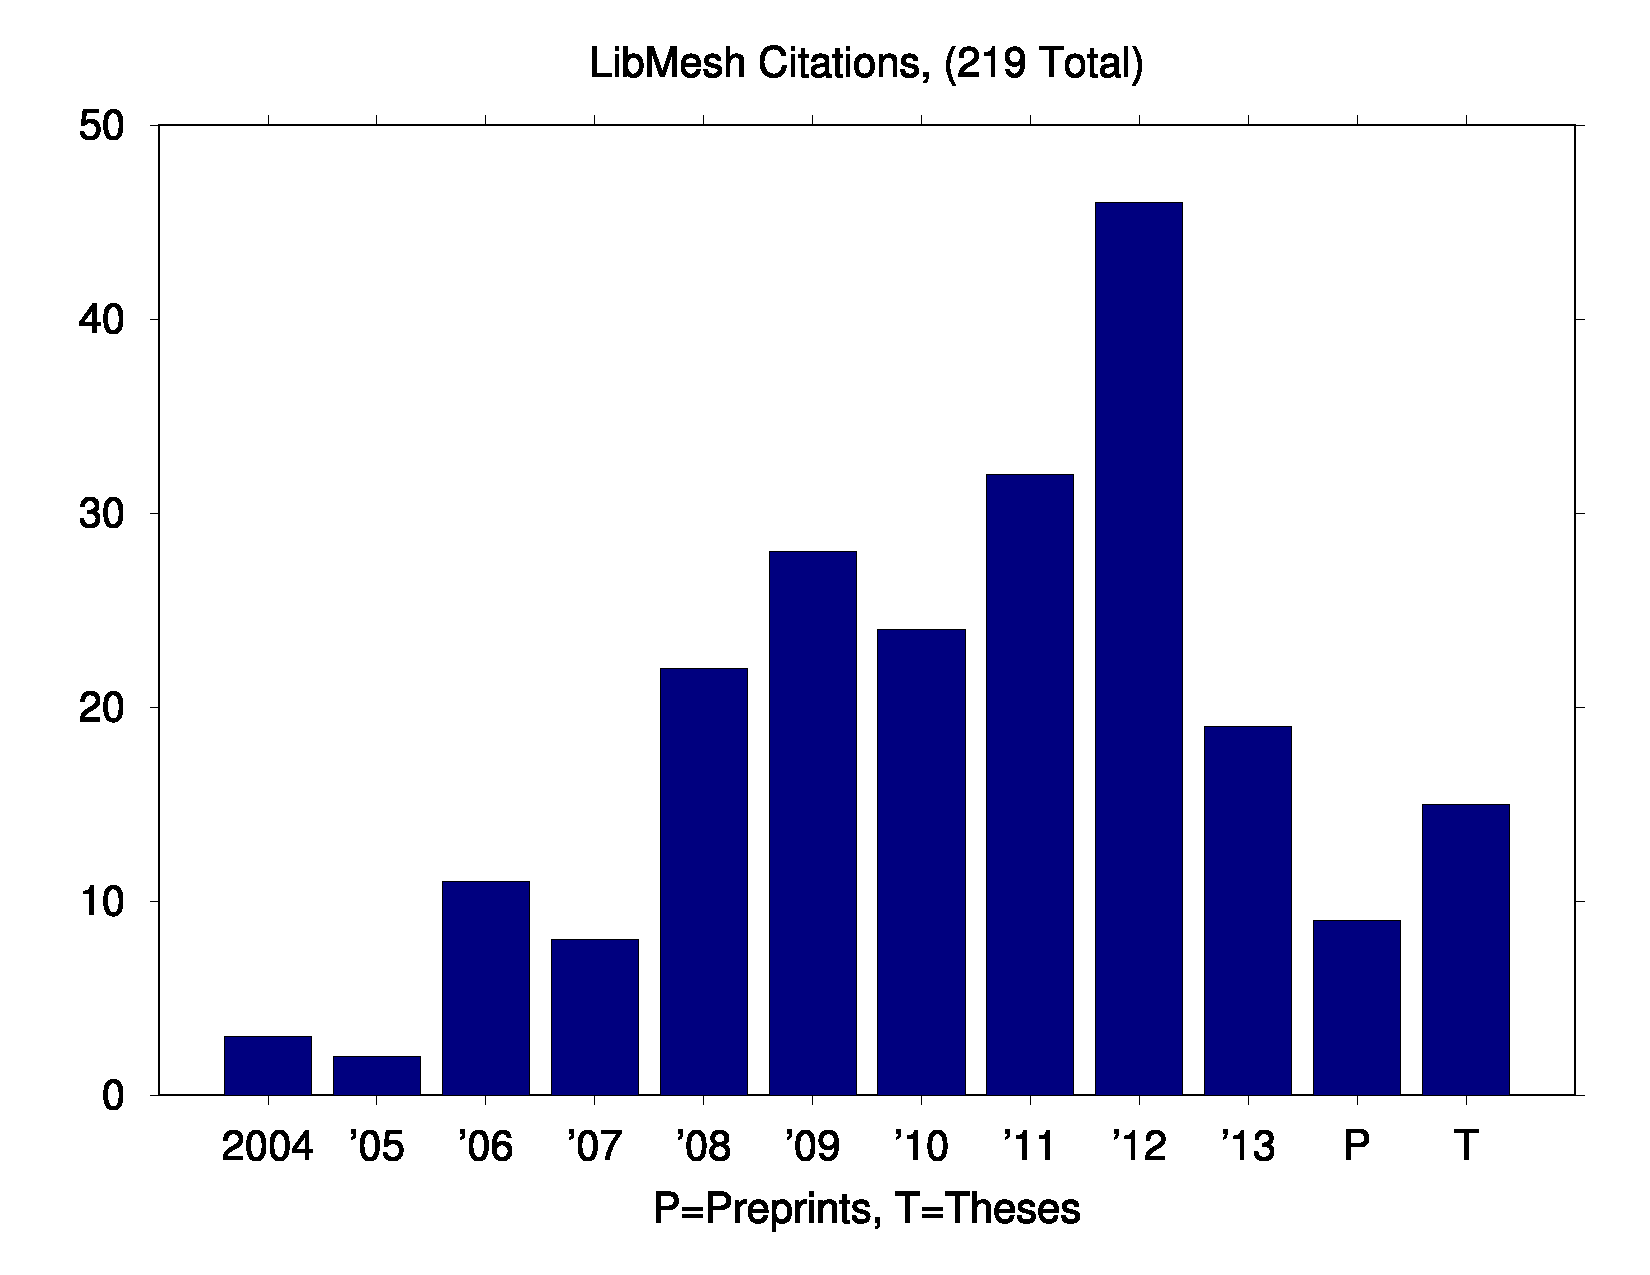
\includegraphics[height=0.8\textheight]{trivia/libmesh_citations}
  \end{center}
}       


\subsection{Library Design}
%%%%%%%%%%%%%%%%%%%%%%%%%%%%%%%%%%%%%%%%%%%%%%%%%
\frame
{
  \frametitle{The ``Glue''}
  \begin{itemize}
    \item The \cpp{} programming language provides a powerful abstraction mechanism for separating a software interface from its implementation.
    \item The notion of \emphcolor{Base Classes} defining an abstract interface and \emphcolor{Derived Classes} implementing the interface is key to this programming model.
      \pause
    \item The classic \cpp{} example: Shapes.
  \end{itemize}
  \lstinputlisting{snippets/shapes/main.cxx}
}



%%%%%%%%%%%%%%%%%%%%%%%%%%%%%%%%%%%%%%%%%%%%%%%%%
\frame
{
  \frametitle{Abstract Shape}
  \lstinputlisting{snippets/shapes/shape.cxx}
}



%%%%%%%%%%%%%%%%%%%%%%%%%%%%%%%%%%%%%%%%%%%%%%%%%
\frame
{
  \frametitle{Specific Shape: Rectangle}
  \lstinputlisting{snippets/shapes/rectangle.cxx}
}



%%%%%%%%%%%%%%%%%%%%%%%%%%%%%%%%%%%%%%%%%%%%%%%%%
\frame
{
  \frametitle{Specific Shape: Circle}
  \lstinputlisting{snippets/shapes/circle.cxx}
}



%%%%%%%%%%%%%%%%%%%%%%%%%%%%%%%%%%%%%%%%%%%%%%%%%
\frame
{
  \frametitle{Object Polymorphism}
  \lstinputlisting{snippets/shapes/main2.cxx}
}



%%%%%%%%%%%%%%%%%%%%%%%%%%%%%%%%%%%%%%%%%%%%%%%%%
\frame
{
  \Large
  \begin{block}{}
    \center{Examples of Polymorphism in}
    \center{\bf \libmesh{}}
  \end{block}
}



%%%%%%%%%%%%%%%%%%%%%%%%%%%%%%%%%%%%%%%%%%%%%%%%%
\frame
{
  \frametitle{The ``Glue:'' Linear Algebra}
  \begin{center}
    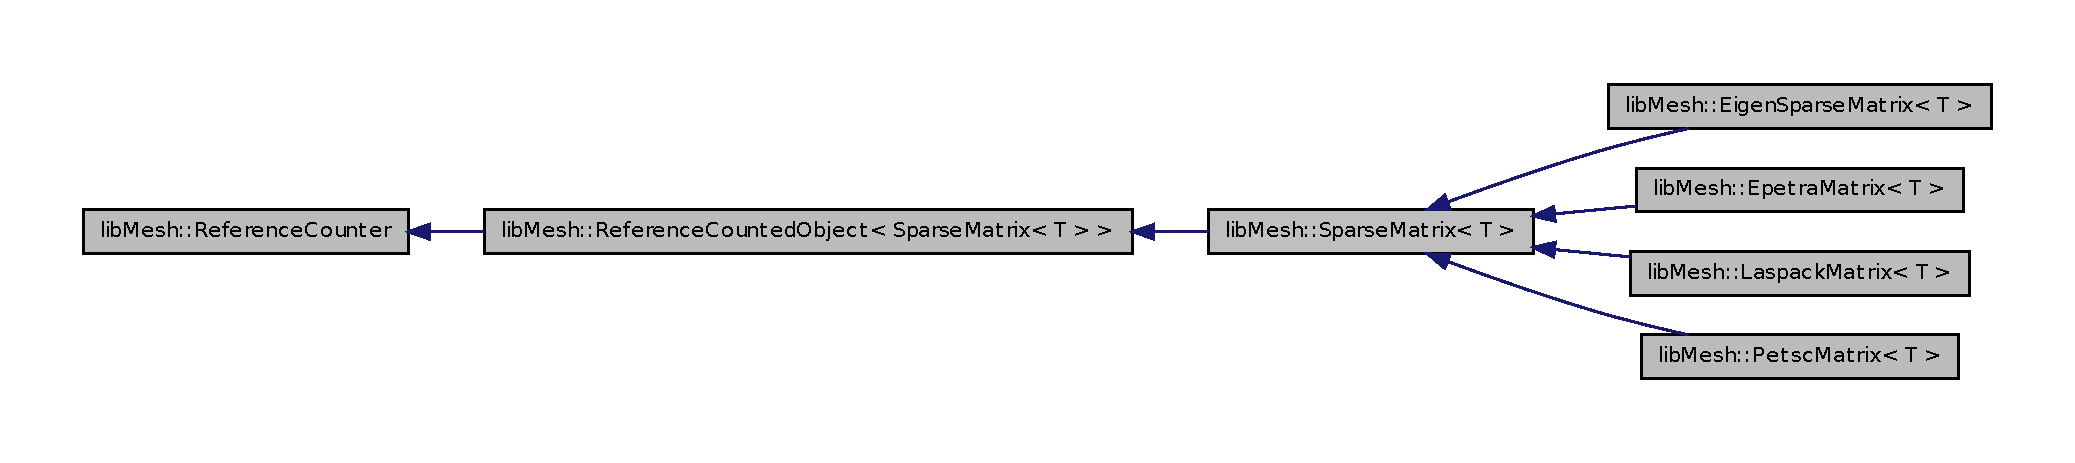
\includegraphics[width=\textwidth,trim=7.56in 0 0 0,clip]{libmesh_docs/classlibMesh_1_1SparseMatrix__inherit__graph}
  \end{center}
}



%%%%%%%%%%%%%%%%%%%%%%%%%%%%%%%%%%%%%%%%%%%%%%%%%
\frame
{
  \frametitle{The ``Glue:'' I/O formats}
  \begin{center}
    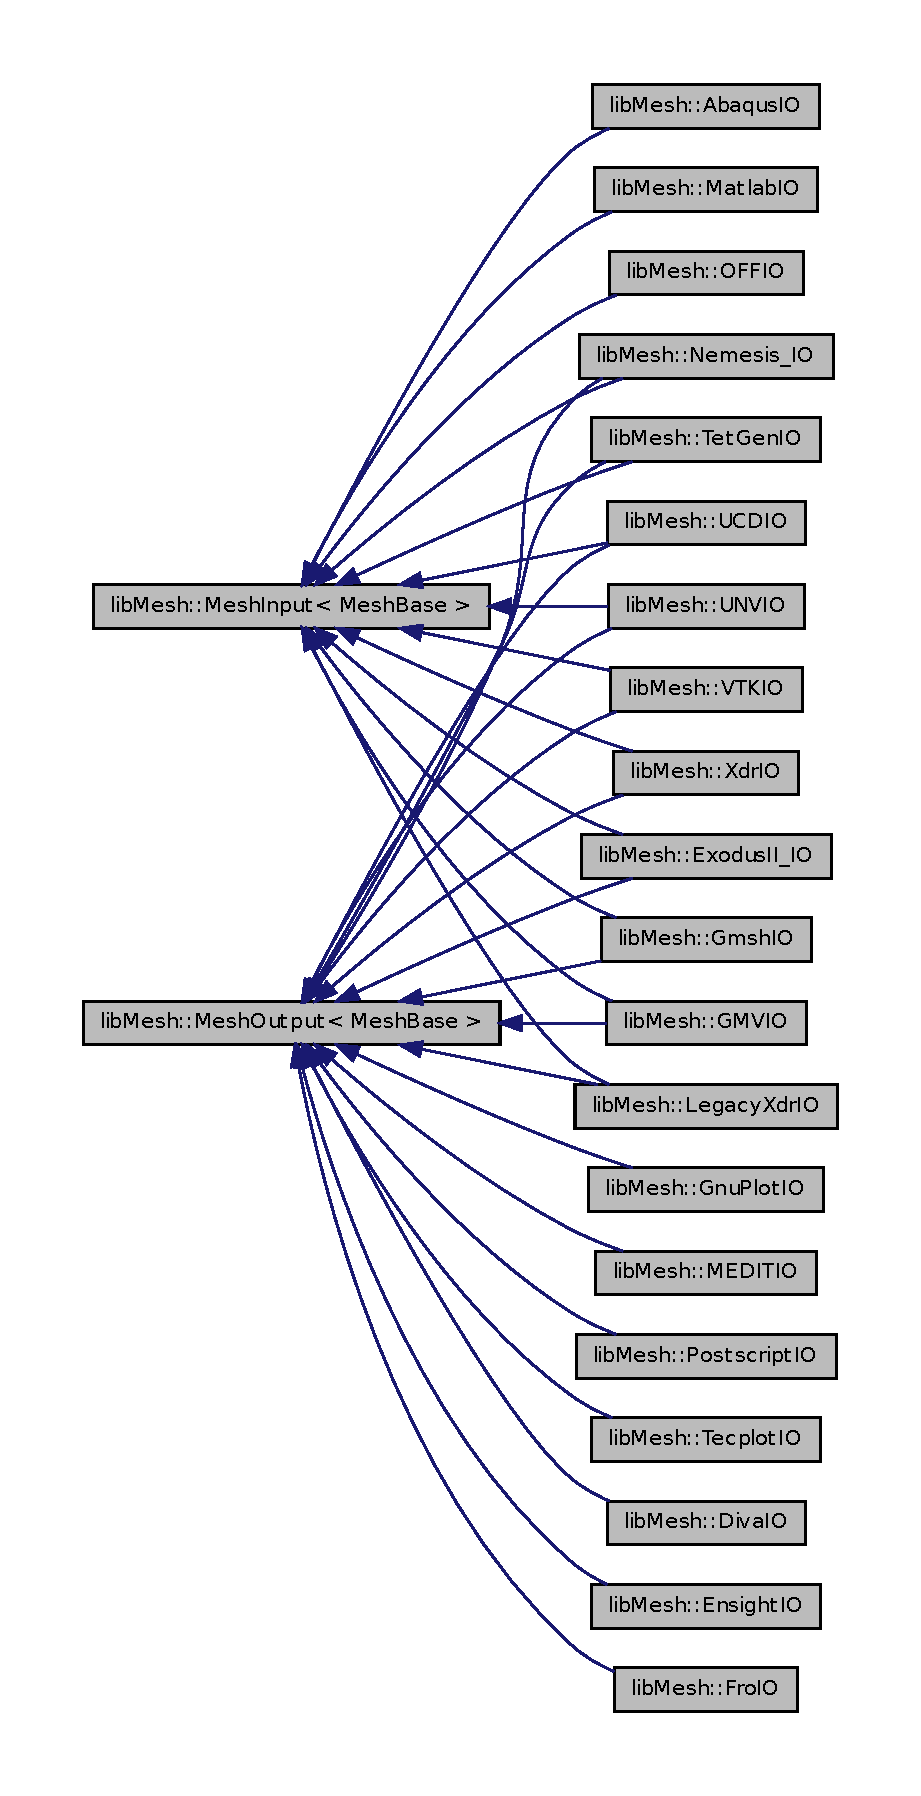
\includegraphics[height=0.9\textheight]{libmesh_docs/mesh_io}
  \end{center}
}



%%%%%%%%%%%%%%%%%%%%%%%%%%%%%%%%%%%%%%%%%%%%%%%%%
\frame
{
  \frametitle{Disretization: The Mesh}
  \begin{center}
    \includegraphics[width=\textwidth]{libmesh_docs/mesh_base}
  \end{center}
}      



%%%%%%%%%%%%%%%%%%%%%%%%%%%%%%%%%%%%%%%%%%%%%%%%%
\frame
{
  \frametitle{Disretization: Geometric Elements}
  \begin{center}
    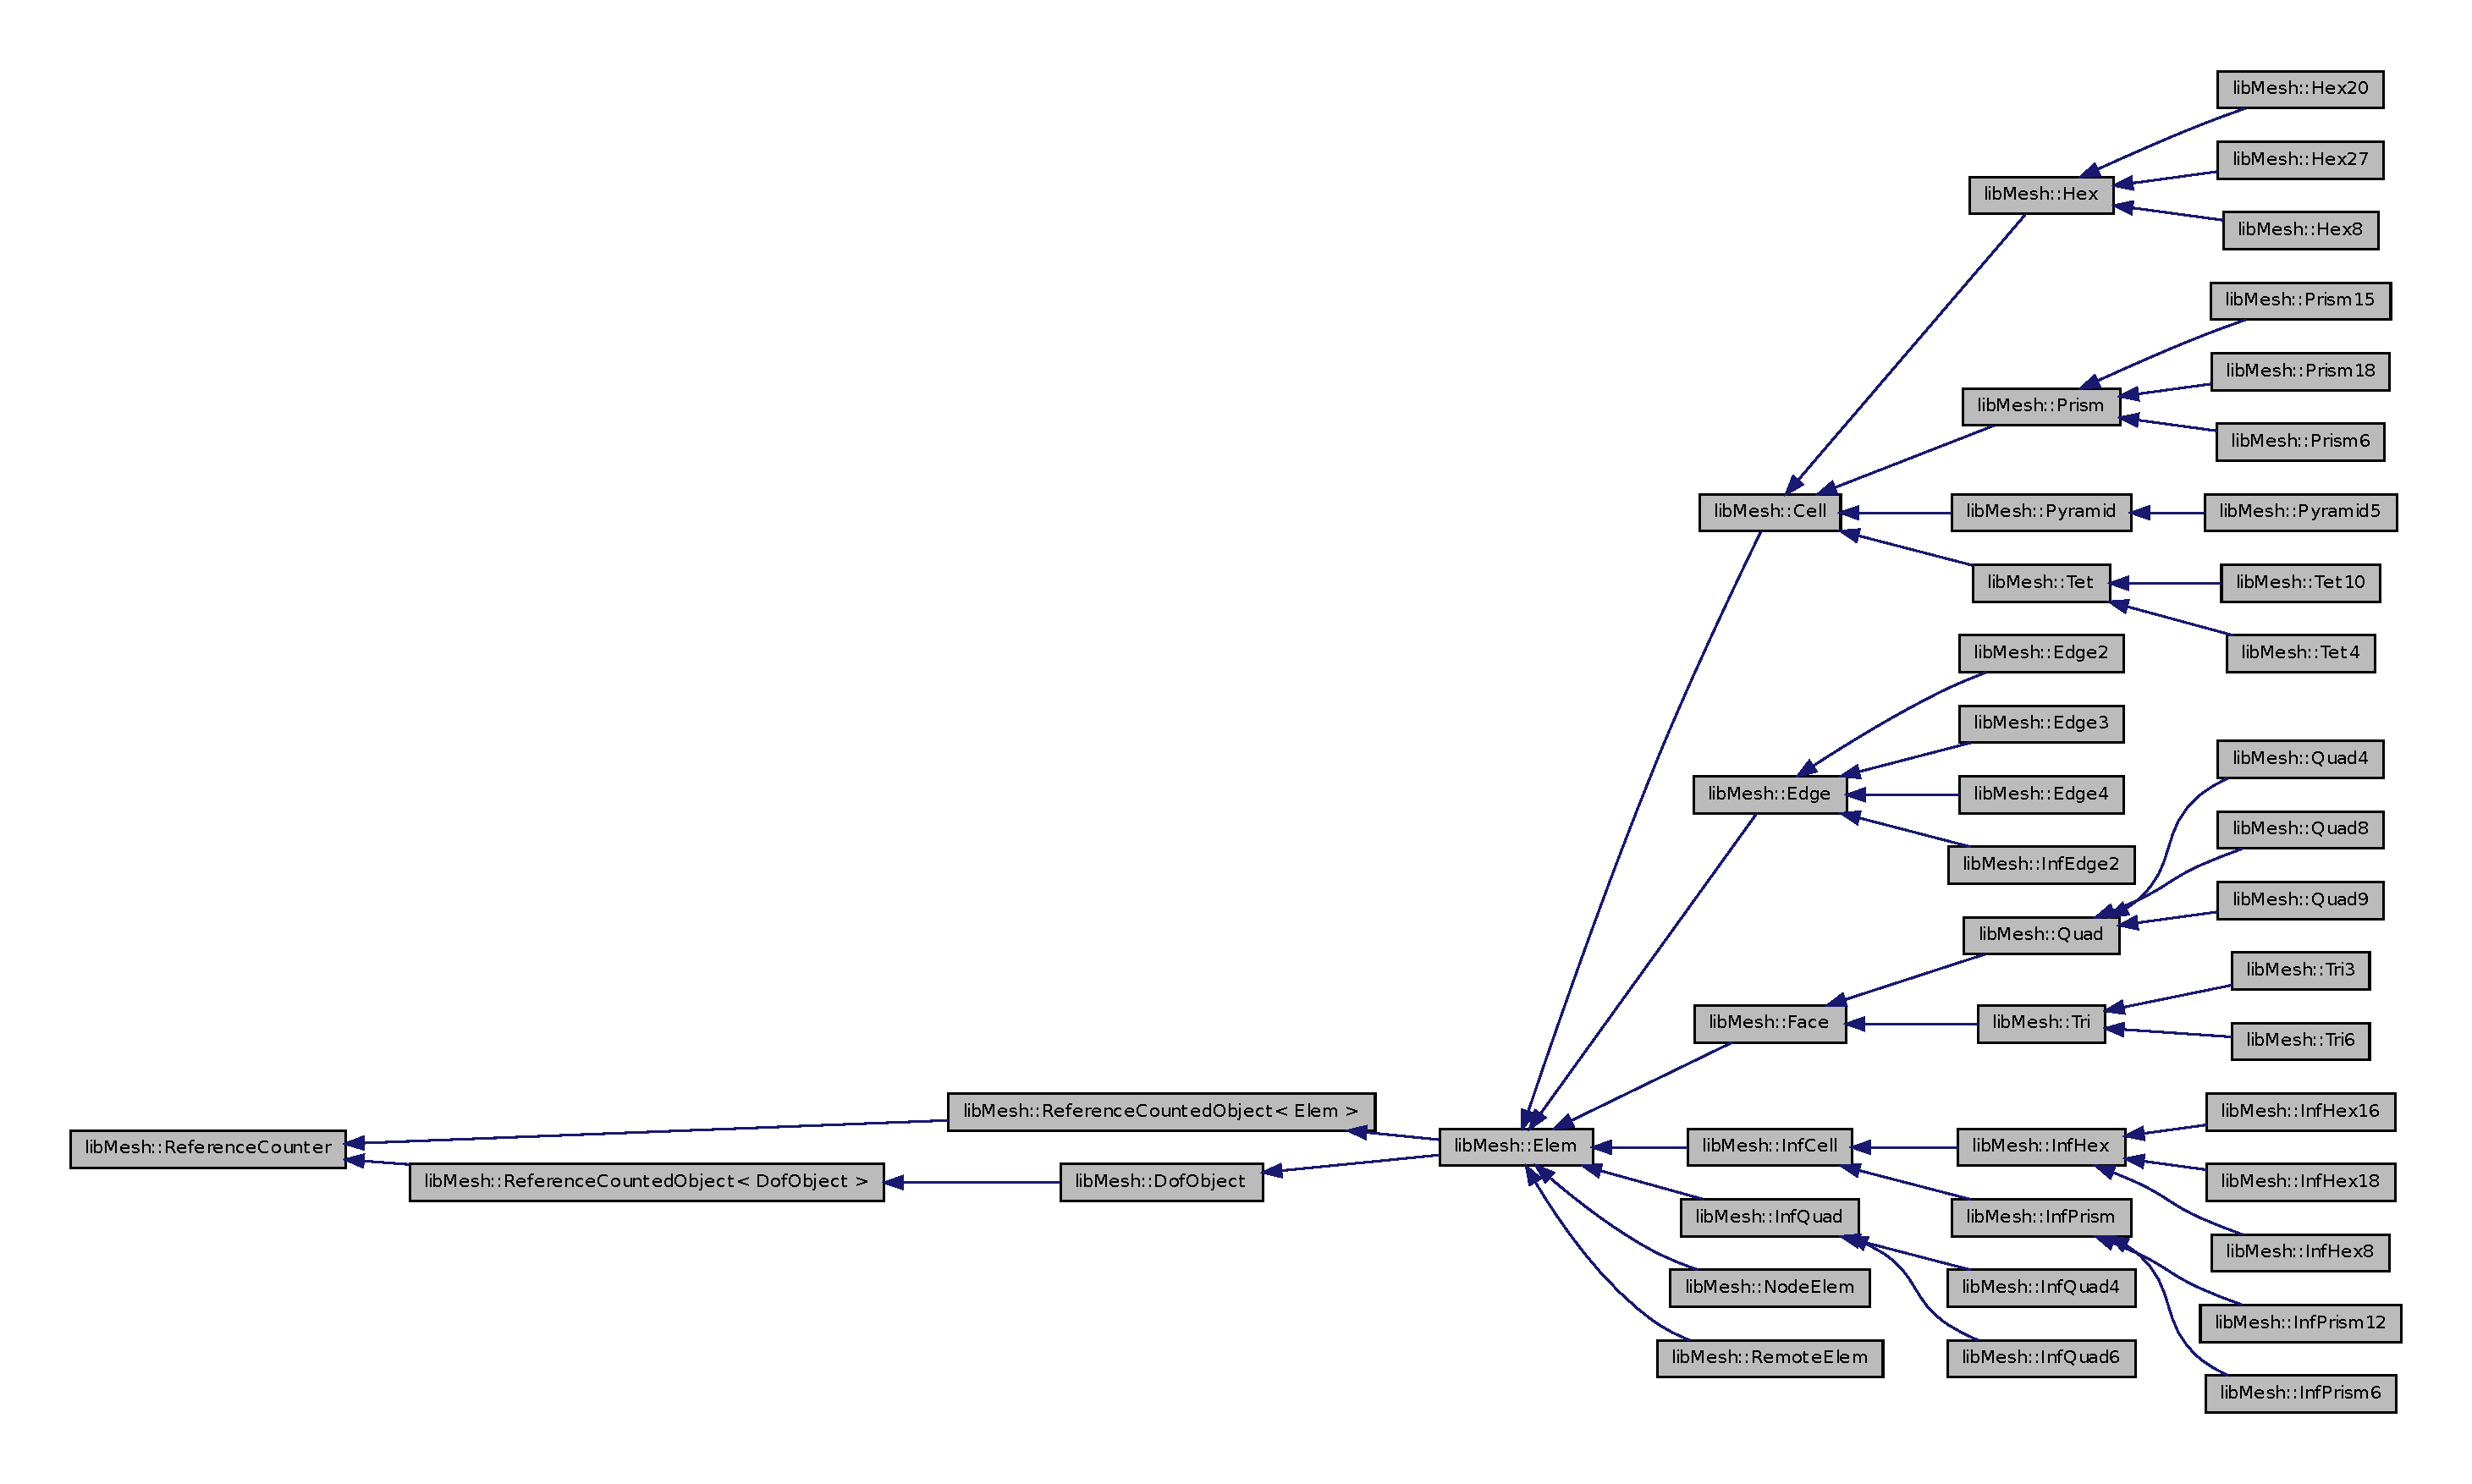
\includegraphics[width=\textwidth]{libmesh_docs/classlibMesh_1_1Elem__inherit__graph}
  \end{center}
}      



%%%%%%%%%%%%%%%%%%%%%%%%%%%%%%%%%%%%%%%%%%%%%%%%%
\frame
{
  \frametitle{Disretization: Geometric Elements}
  \begin{center}
    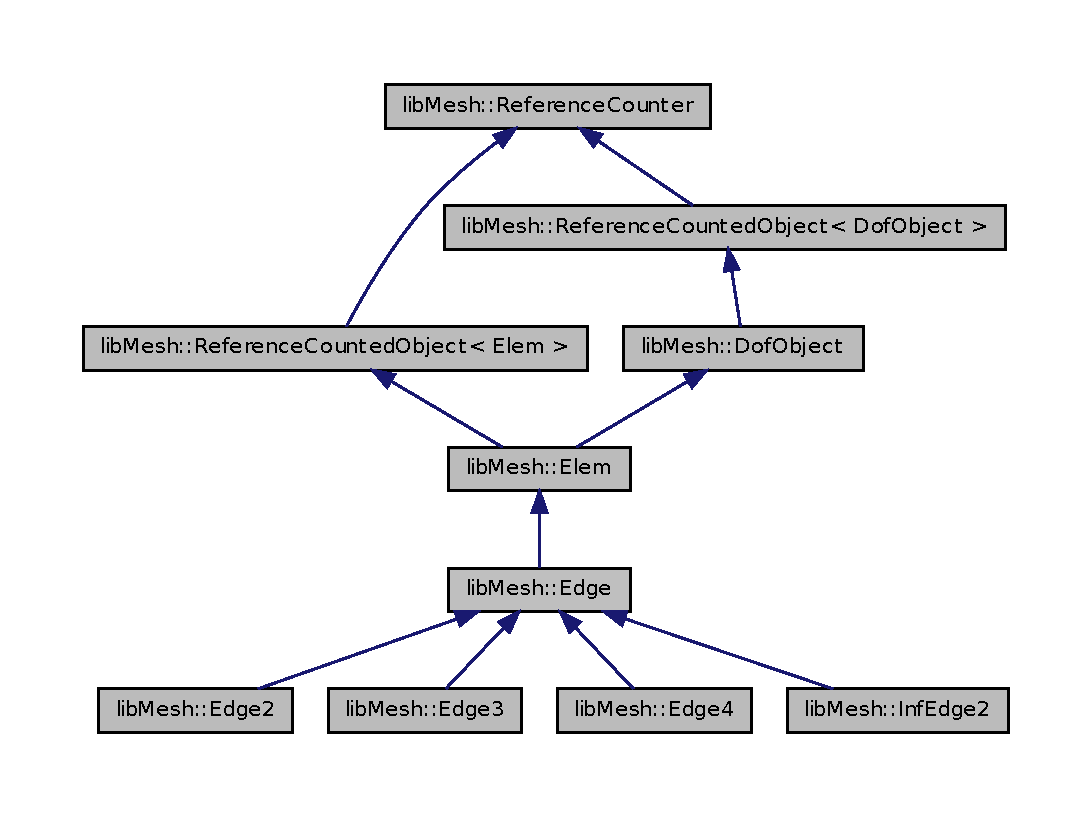
\includegraphics[width=0.9\textwidth]{libmesh_docs/classlibMesh_1_1Edge__inherit__graph}
  \end{center}
}      



%%%%%%%%%%%%%%%%%%%%%%%%%%%%%%%%%%%%%%%%%%%%%%%%%
\frame
{
  \frametitle{Disretization: Geometric Elements}
  \begin{center}
    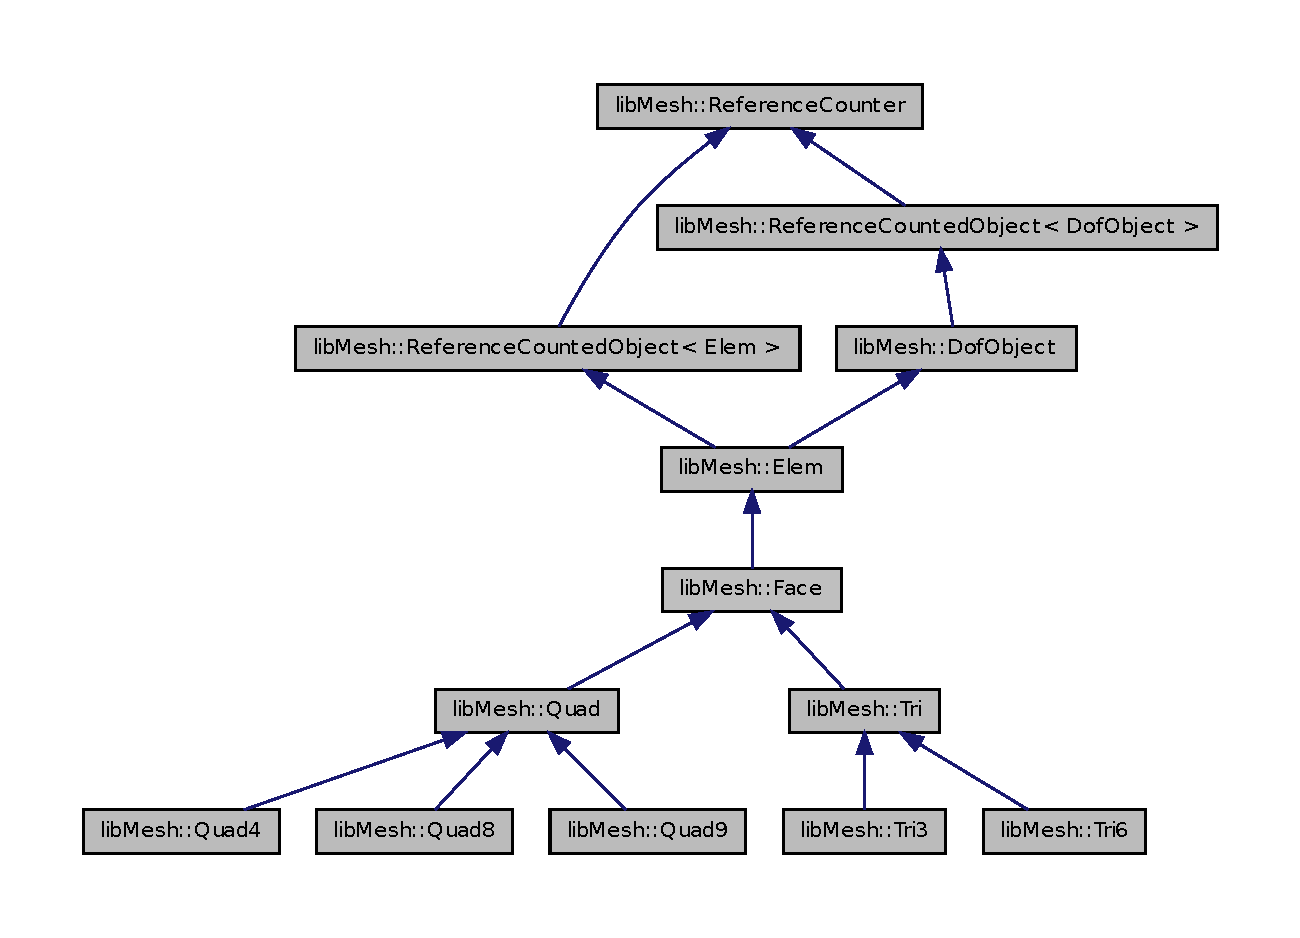
\includegraphics[width=0.95\textwidth]{libmesh_docs/classlibMesh_1_1Face__inherit__graph}
  \end{center}
}      



%%%%%%%%%%%%%%%%%%%%%%%%%%%%%%%%%%%%%%%%%%%%%%%%%
\frame
{
  \frametitle{Disretization: Geometric Elements}
  \begin{center}
    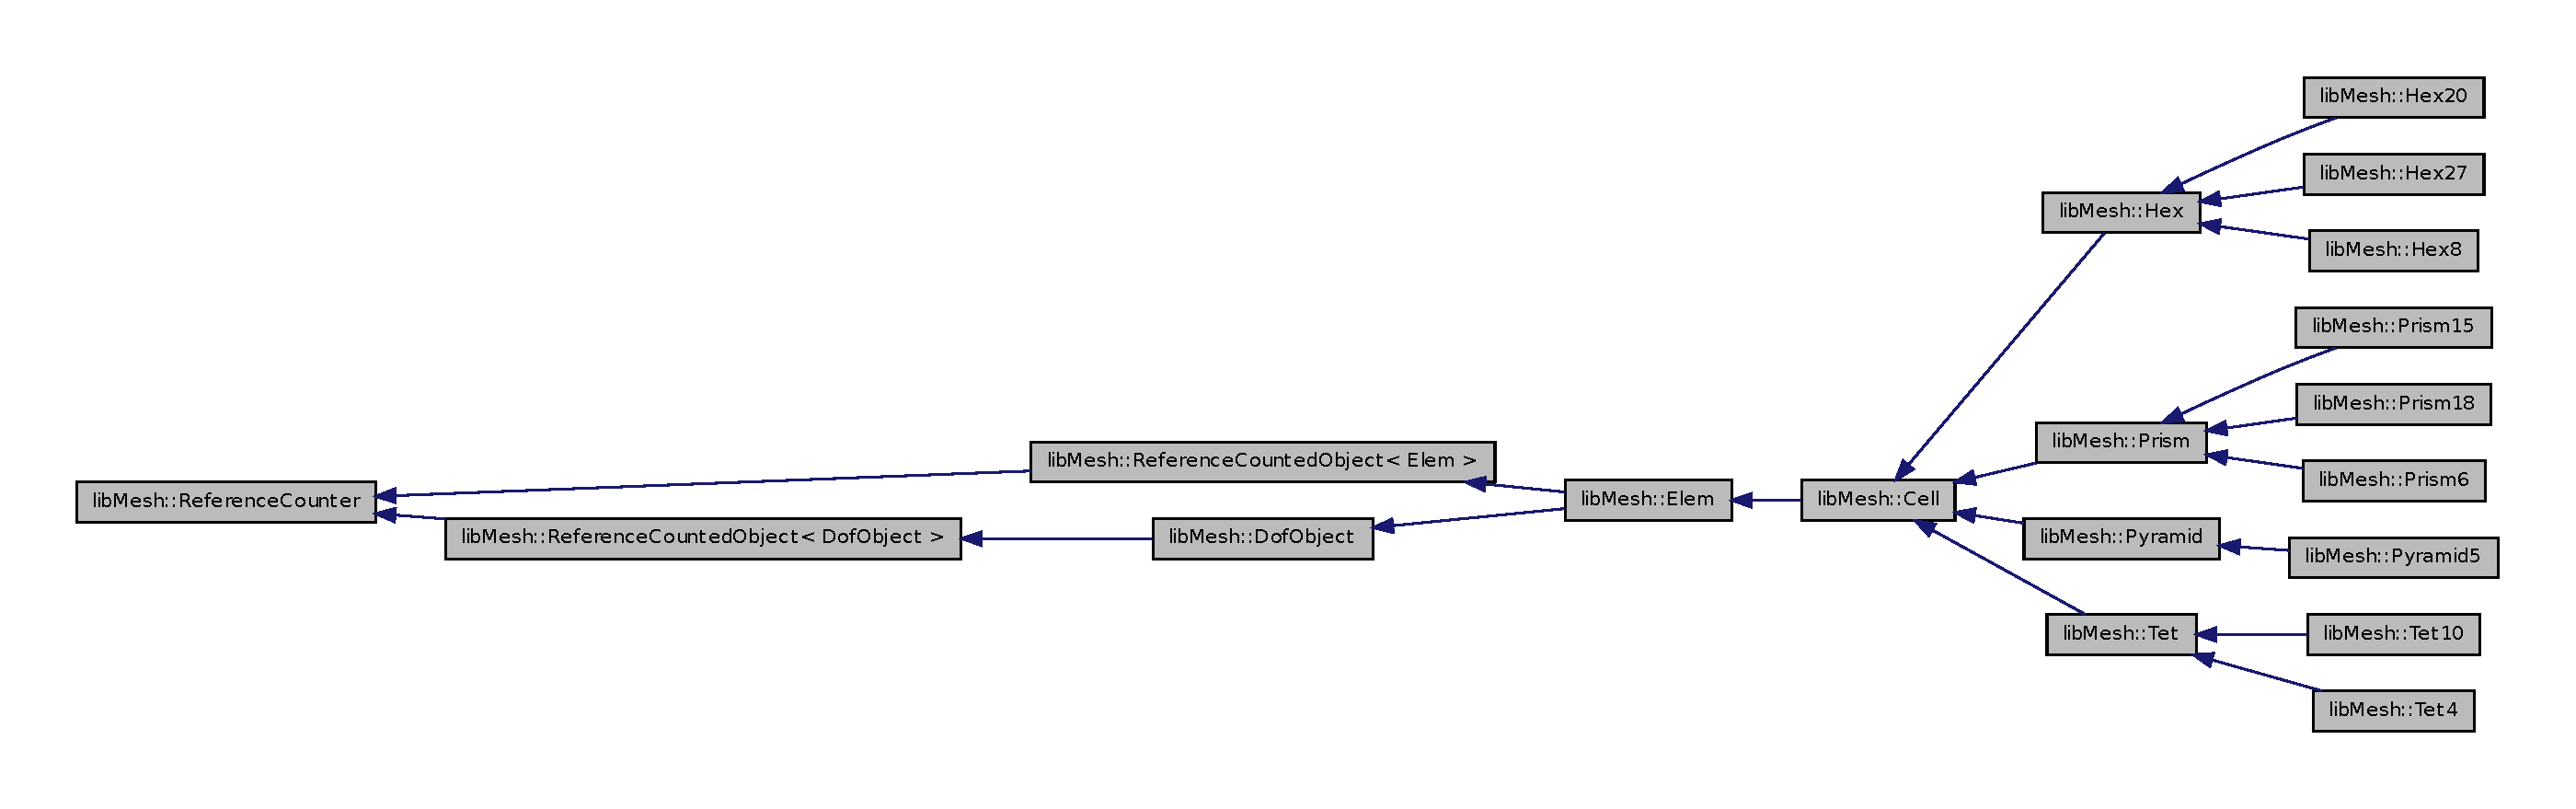
\includegraphics[width=0.9\textwidth,trim=11.3in 0 0 0,clip]{libmesh_docs/classlibMesh_1_1Cell__inherit__graph}
  \end{center}
}      



%%%%%%%%%%%%%%%%%%%%%%%%%%%%%%%%%%%%%%%%%%%%%%%%%
\frame
{
  \frametitle{Disretization: Finite Elements}
  \begin{center}
    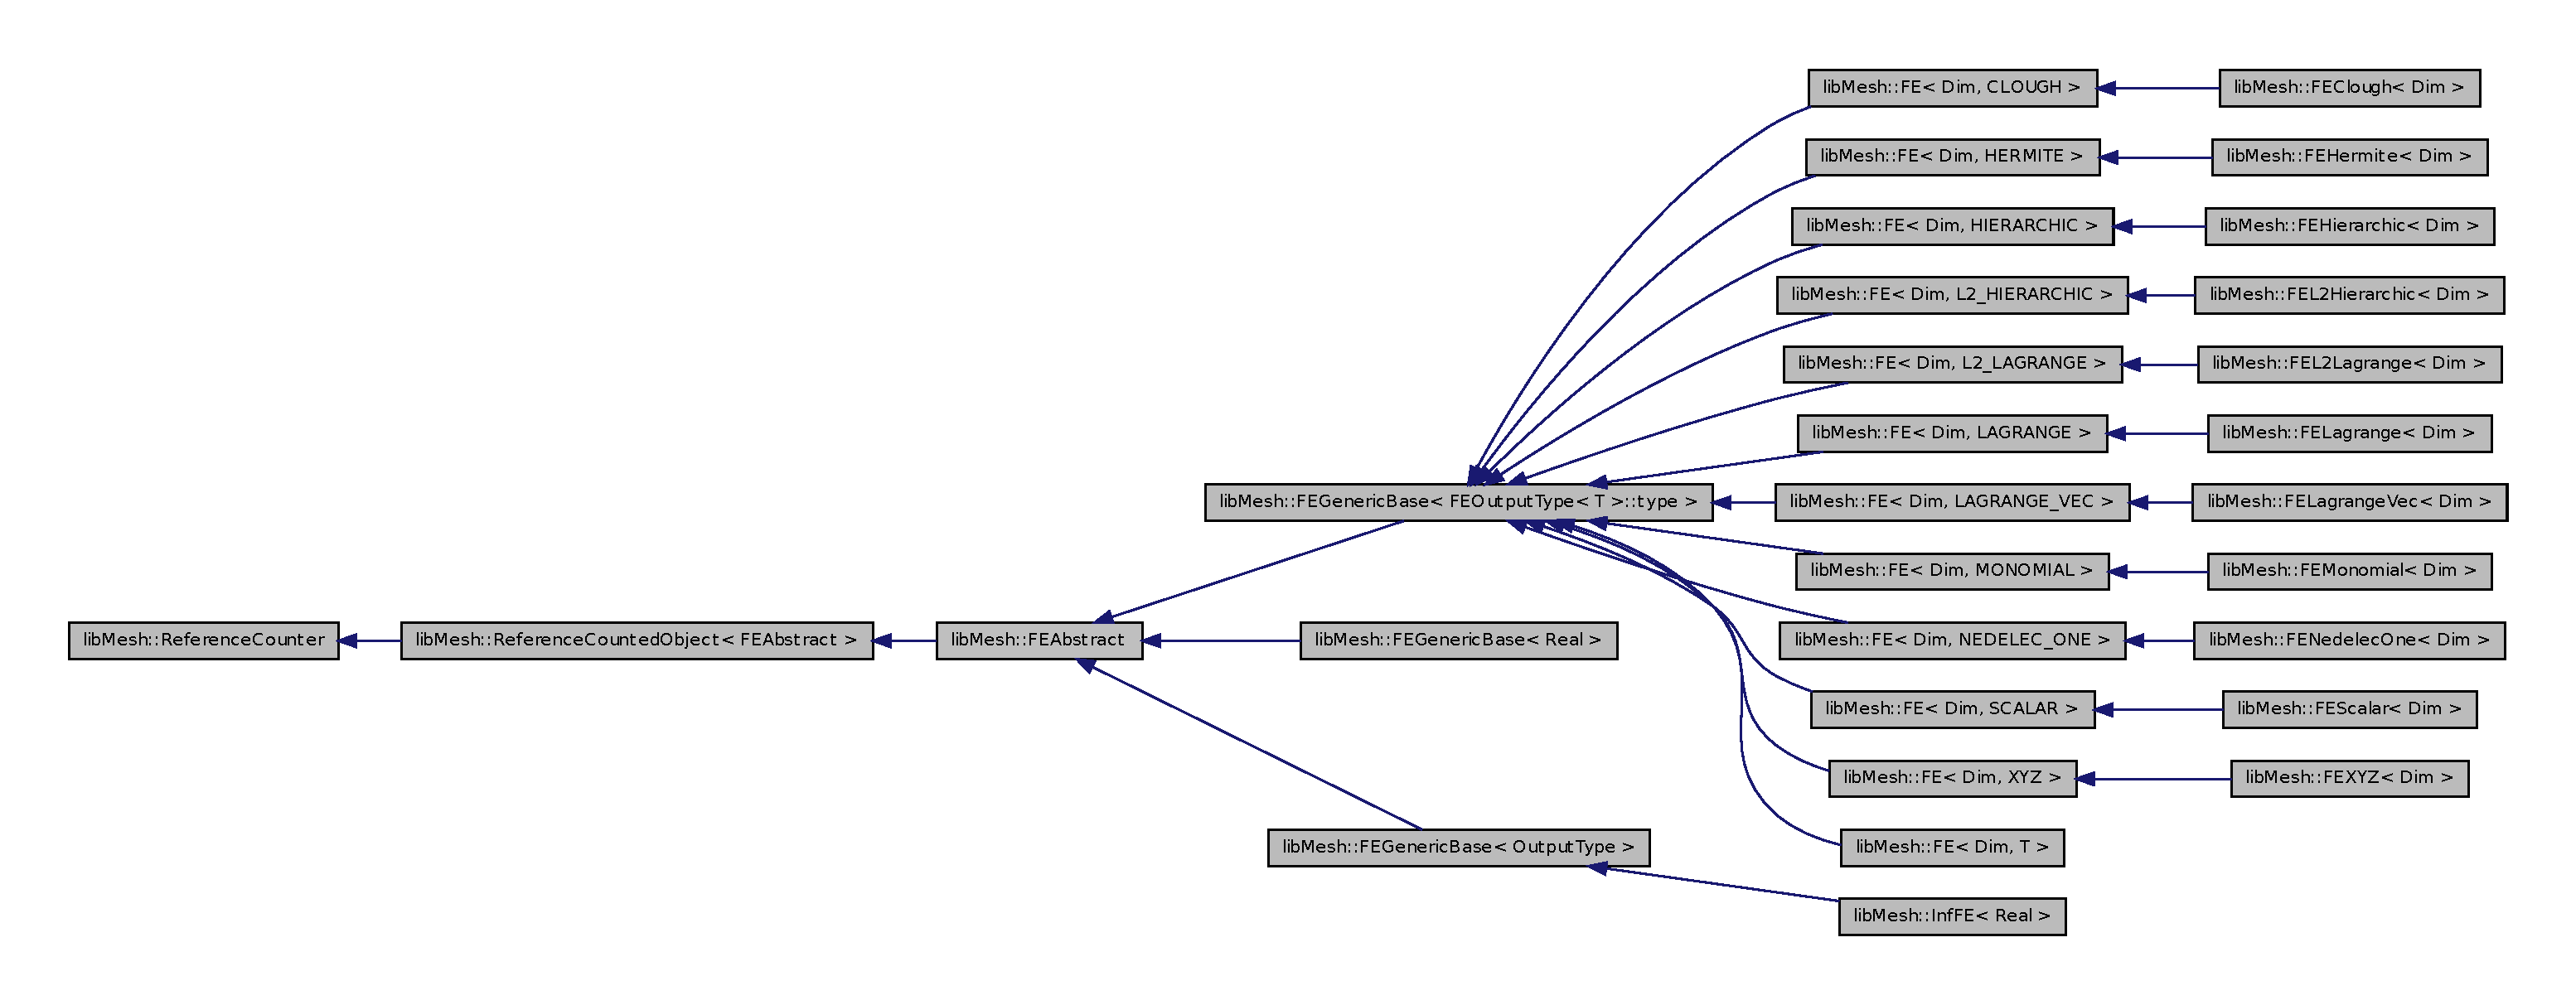
\includegraphics[width=0.9\textwidth,trim=7.4in 0 0 0,clip]{libmesh_docs/classlibMesh_1_1FEAbstract__inherit__graph}
  \end{center}
}      



%%%%%%%%%%%%%%%%%%%%%%%%%%%%%%%%%%%%%%%%%%%%%%%%%
\frame
{
  \frametitle{Algorithms: Domain Partitioning}
  \begin{center}
    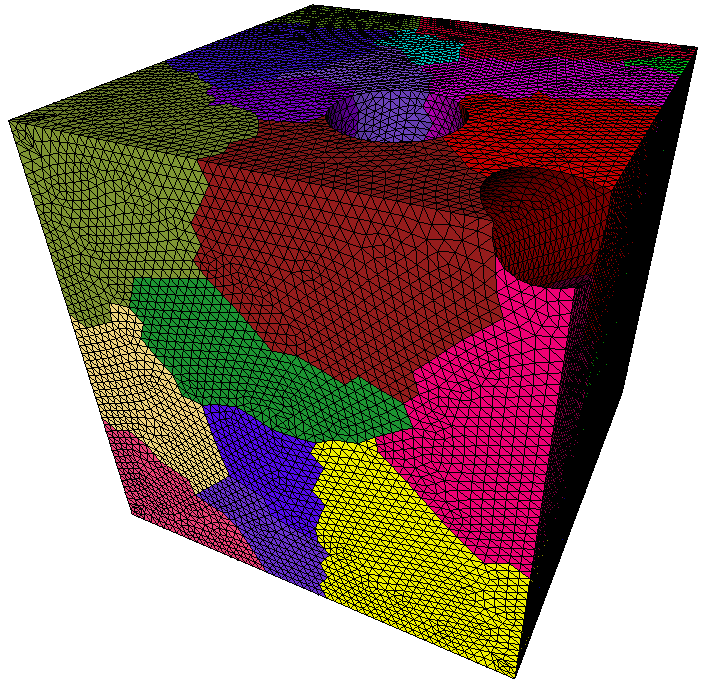
\includegraphics[width=.45\textwidth]{part_trans}
    %\\
    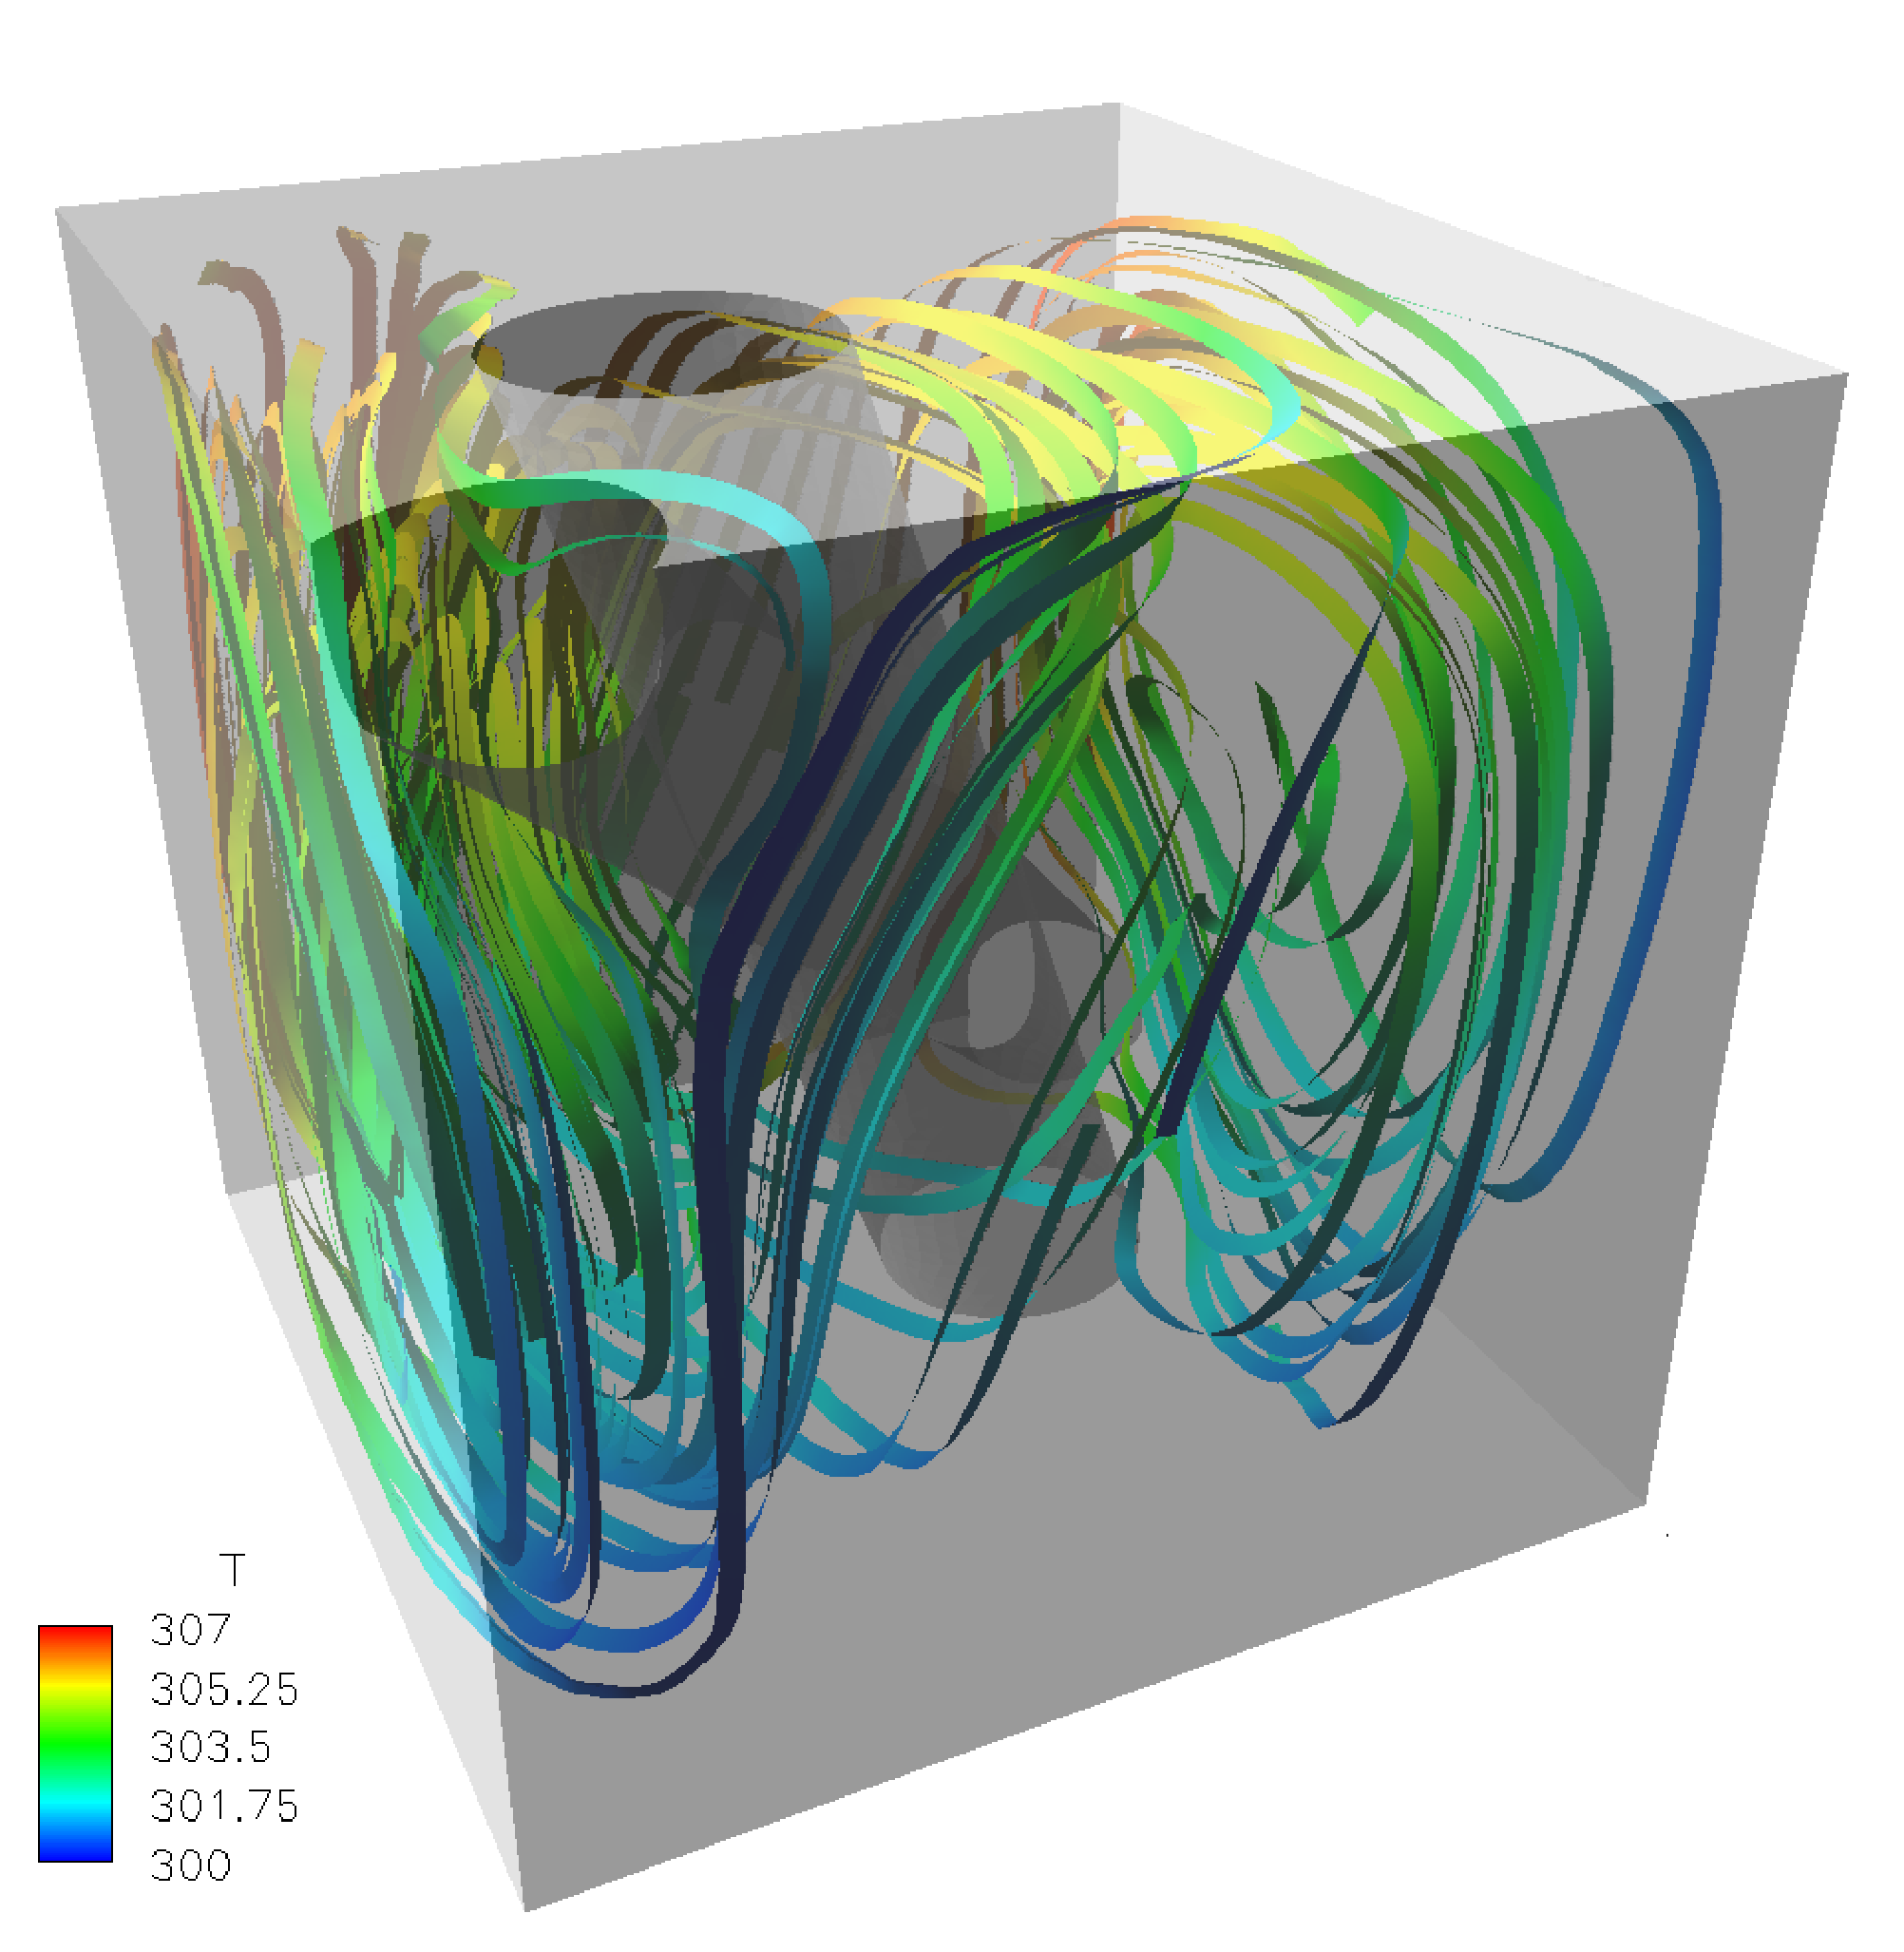
\includegraphics[width=.45\textwidth]{streamtraces}
  \end{center}  
}



%%%%%%%%%%%%%%%%%%%%%%%%%%%%%%%%%%%%%%%%%%%%%%%%%
\frame
{
  \frametitle{Algorithms: Domain Partitioning}
  \begin{center}
    \includegraphics[width=\textwidth]{libmesh_docs/partitioner}
  \end{center}
}


%%%%%%%%%%%%%%%%%%%%%%%%%%%%%%%%%%%%%%%%%%%%%%%%%
\frame
{
  \frametitle{Algorithms: Error Estimation}
  \begin{center}
    \includegraphics[width=\textwidth]{libmesh_docs/error_estimation}
  \end{center}
}





% LocalWords:  nasablue

%\subsection*{Non-Trivial Applications}
\begin{frame}%[t]
%  \frametitle{Weighted Residual Connection}
  %\begin{block}{}
  \begin{itemize}%[<+->]
  \item{Common to each is the need
    to solve a linear system
    (or systems) of equations $\bv{K} \bv{U} = \bv{F}$.}

  \item{LibMesh provides several of the tools necessary to construct
    these systems, but it is not specifically written to solve any one
    problem.}

  \item{We now briefly show a few of the non-trivial applications which have been built on
    top of the library.}
    
%%   \item{In each case, the matrix $A$ is the ``Jacobian''
%%     operator, and the right-hand side vector $b$ is the
%%     weighted residual itself.}

    %% 	\item{This is true even in the case of linear $\R( u )$, since
    %% 	  in this case the linearized operator is
    %% 	  \begin{eqnarray}
    %% 	    \nonumber
    %% 	    \R'( u )w &:=& \lim_{\varepsilon\rightarrow 0}
    %% 	    \frac{\R(u+\varepsilon w) - \R(u)}{\varepsilon} \\
    %% 	    \nonumber
    %% 	    &=& \R(w)
    %% 	  \end{eqnarray}
    %% 	}
  \end{itemize}
%\end{block}
\end{frame}	  

%\subsection*{Natural Convection}
\begin{frame}[t]
  \begin{center}
    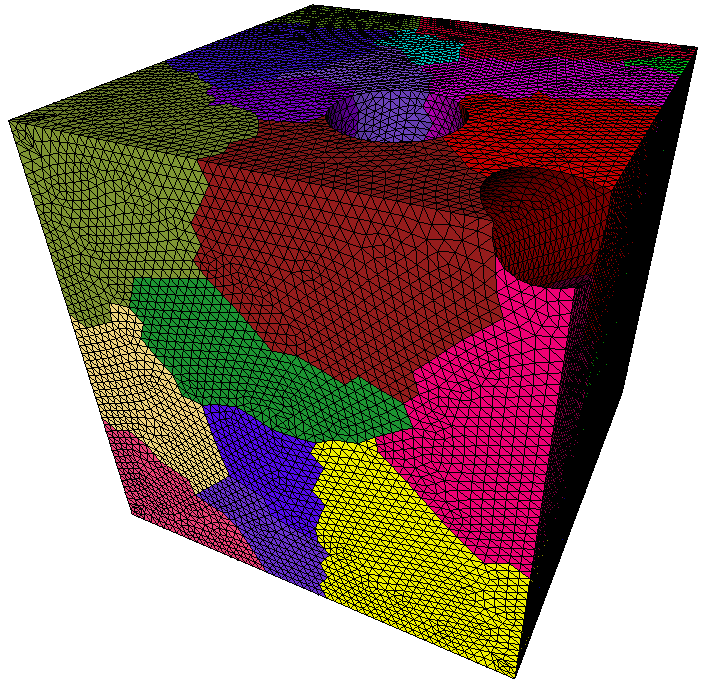
\includegraphics[width=.45\textwidth]{part_trans}
    %\\
    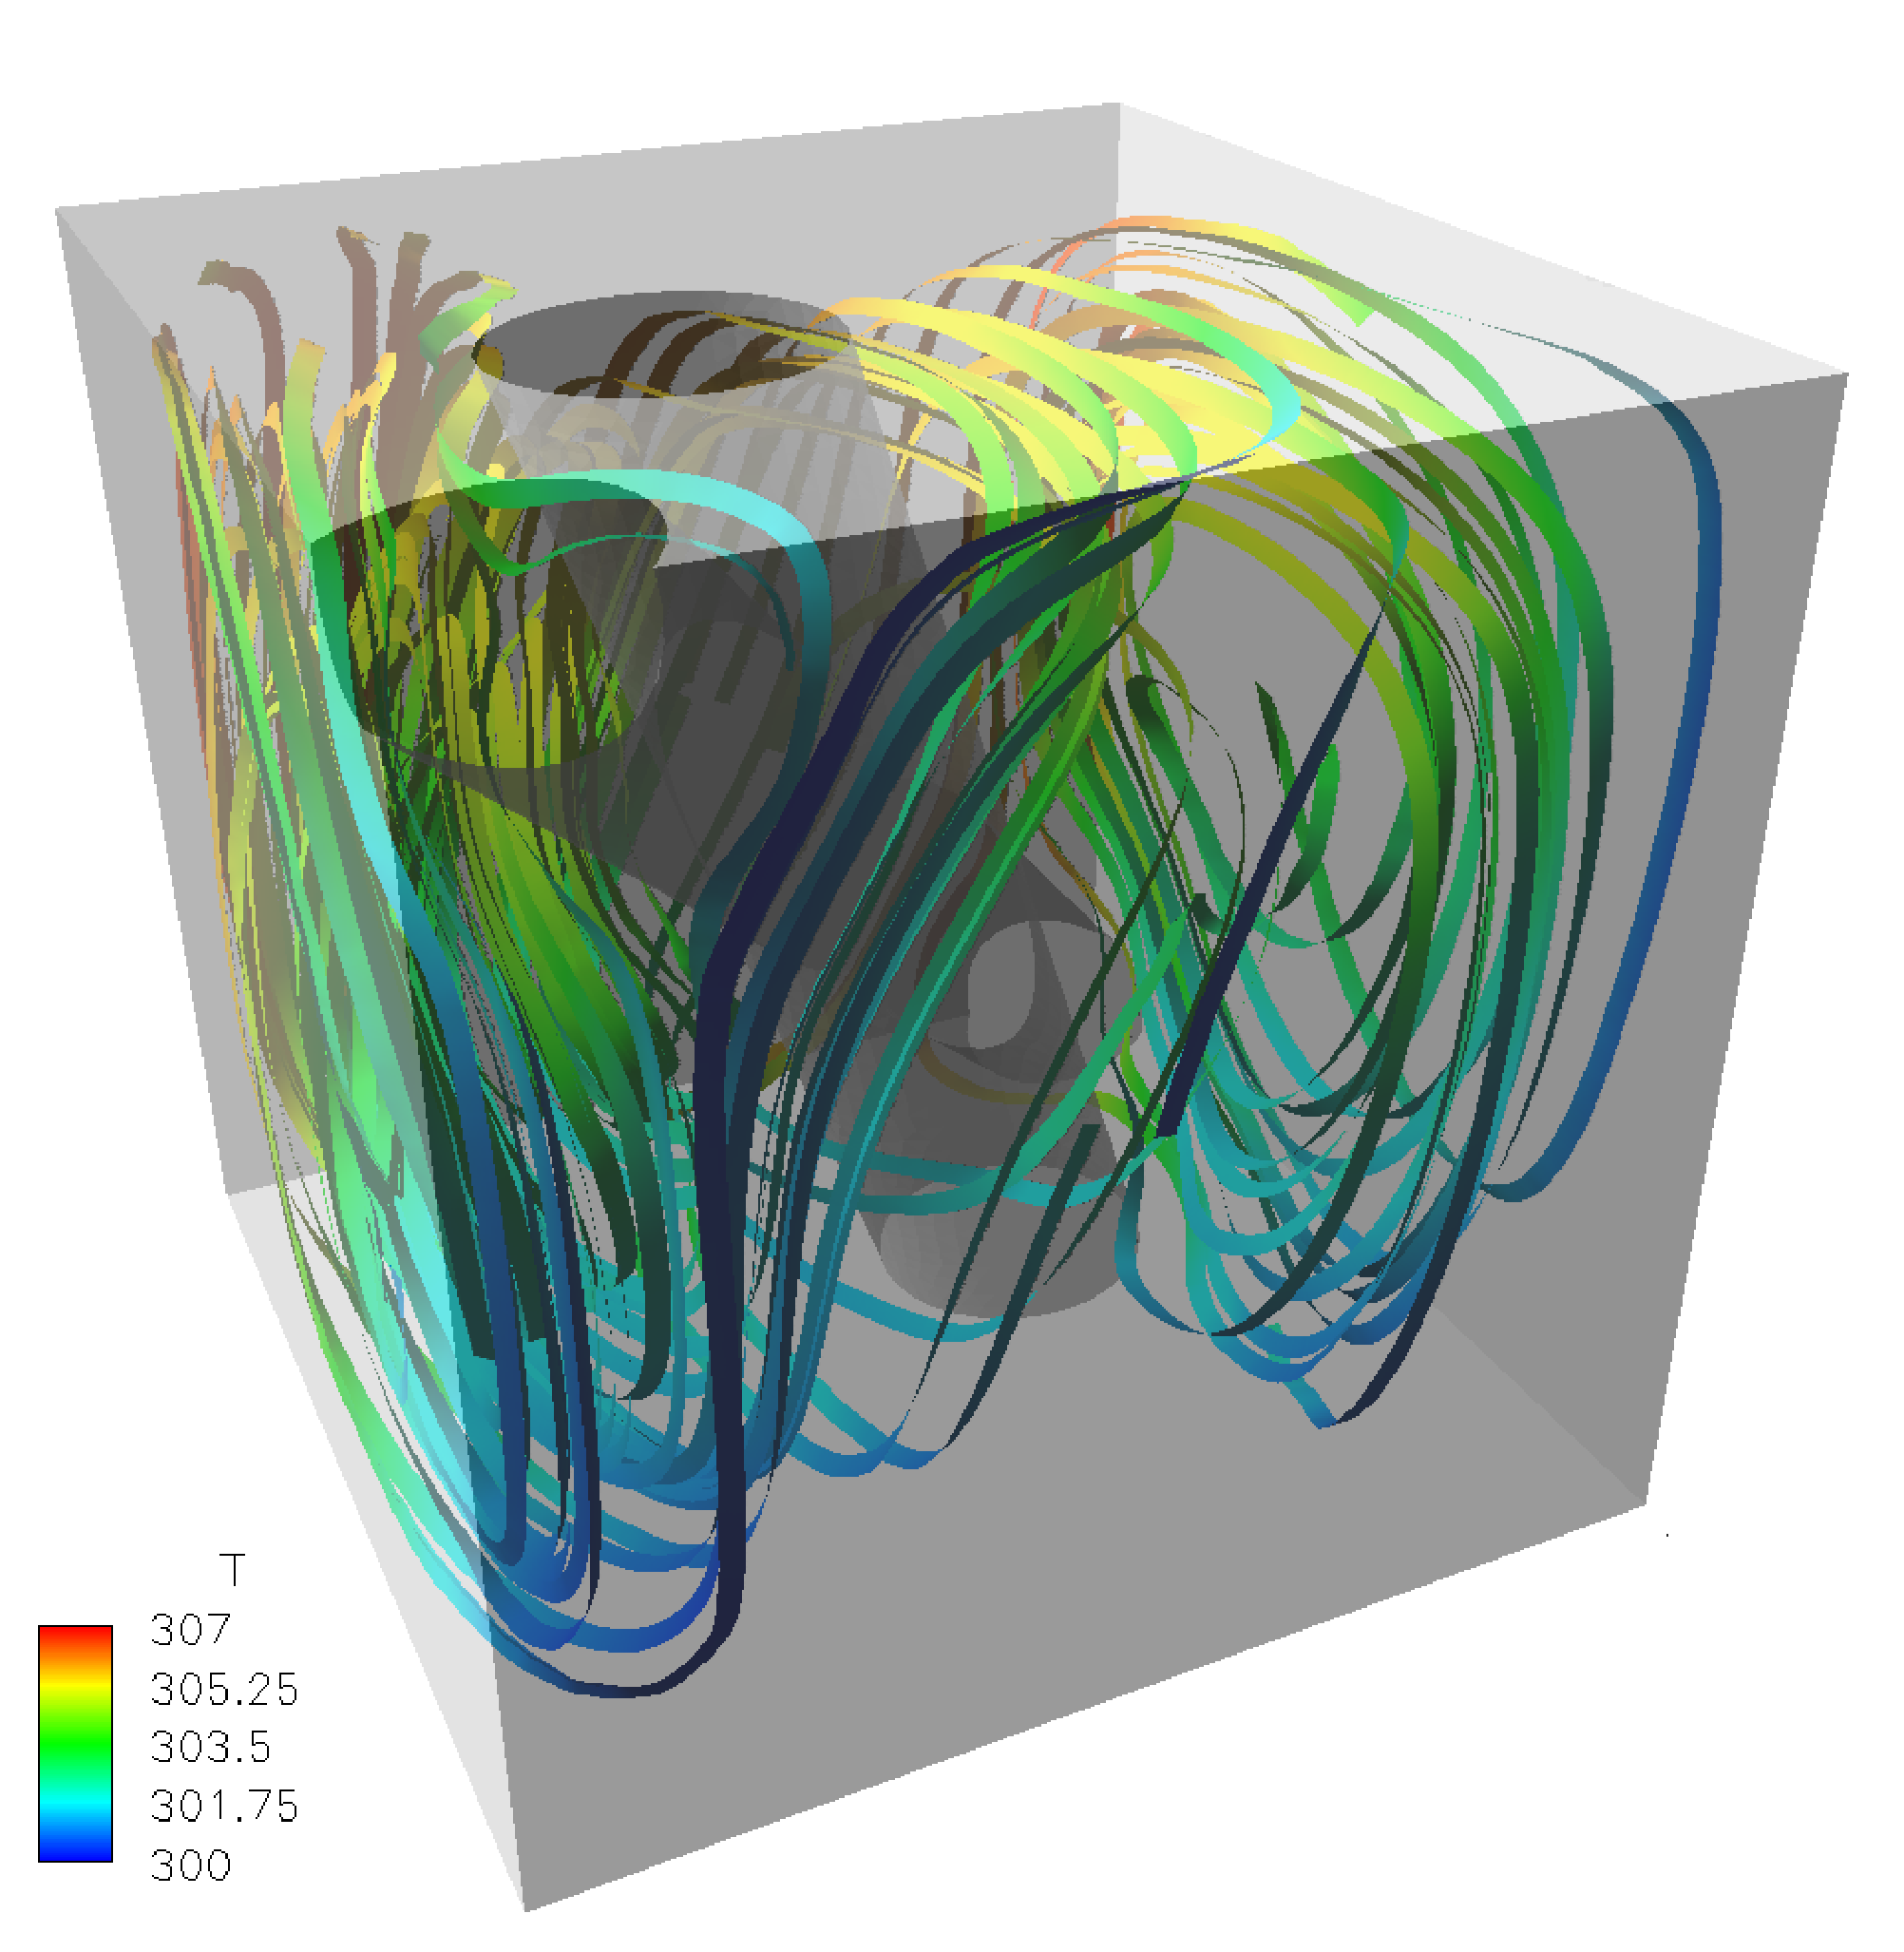
\includegraphics[width=.45\textwidth]{streamtraces}
  \end{center}
  \begin{block}{}
    \begin{itemize}
    \item{
      Tetrahedral mesh of ``pipe'' geometry.
      Stream ribbons colored by temperature.
      }
      \end{itemize}
  \end{block}
\end{frame}

%\begin{frame}[t]
  \frametitle{Surface-Tension-Driven Flow}
  \begin{center}
    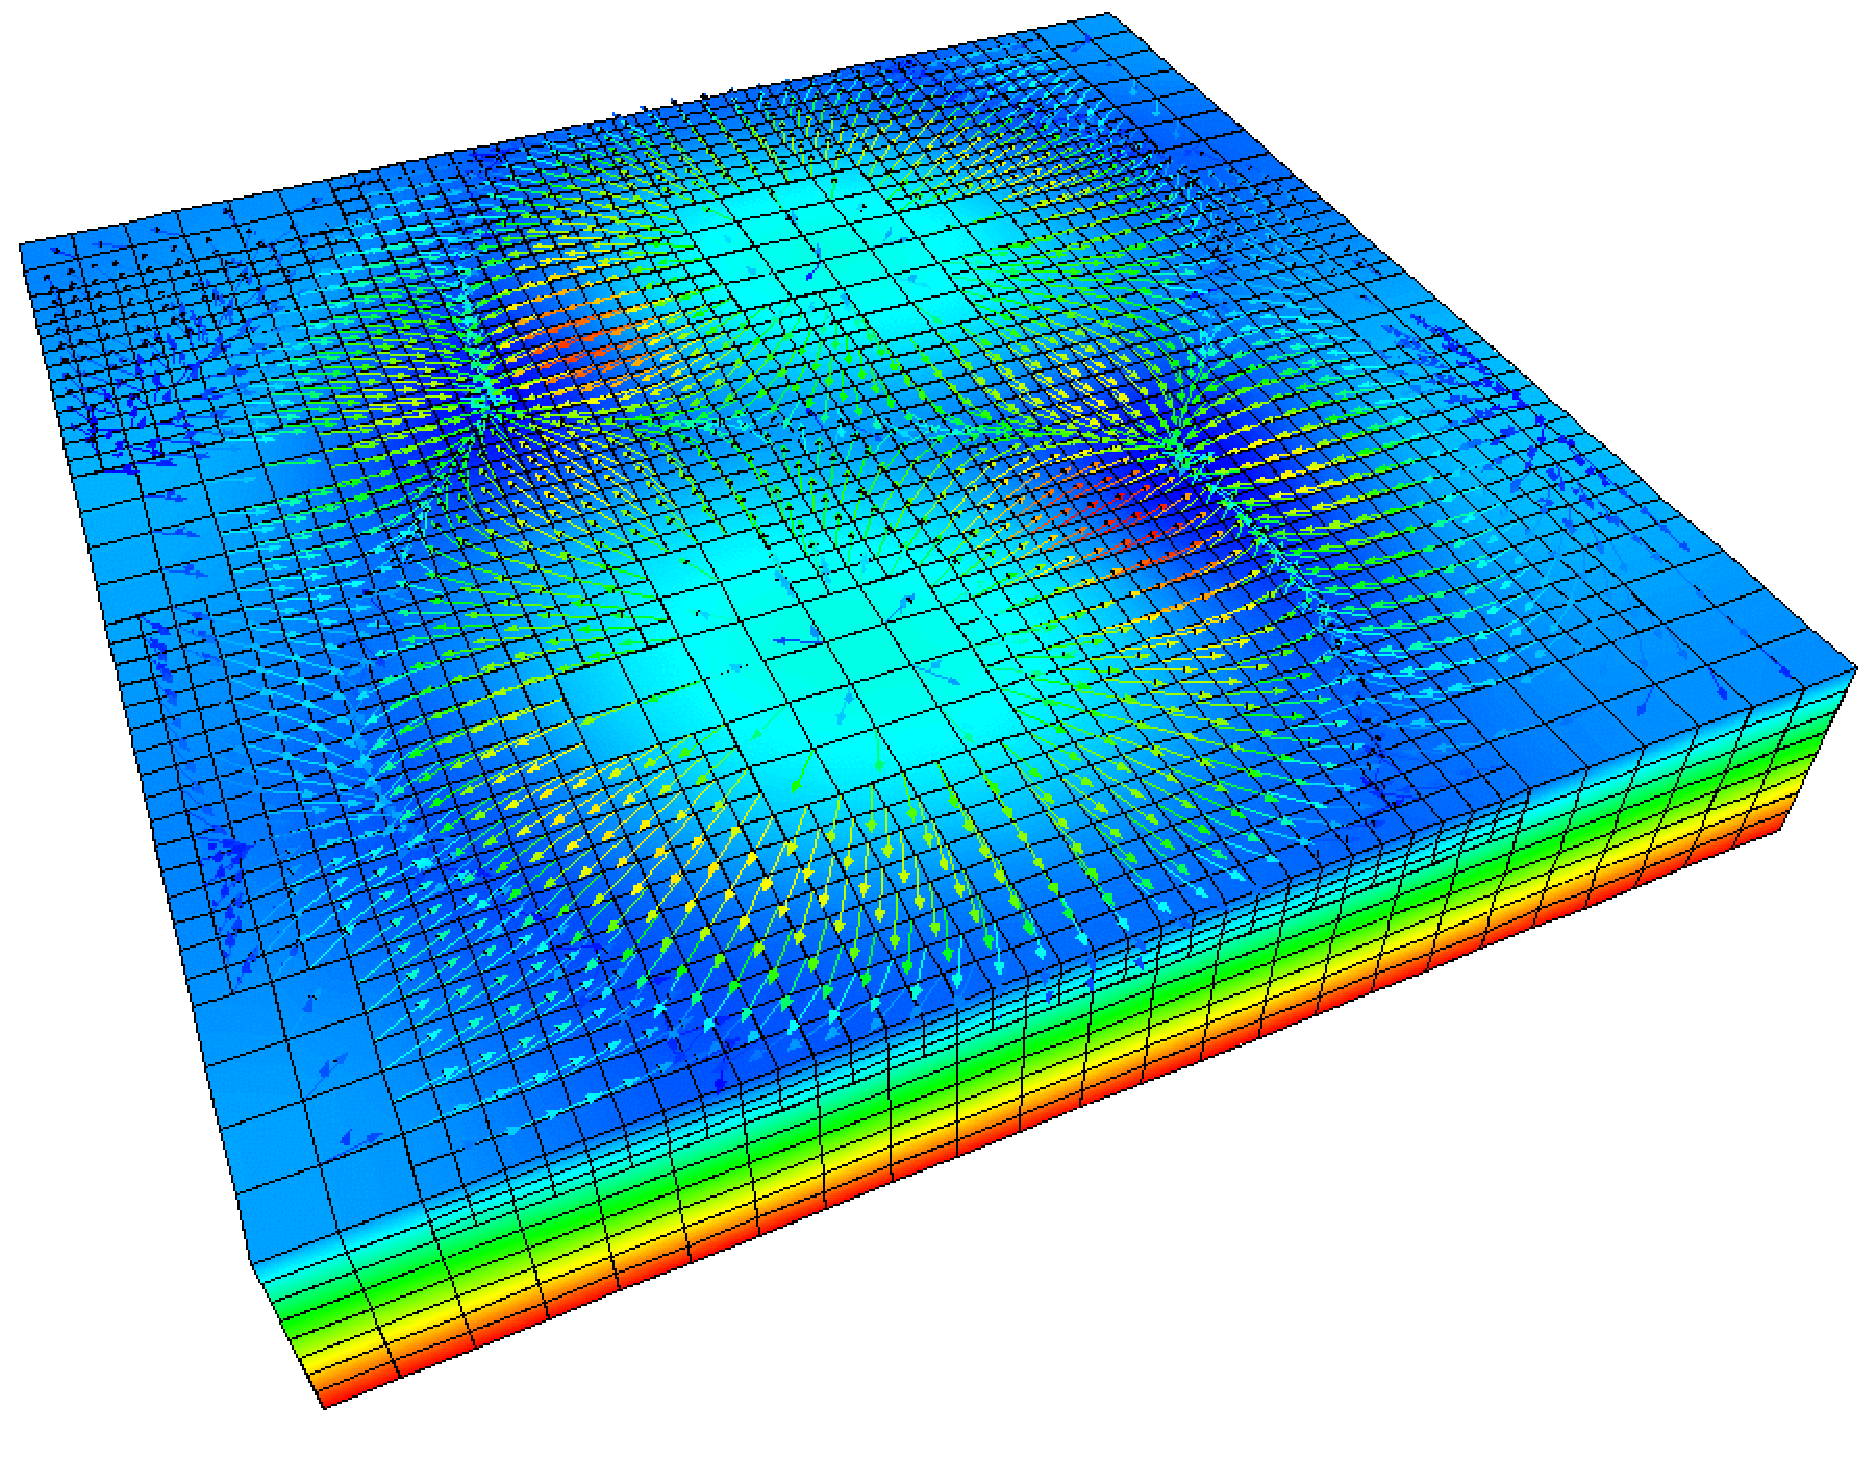
\includegraphics[width=.6\textwidth]{figs/rbm_adapt_soln}    
  \end{center}

  \begin{block}{}
    \begin{itemize}
    \item{Adaptive grid solution shown
      with temperature contours and velocity vectors.
      }
      \end{itemize}
  \end{block}
\end{frame}

%\begin{frame}[t]
  \frametitle{Double-Diffusive Convection}
  \begin{center}
    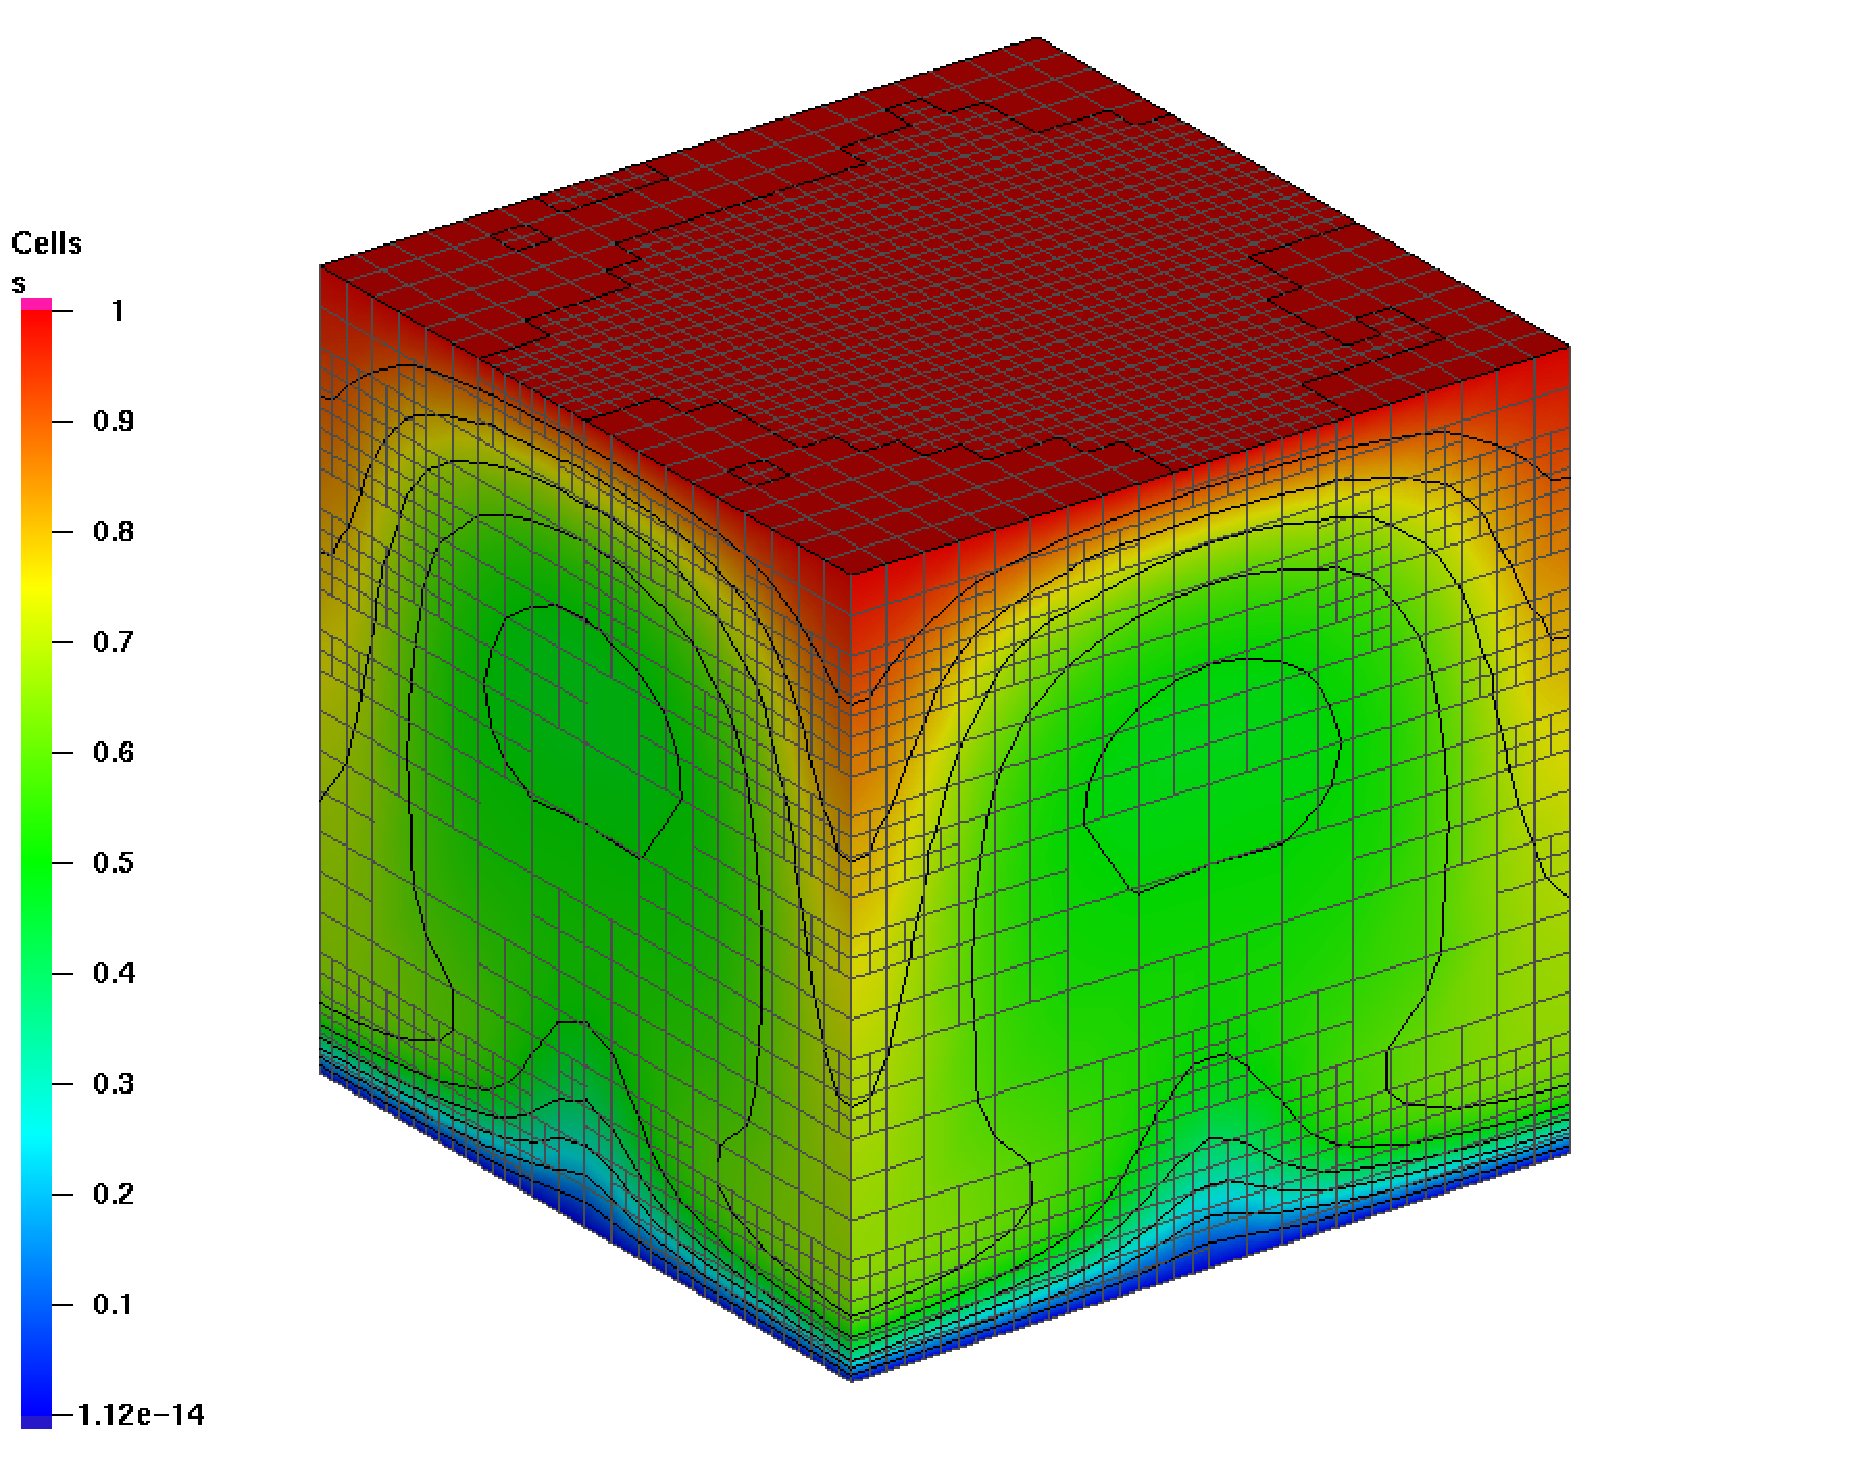
\includegraphics[width=.6\textwidth]{figs/dd}    
  \end{center}

  \begin{block}{}
    \begin{itemize}
    \item{Solute contours: a plume of
      warm, low-salinity fluid is convected upward through a porous medium.
      }
      \end{itemize}
  \end{block}
\end{frame}



%\subsection*{Tumor Angiogenesis}
\begin{frame}[t]
  \begin{center}
    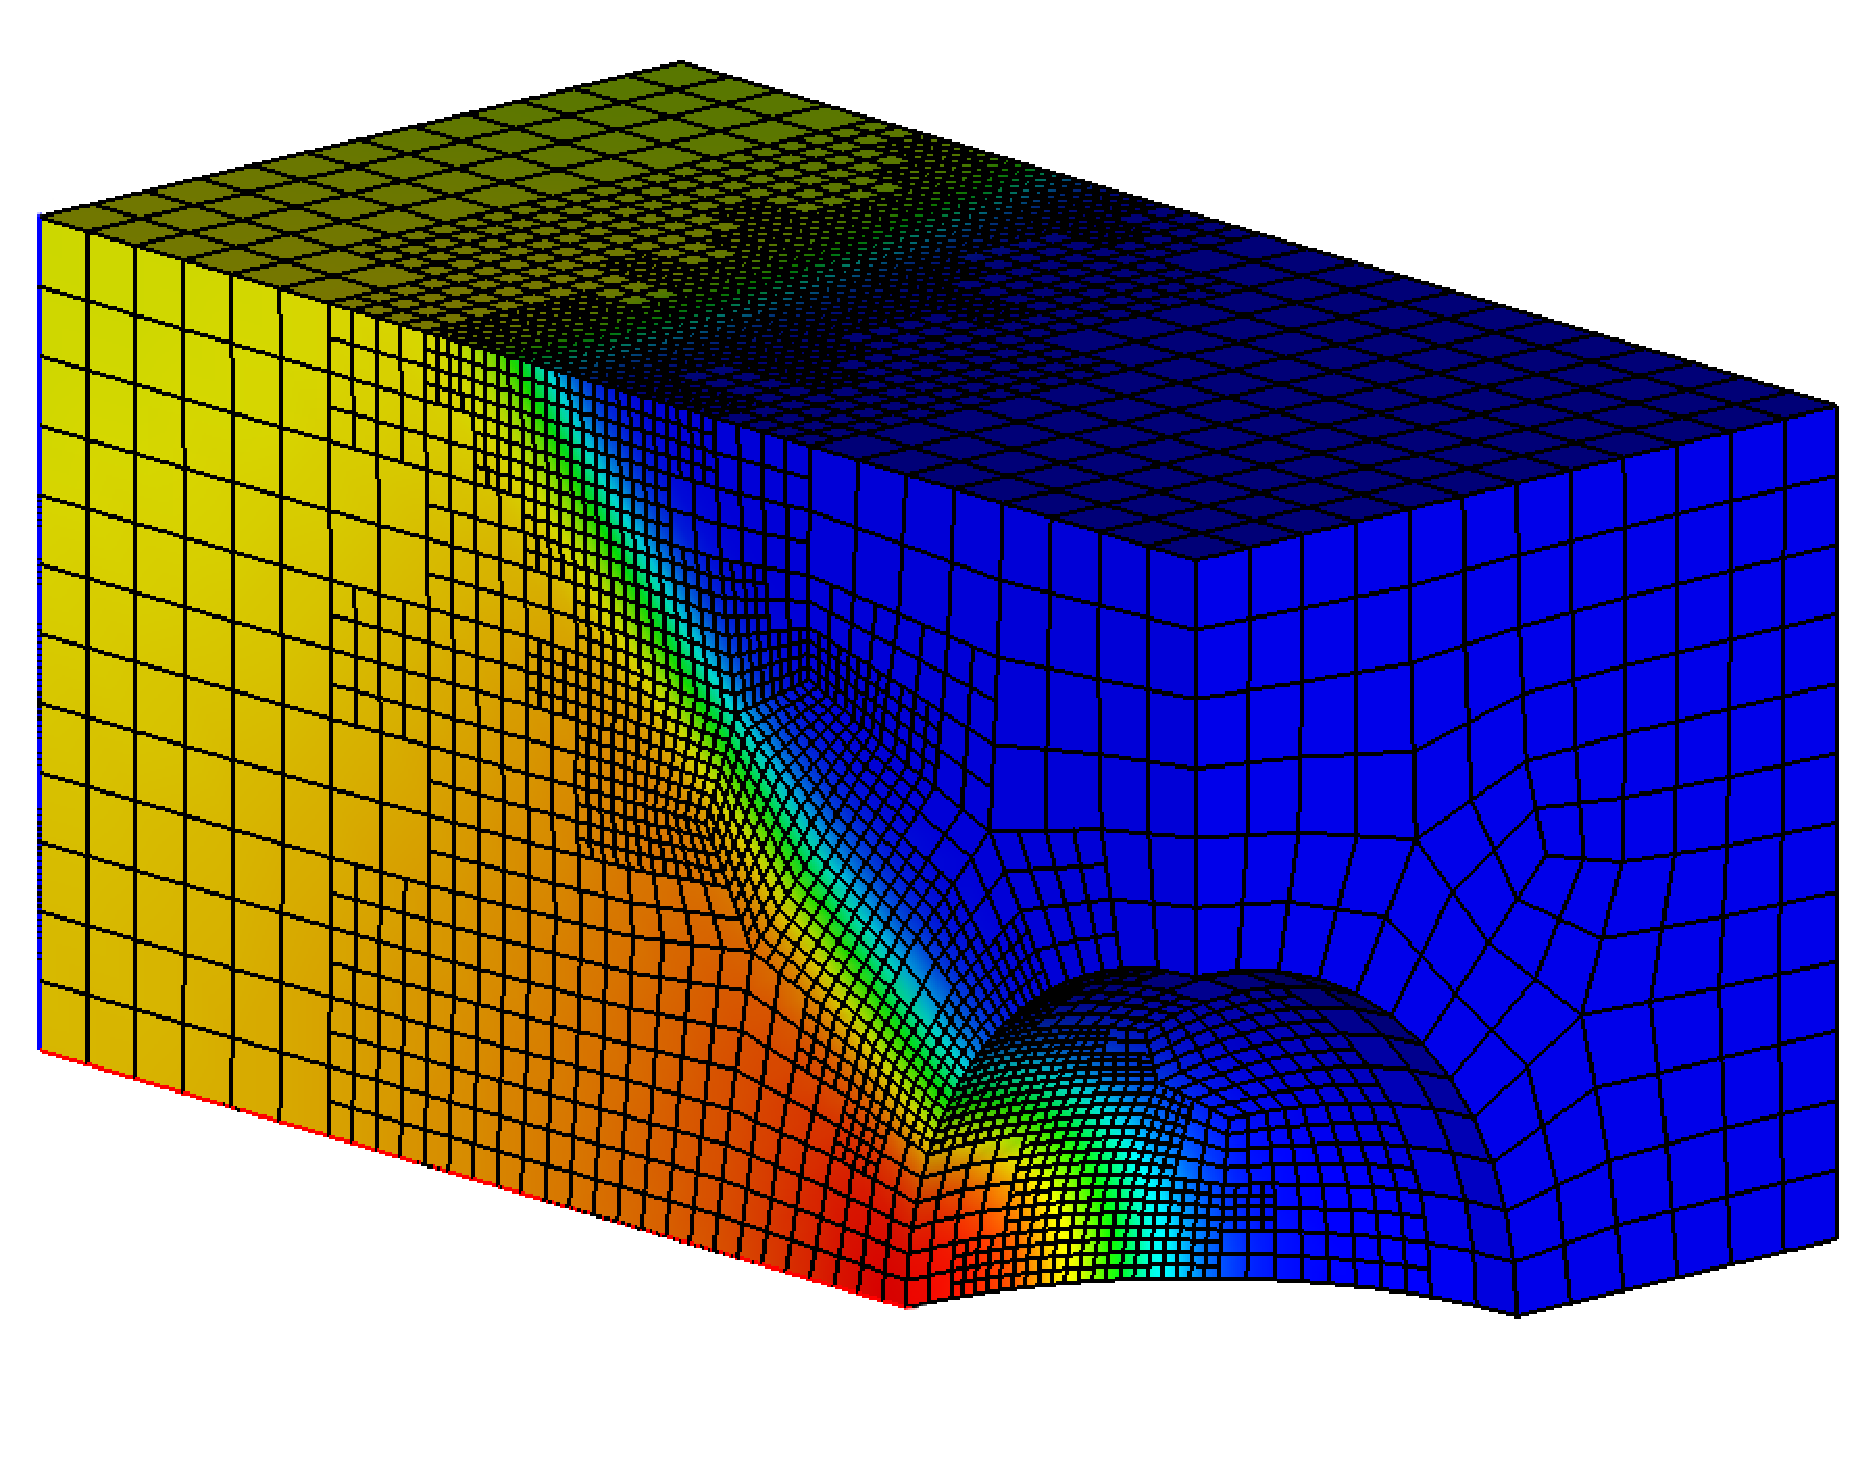
\includegraphics[width=.6\textwidth]{tumor_model}    
  \end{center}

  \begin{block}{}
    \begin{itemize}
    \item{%Tumor angiogenesis model simulation.
      The tumor secretes
      a chemical which stimulates blood vessel formation.
      }
      \end{itemize}
  \end{block}
\end{frame}



%%%%%%%%%%%%%%%%%%%%%%%%%%%%%%%%%%%%%%%%%%%%%%%%%%%%%%%%%%%%%%%%%%%%%%
\royslide{Free Energy Formulation}{

Cahn-Hilliard systems model phase separation and interface
evolution

\begin{eqnarray*}
f(c, \nabla c) & \equiv & f_0(c) + f_\gamma(\nabla c) \\
f_\gamma(\nabla c) & \equiv & \frac{\epsilon_c^2}{2} \nabla c \cdot \nabla c \\
%f_{0m}(c) & \equiv & \frac{1}{4} \left( c^2 - 1 \right)^2 \\
f_0(c) & \equiv & N k T \left( c \ln{(c)} + 
(1-c) \ln{(1-c)} \right) + 
N \omega c (1-c)
\end{eqnarray*}

\begin{eqnarray*}
\dt{c} & = & \nabla \cdot M_c \nabla
  \left( f_0'(c) - \epsilon_c^2 \Laplacian c \right)
\end{eqnarray*}
}


%\subsection*{Compressible Flow}

\frame
{
  \frametitle{Compressible Shocked Flow}
  \begin{itemize}[<+->]
    \item Original compressible flow code written by Ben Kirk utilizing libMesh.
      \begin{itemize}[<+->]
      \item Solves both Compressible Navier Stokes and Inviscid Euler.
      \item Includes both SUPG and a shock capturing scheme.
      \end{itemize}
    \item Original redistribution code written by Larisa Branets.
      \begin{itemize}[<+->]
      \item Simultaneous optimization of element shape and size.
      \item Directable via user supplied error estimate.
      \end{itemize}
    \item Integration work done by Derek Gaston.
      \begin{itemize}[<+->]
      \item Combination of redistribution, $h$ refinement.
      \item Applicable to other problem classes.
      \end{itemize}
  \end{itemize}
}

\frame
{
  \frametitle{Problem Specification}
  \begin{itemize}[<+->]
    \item The problem studied is that of an oblique shock generated by a $10^o$ wedge angle. 
      \begin{itemize}[<+->]
      \item This problem has an exact solution for density which is a step function.
      \item Utilizing libmesh's exact solution capability the exact
$L_2$ error can be solved for.
      \item The exact solution is shown below:
        \begin{figure}
          \begin{center}
            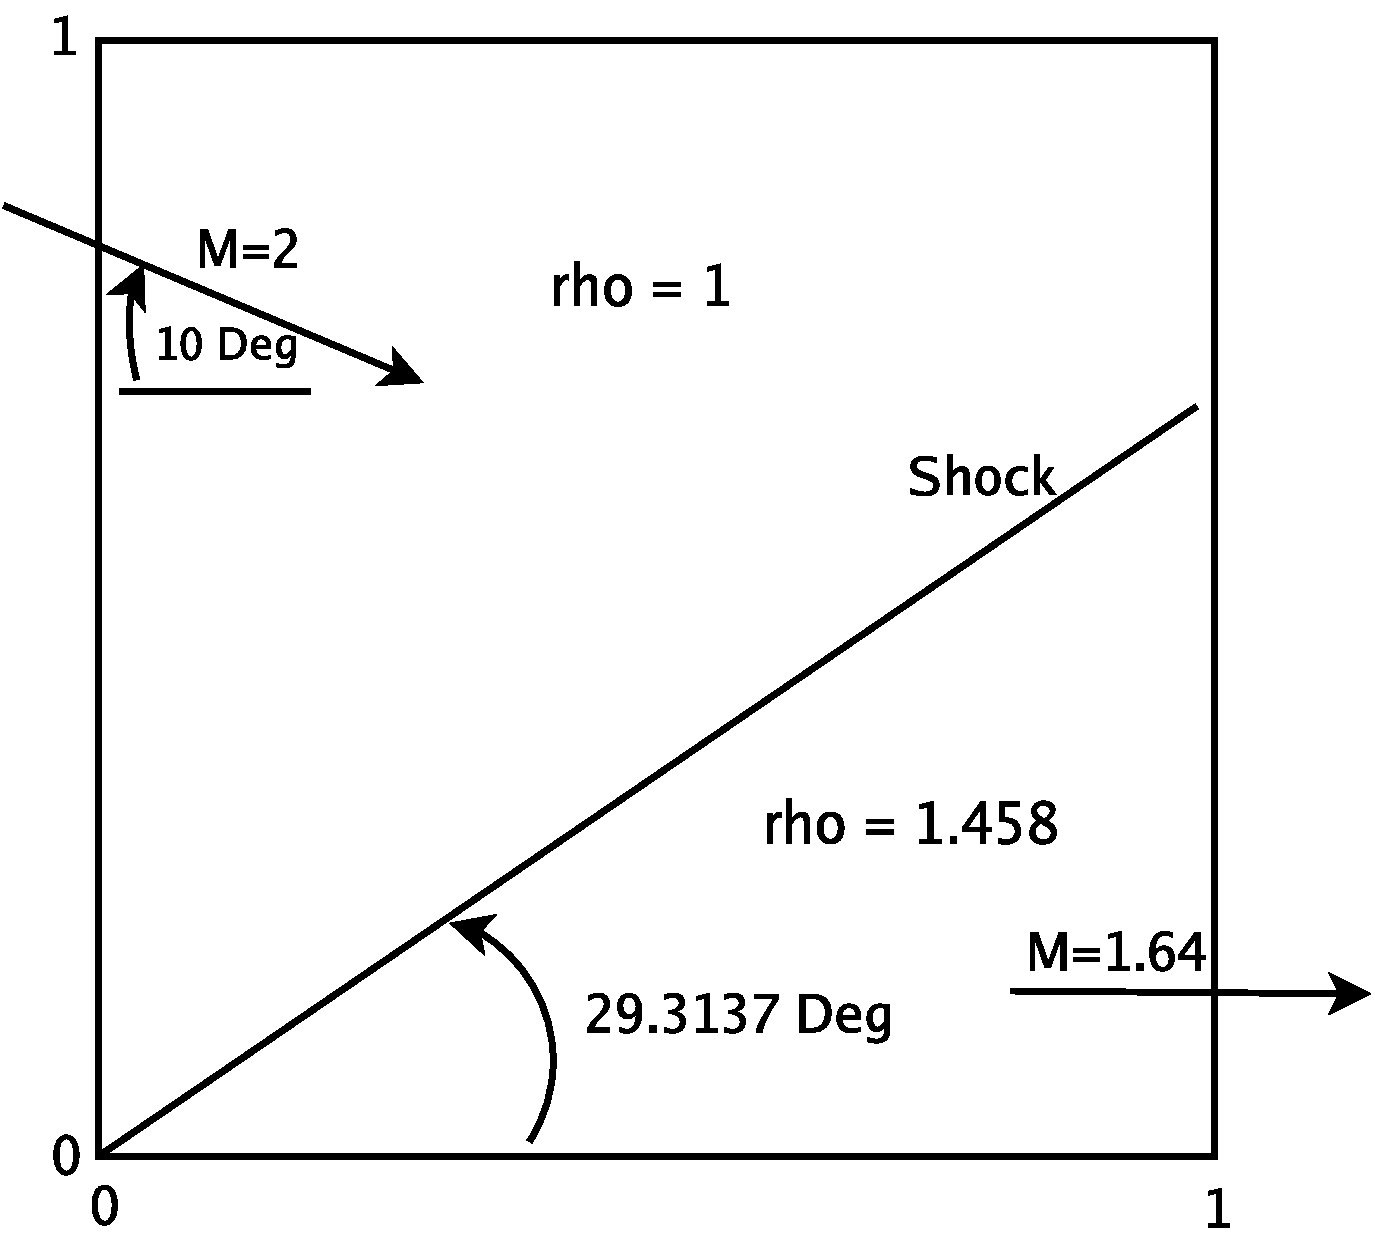
\includegraphics[viewport=20 10 660 600,clip=true,width=.4\textwidth]{shock.pdf}
          \end{center}
        \end{figure}
    \end{itemize}
  \end{itemize}
}

\frame
{
  \frametitle{Uniformly Refined Solutions}
  \begin{itemize}[<+->]
  \item For comparison purposes, here is a mesh and a solution after 1 uniform refinement with 10890 DOFs.
    \begin{figure}[!htb]
      \begin{center}
        \subfigure[Mesh after 1 uniform refinement.]{\label{fig:fob_uniform_2_mesh}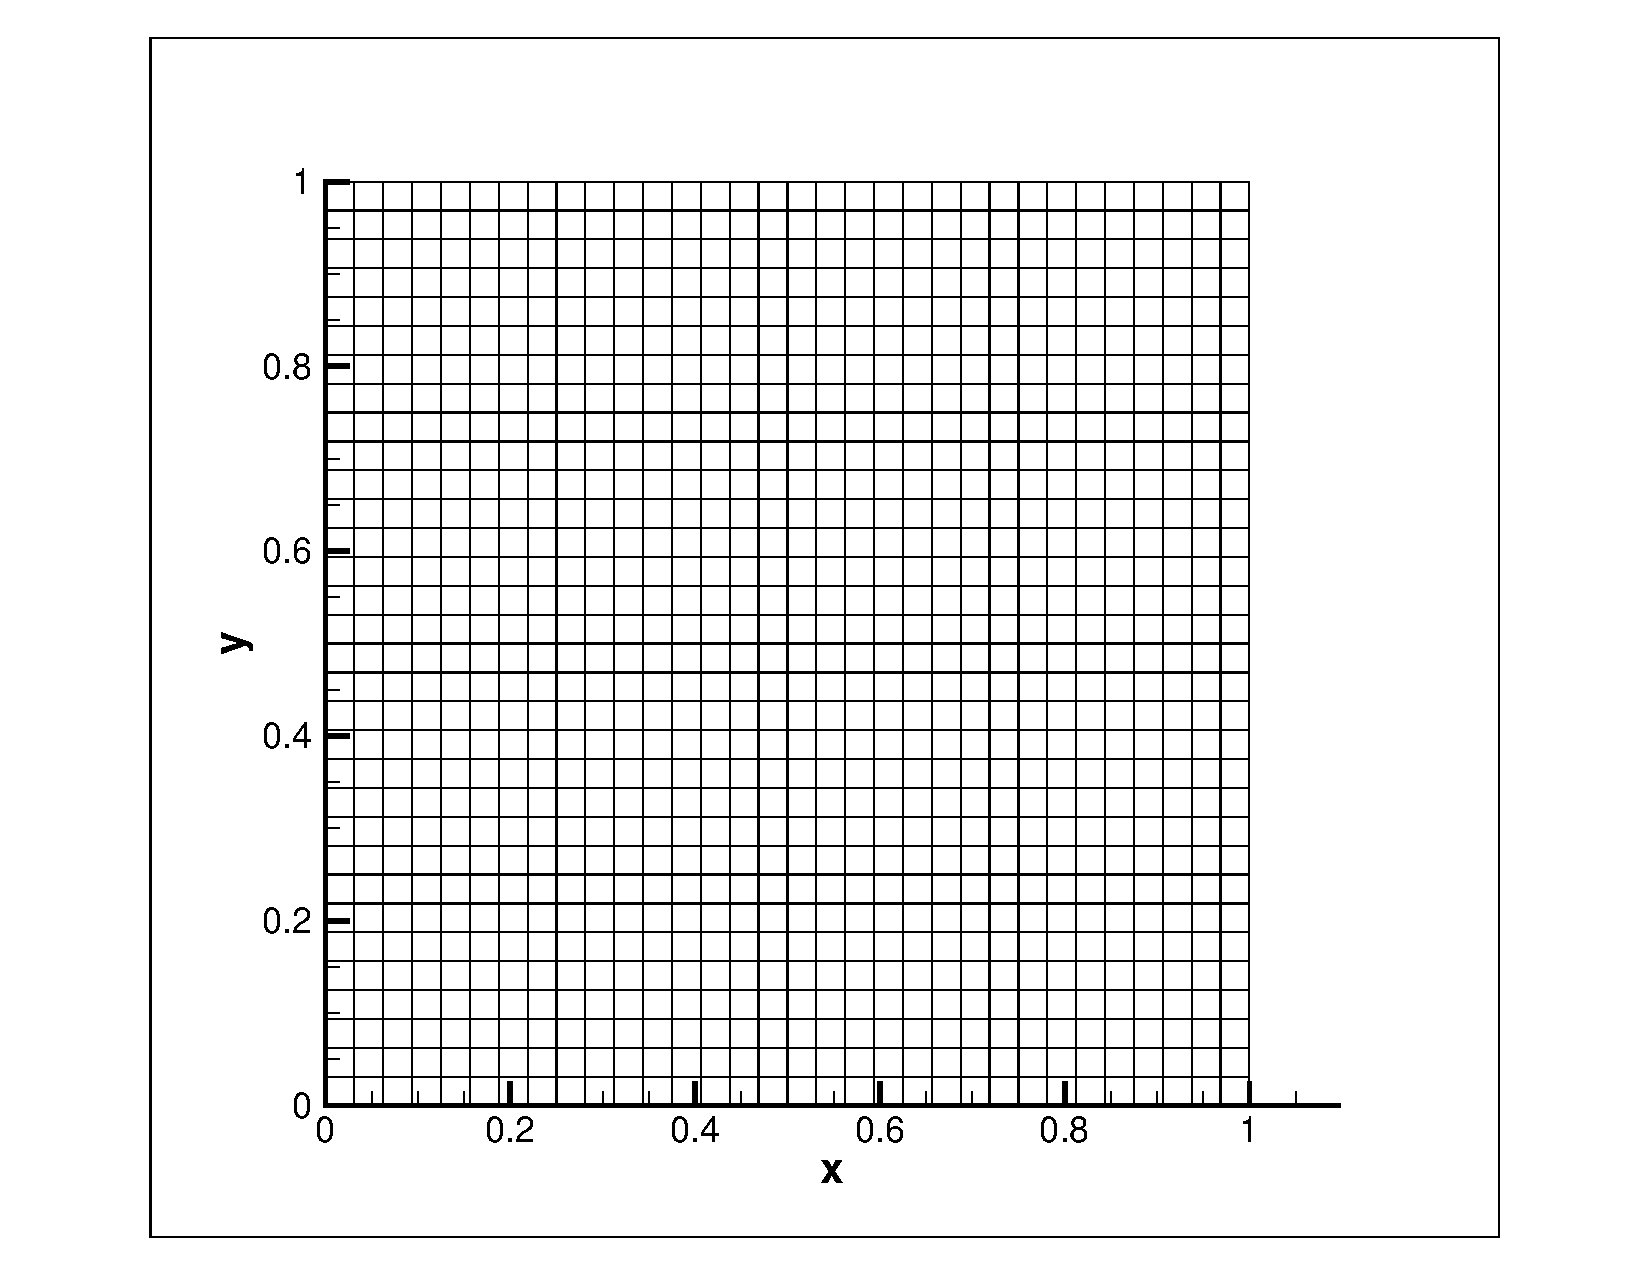
\includegraphics[viewport=110 30 600 550,clip=true,width=.42\textwidth]{fob_uniform_2_mesh.pdf}}
        \subfigure[Solution after 1 uniform refinement.]{\label{fig:fob_uniform_2_sol}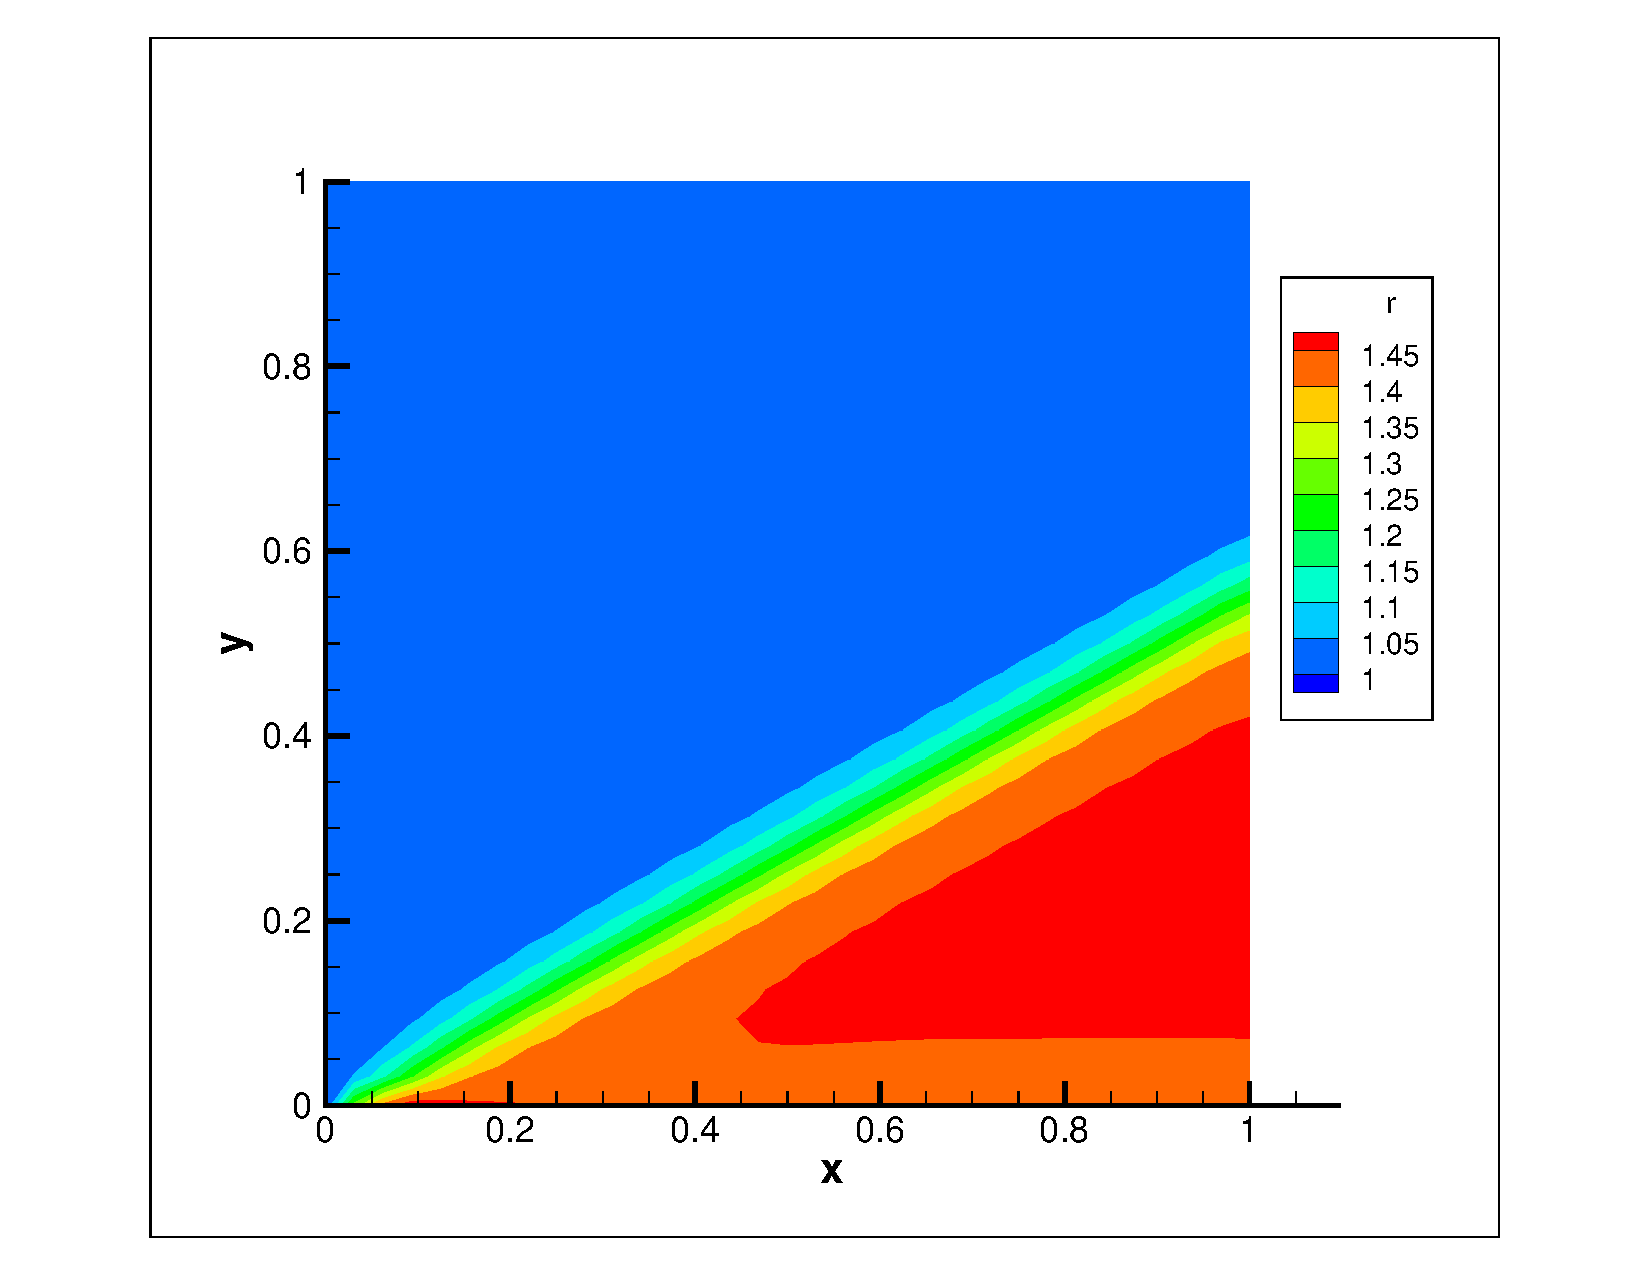
\includegraphics[viewport=110 30 600 520,clip=true,width=.42\textwidth]{fob_uniform_2_sol.pdf}}
      \end{center}
    \end{figure}
  \end{itemize}
}

\frame
{
  \frametitle{H-Adapted Solutions}
  \begin{itemize}[<+->]
    \item A flux jump indicator was employed as the error indcator along with a statistical flagging scheme.
    \item Here is a mesh and solution after 2 adaptive refinements containing 10800 DOFs:
      \begin{figure}[!htb]
        \begin{center}
          \subfigure[Mesh, 2 refinements]{\label{fig:fob_adapt_3_mesh}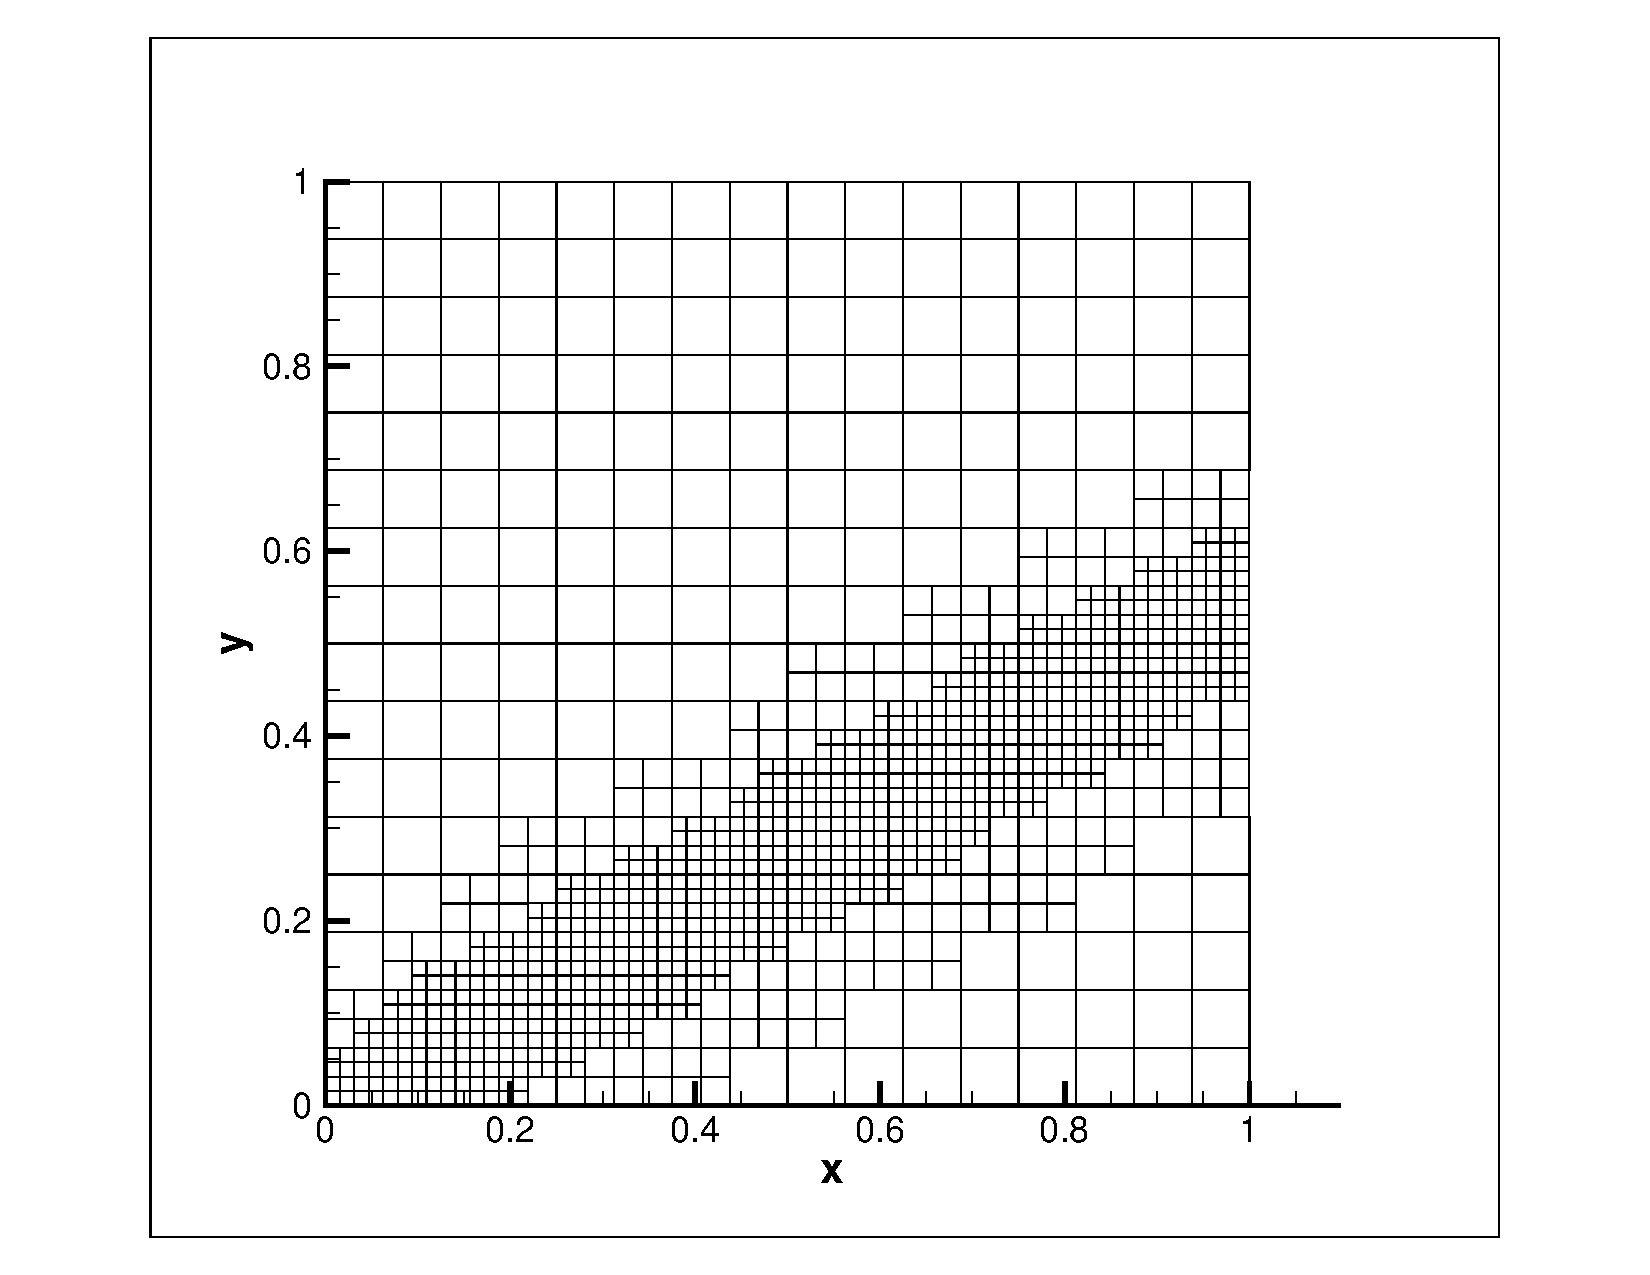
\includegraphics[viewport=110 30 600 550,clip=true,width=.42\textwidth]{fob_adapt_3_mesh.pdf}}
          \subfigure[Solution]{\label{fig:fob_adapt_3_sol}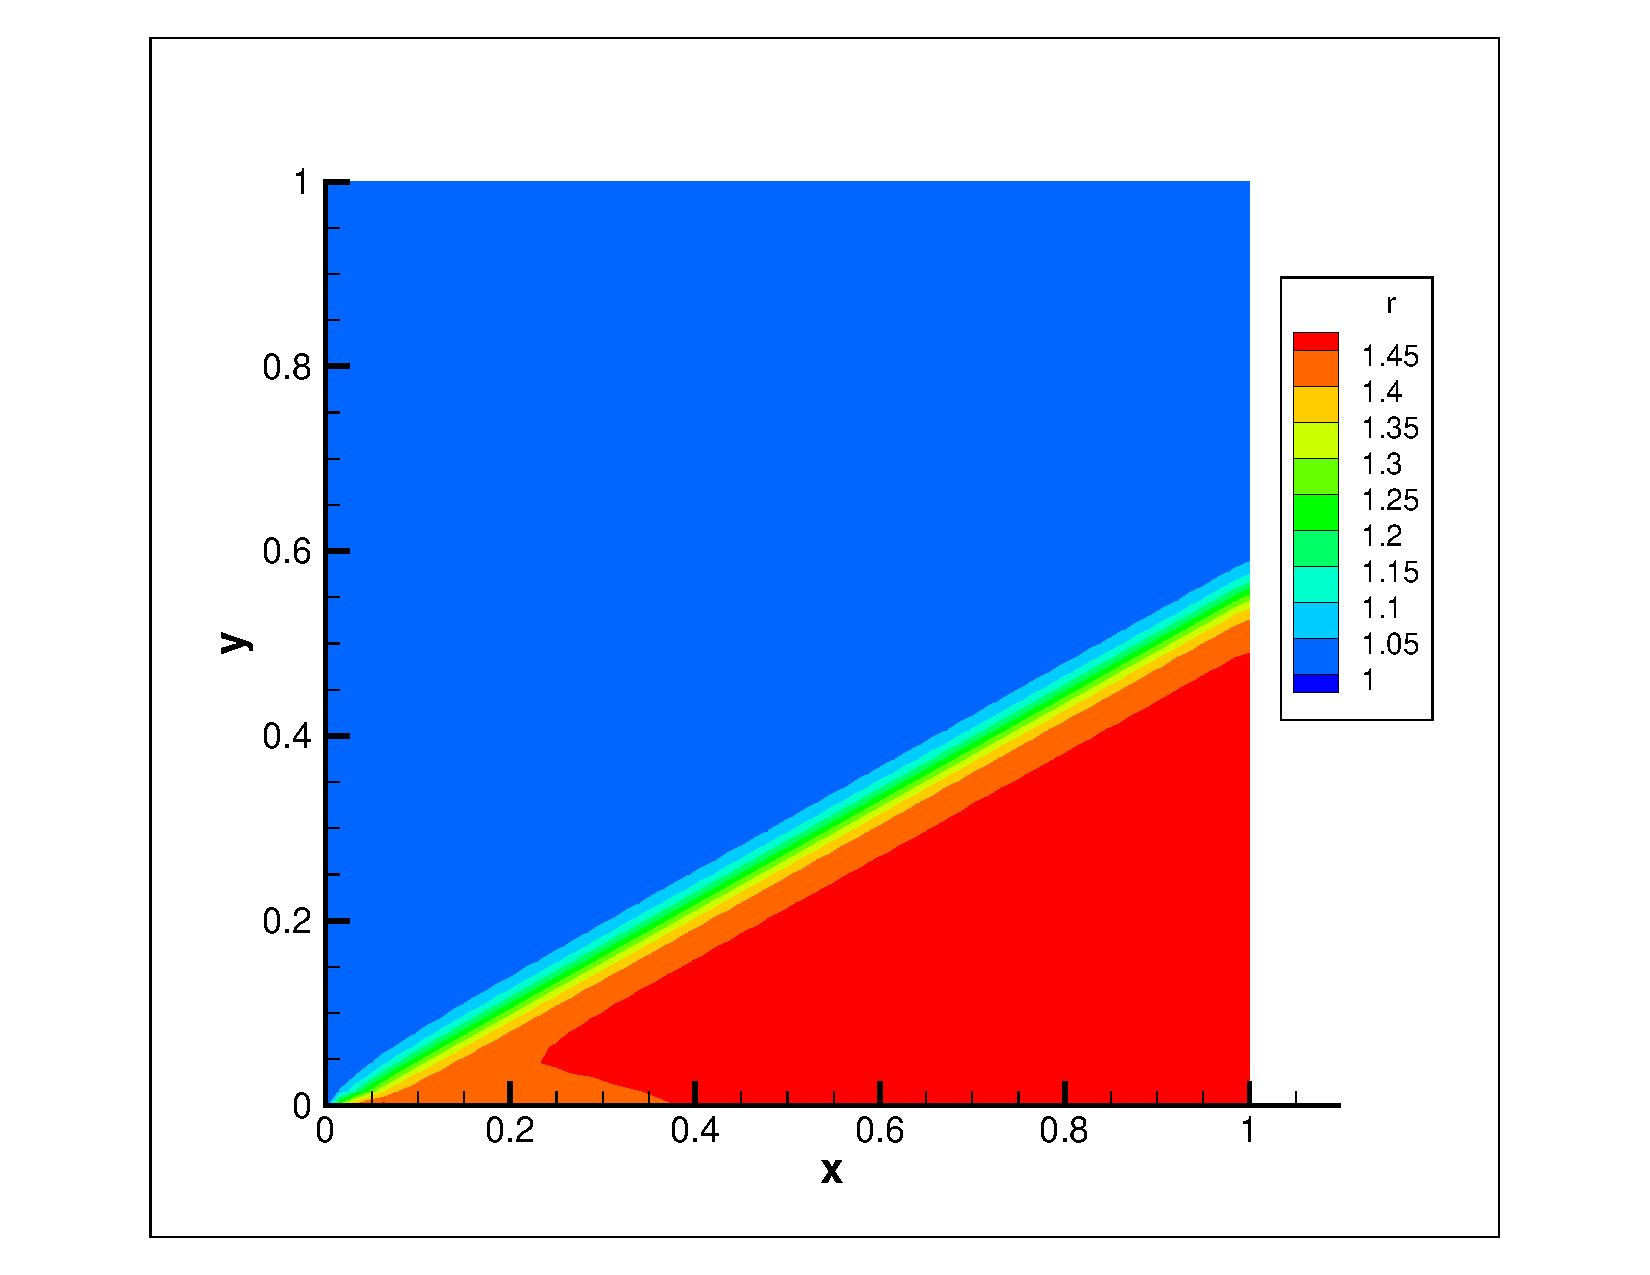
\includegraphics[viewport=110 30 600 520,clip=true,width=.42\textwidth]{fob_adapt_3_sol.pdf}}
        \end{center}
      \end{figure}
  \end{itemize}
}

\frame
{
  \frametitle{Redistributed Solutions}
  \begin{itemize}[<+->]
    \item Redistribution utilizing the same flux jump indicator.
      \begin{figure}[!htb]
        \begin{center}
          \subfigure[Mesh, 8 redistribution steps]{\label{fig:fob_redist_adapt_8_mesh}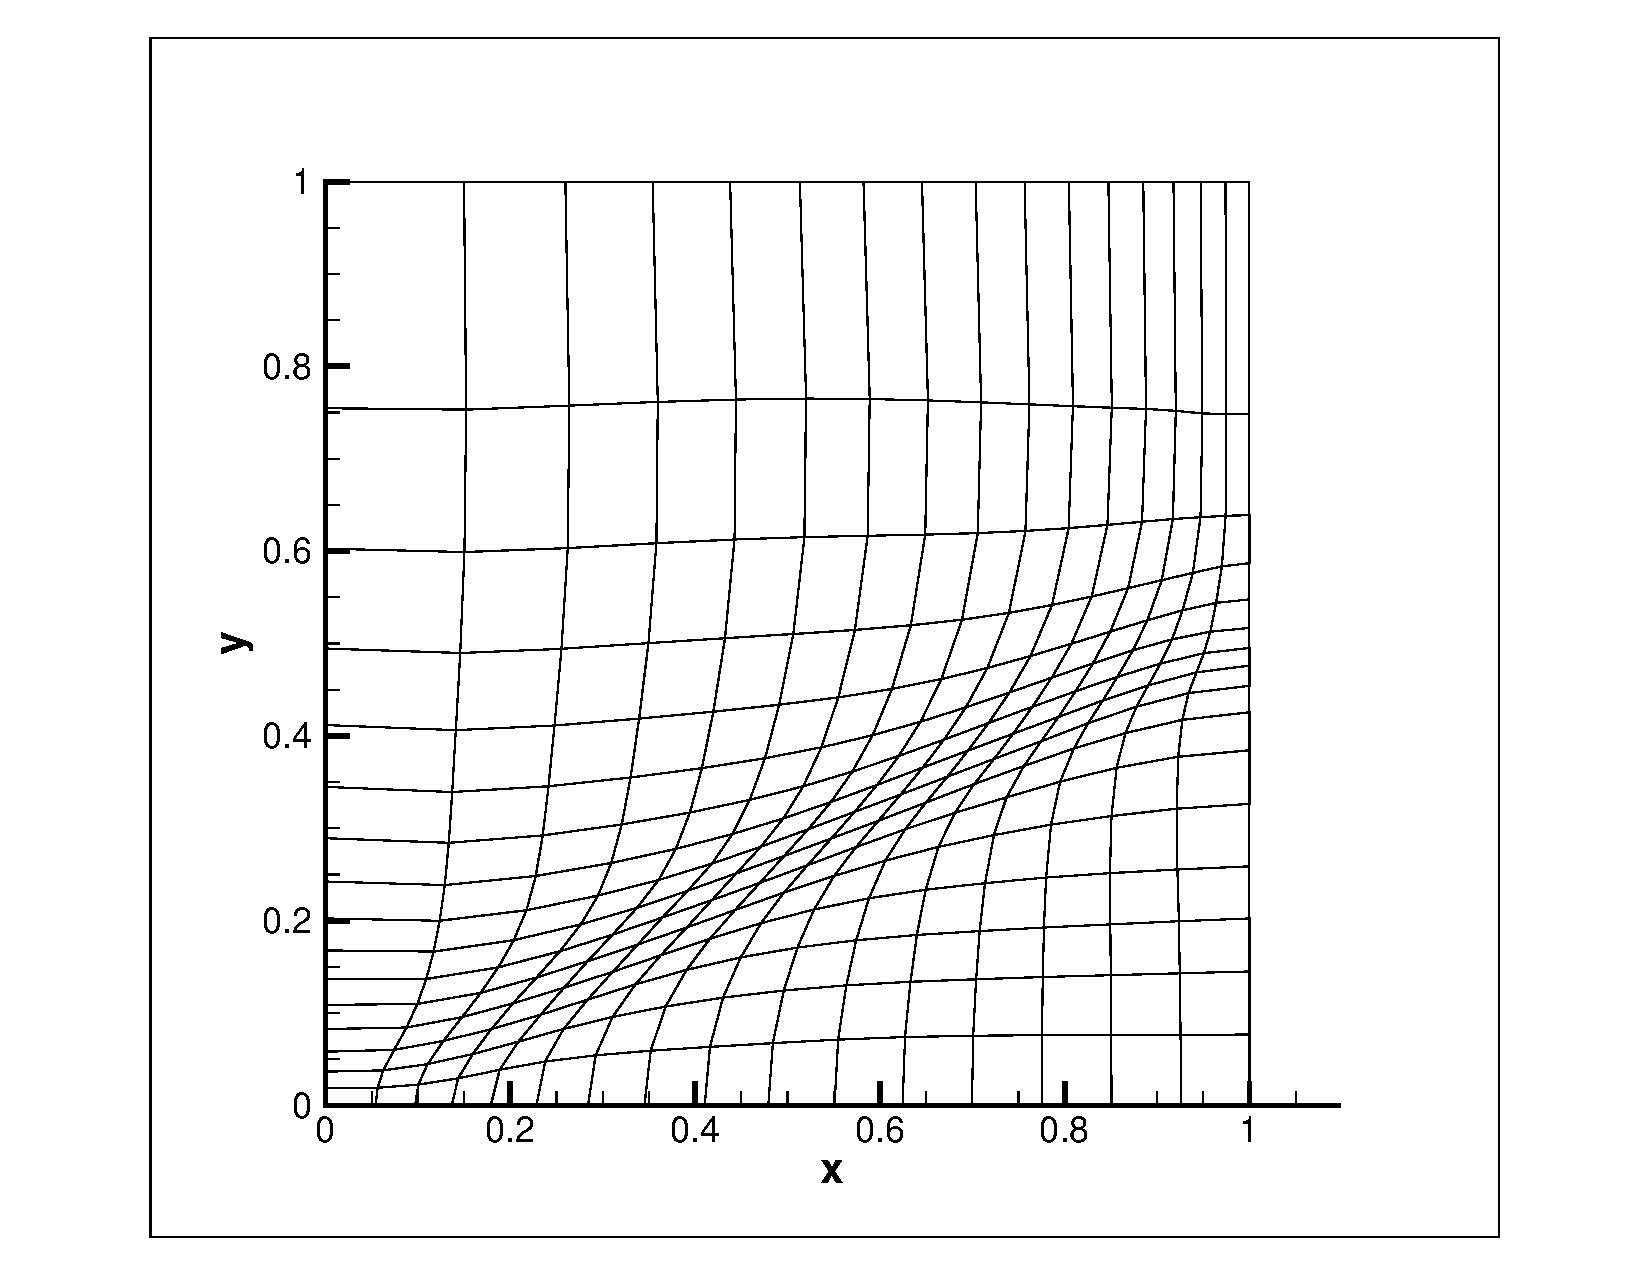
\includegraphics[viewport=110 30 600 550,clip=true,width=.42\textwidth]{fob_redist_adapt_8_mesh.pdf}}
          \subfigure[Solution]{\label{fig:fob_redist_adapt_8_sol}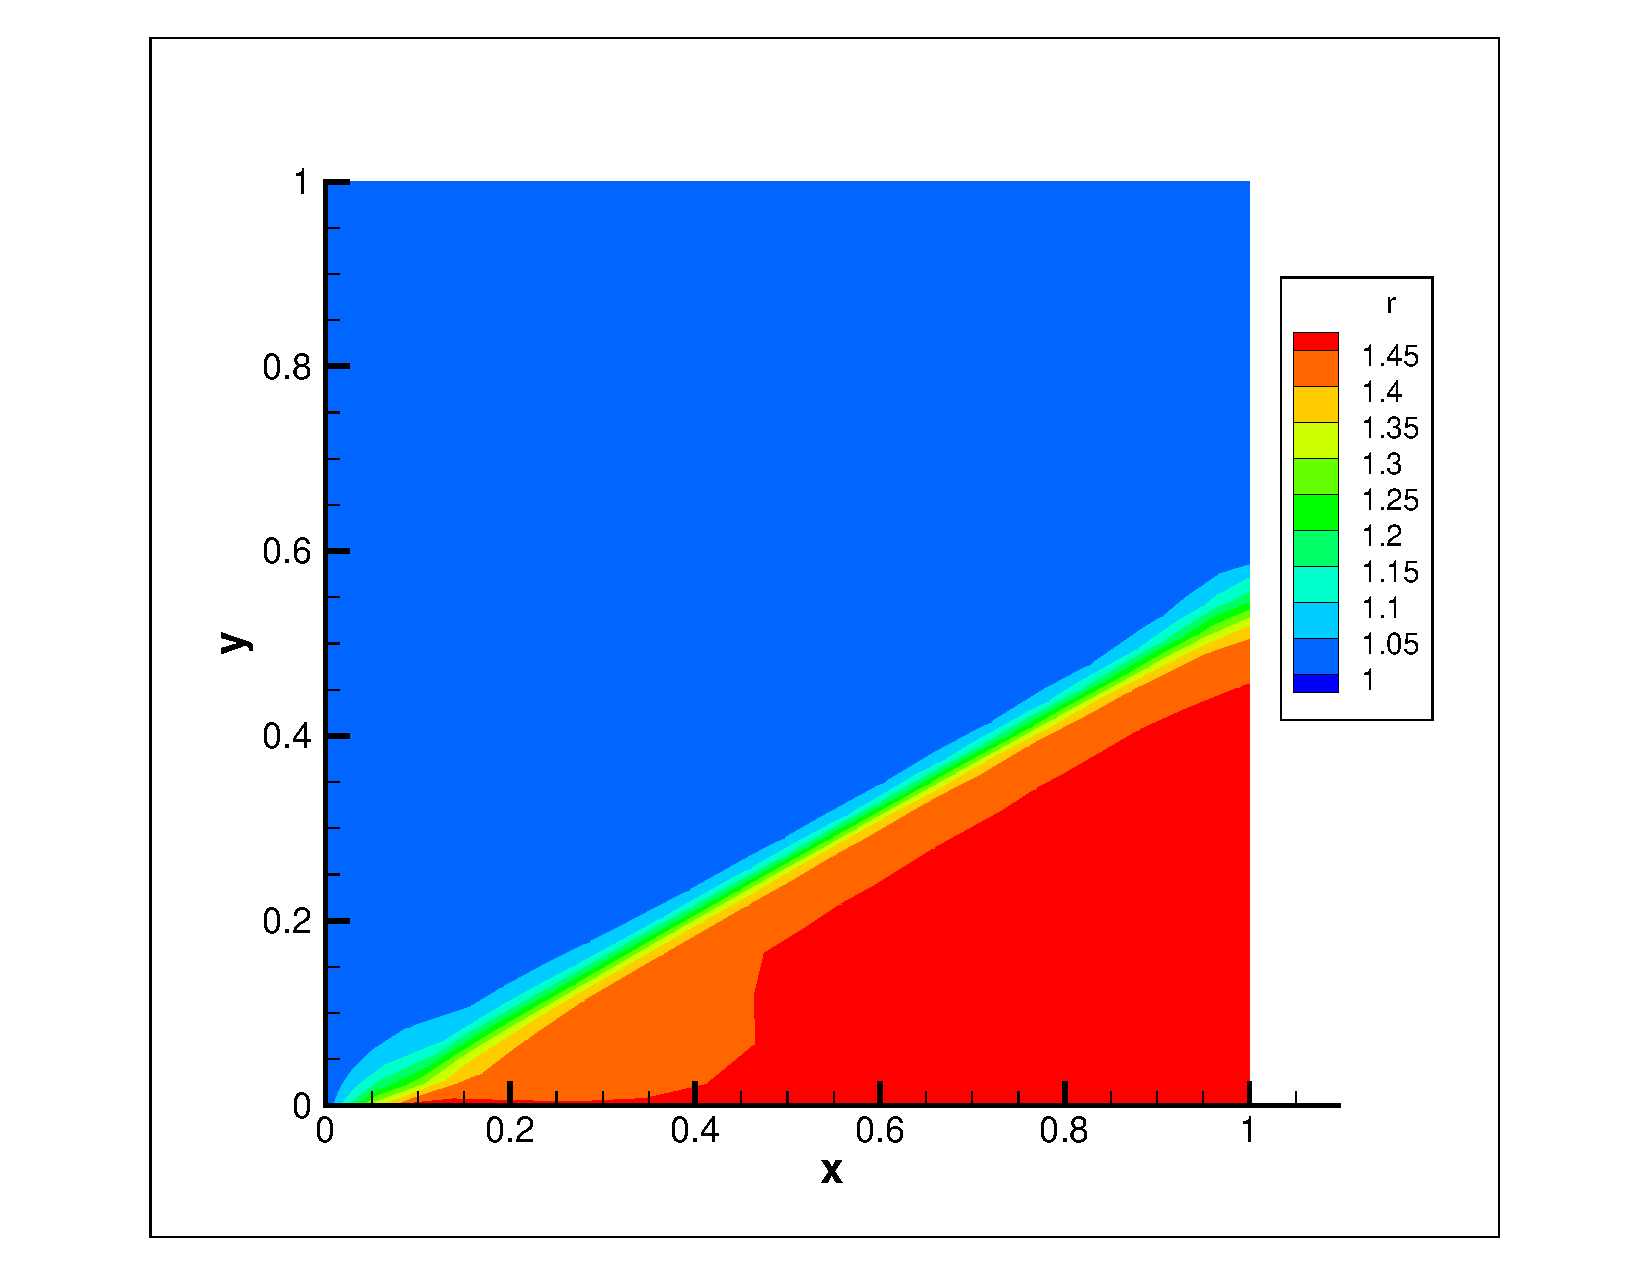
\includegraphics[viewport=110 30 600 520,clip=true,width=.42\textwidth]{fob_redist_adapt_8_sol.pdf}}
        \end{center}
      \end{figure}
  \end{itemize}
}

\frame
{
  \frametitle{Redistributed and Adapted}
  \begin{itemize}[<+->]
    \item Now combining the two, here are the mesh and solution after 2 adaptations beyond the previous redistribution containing 10190 DOFs.
      \begin{figure}[!htb]
        \begin{center}
          \subfigure[Mesh, 2 refinements]{\label{fig:fob_redist_adapt_10_mesh}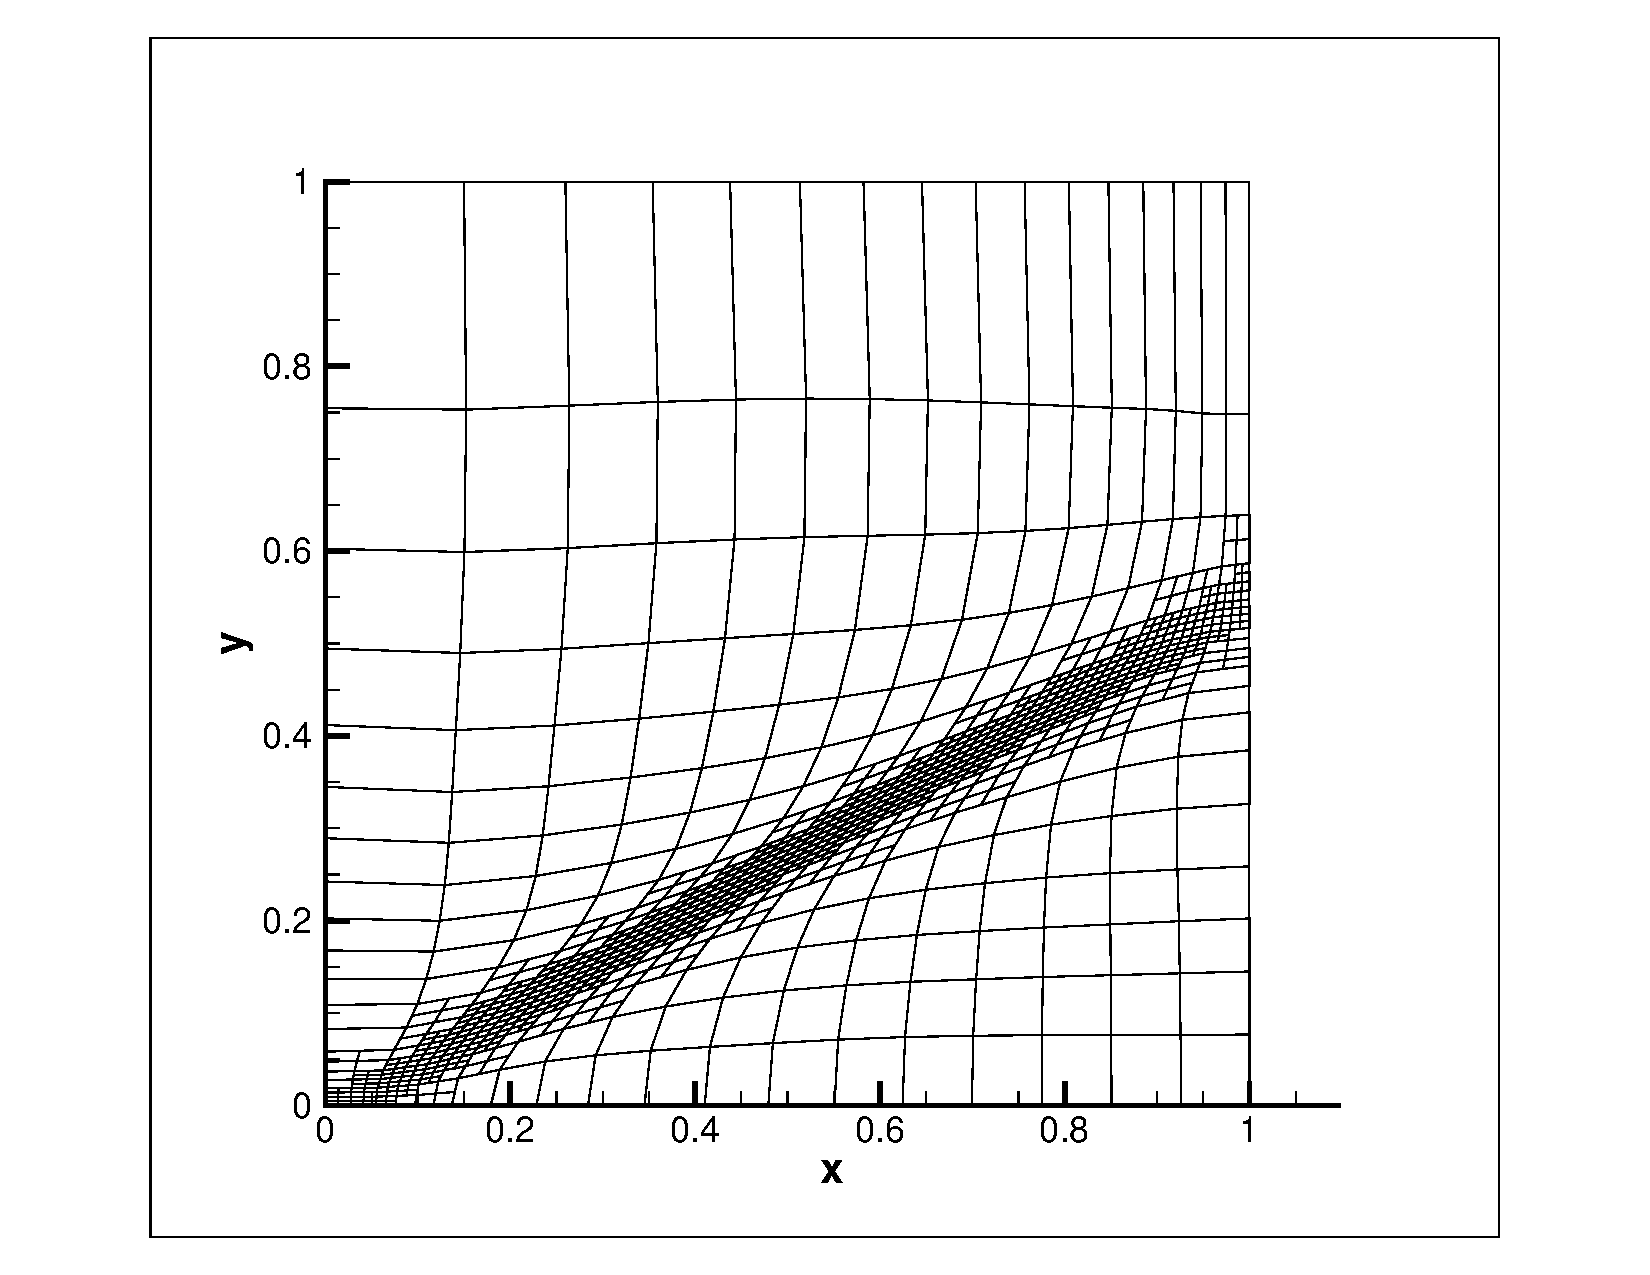
\includegraphics[viewport=110 30 600 550,clip=true,width=.42\textwidth]{fob_redist_adapt_10_mesh.pdf}}
          \subfigure[Solution]{\label{fig:fob_redist_adapt_10_sol}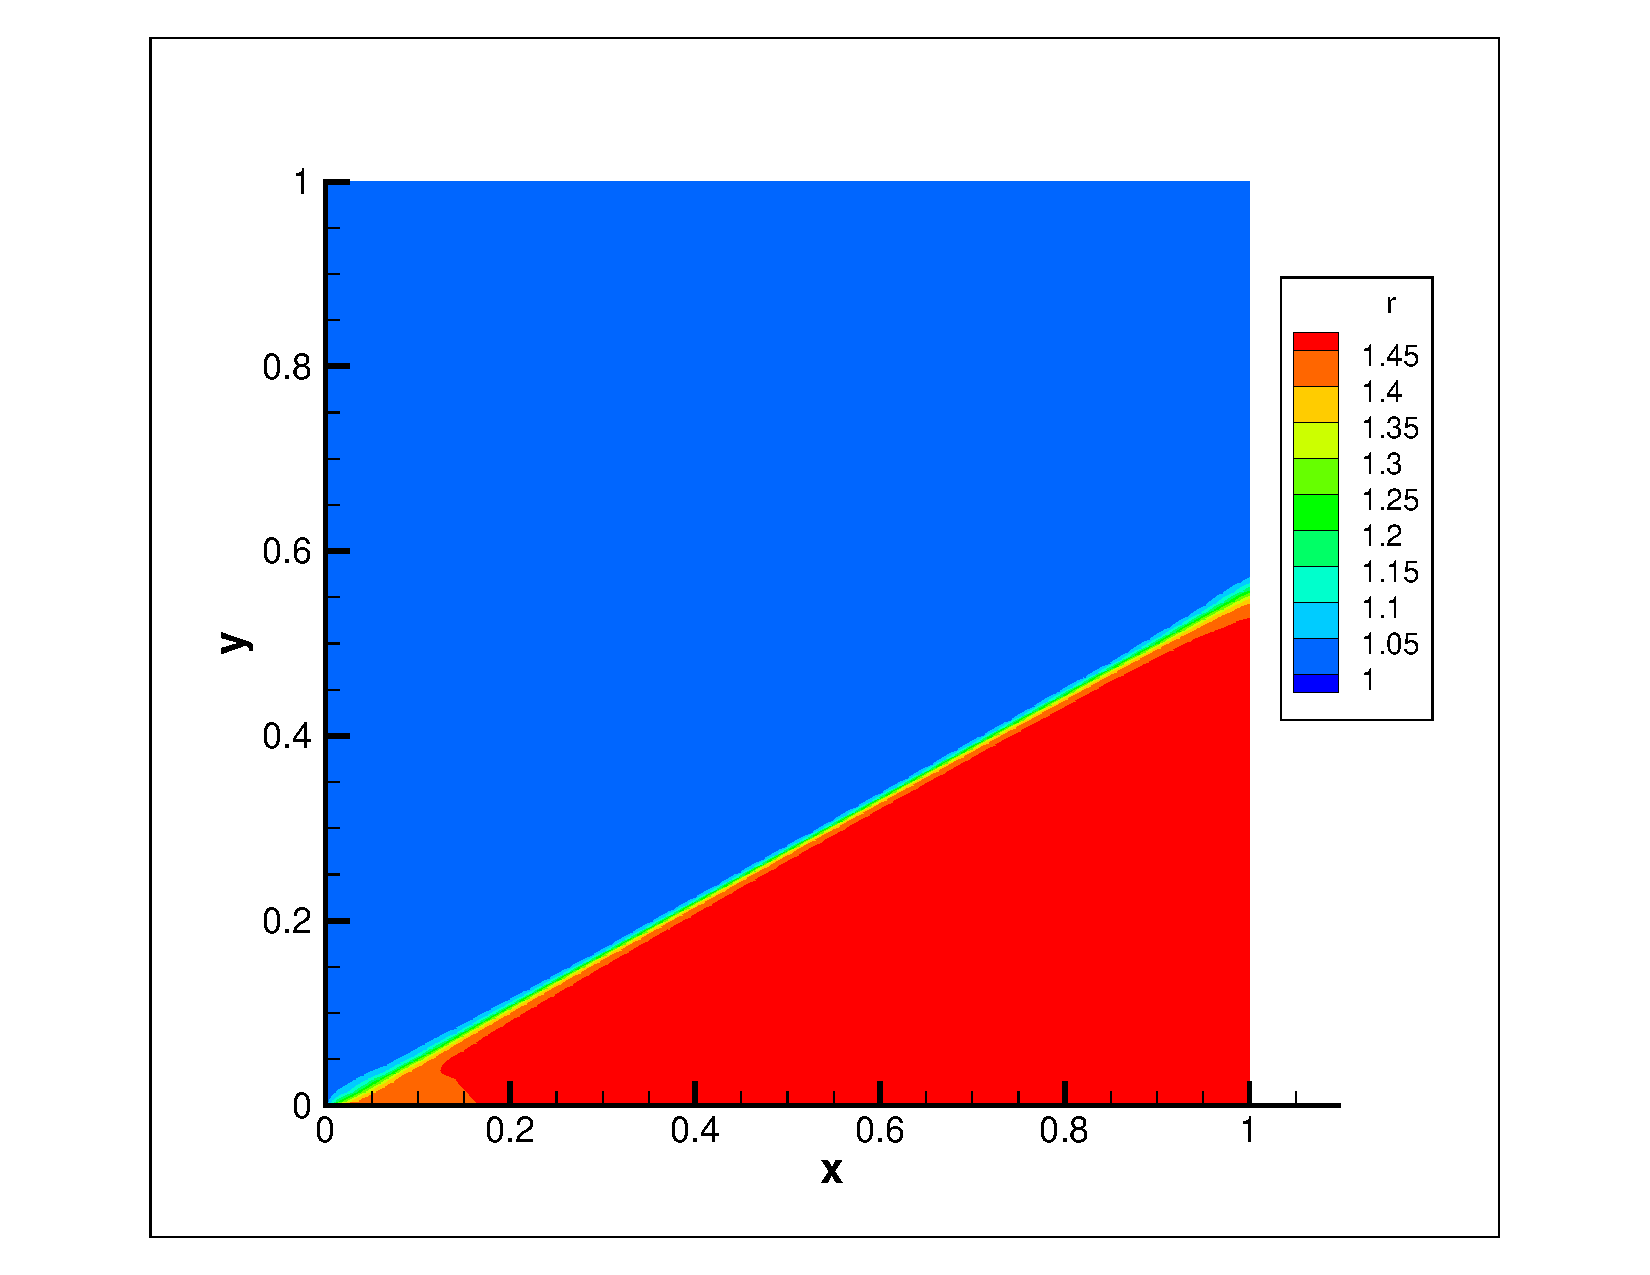
\includegraphics[viewport=110 30 600 520,clip=true,width=.42\textwidth]{fob_redist_adapt_10_sol.pdf}}
        \end{center}
      \end{figure}
  \end{itemize}
}

\frame
{
  \frametitle{Solution Comparison}
  \begin{itemize}[<+->]
    \item For a better comparison here are 3 of the solutions, each with around 11000 DOFs:
      \begin{figure}[!htb]
        \begin{center}
          \subfigure[Uniform.]{\label{fig:fob_uniform_2_sol}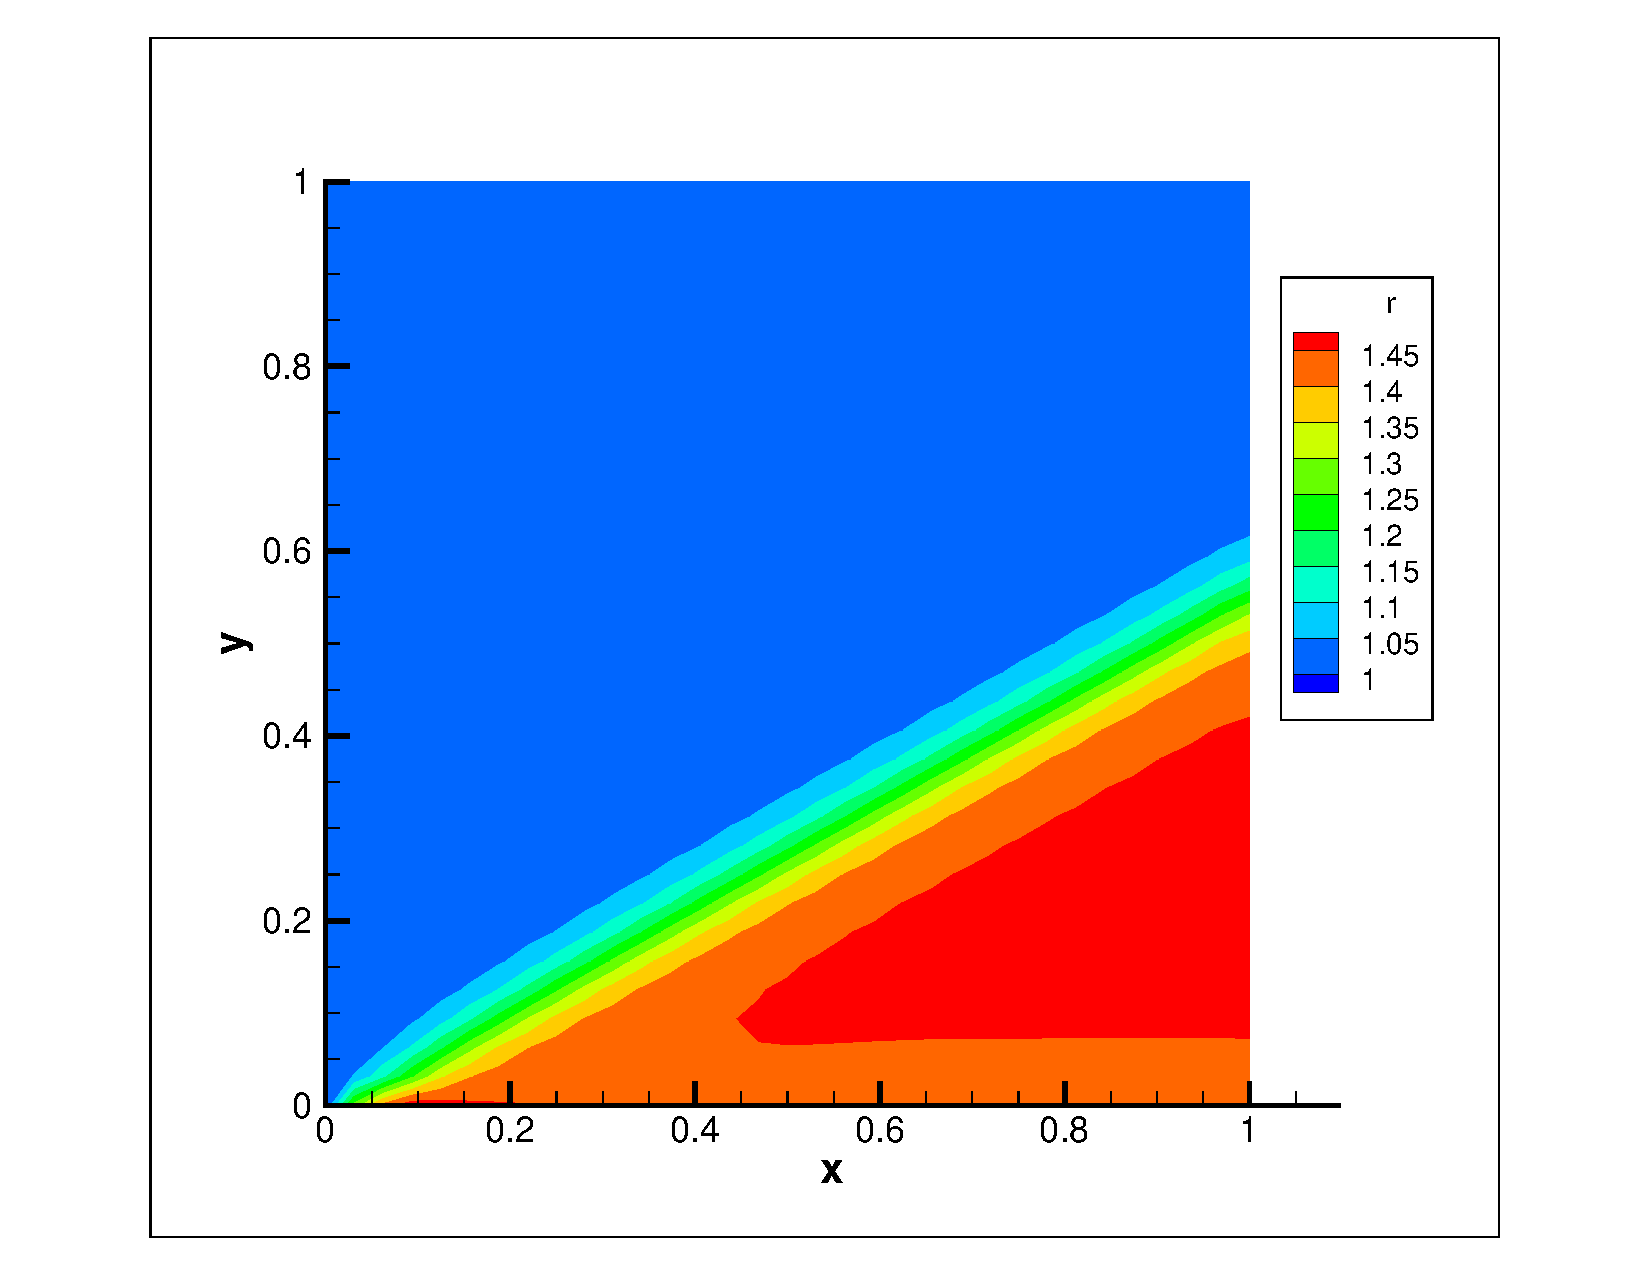
\includegraphics[viewport=110 30 600 520,clip=true,width=.3\textwidth]{fob_uniform_2_sol.pdf}}
          \subfigure[Adaptive.]{\label{fig:fob_adapt_3_sol}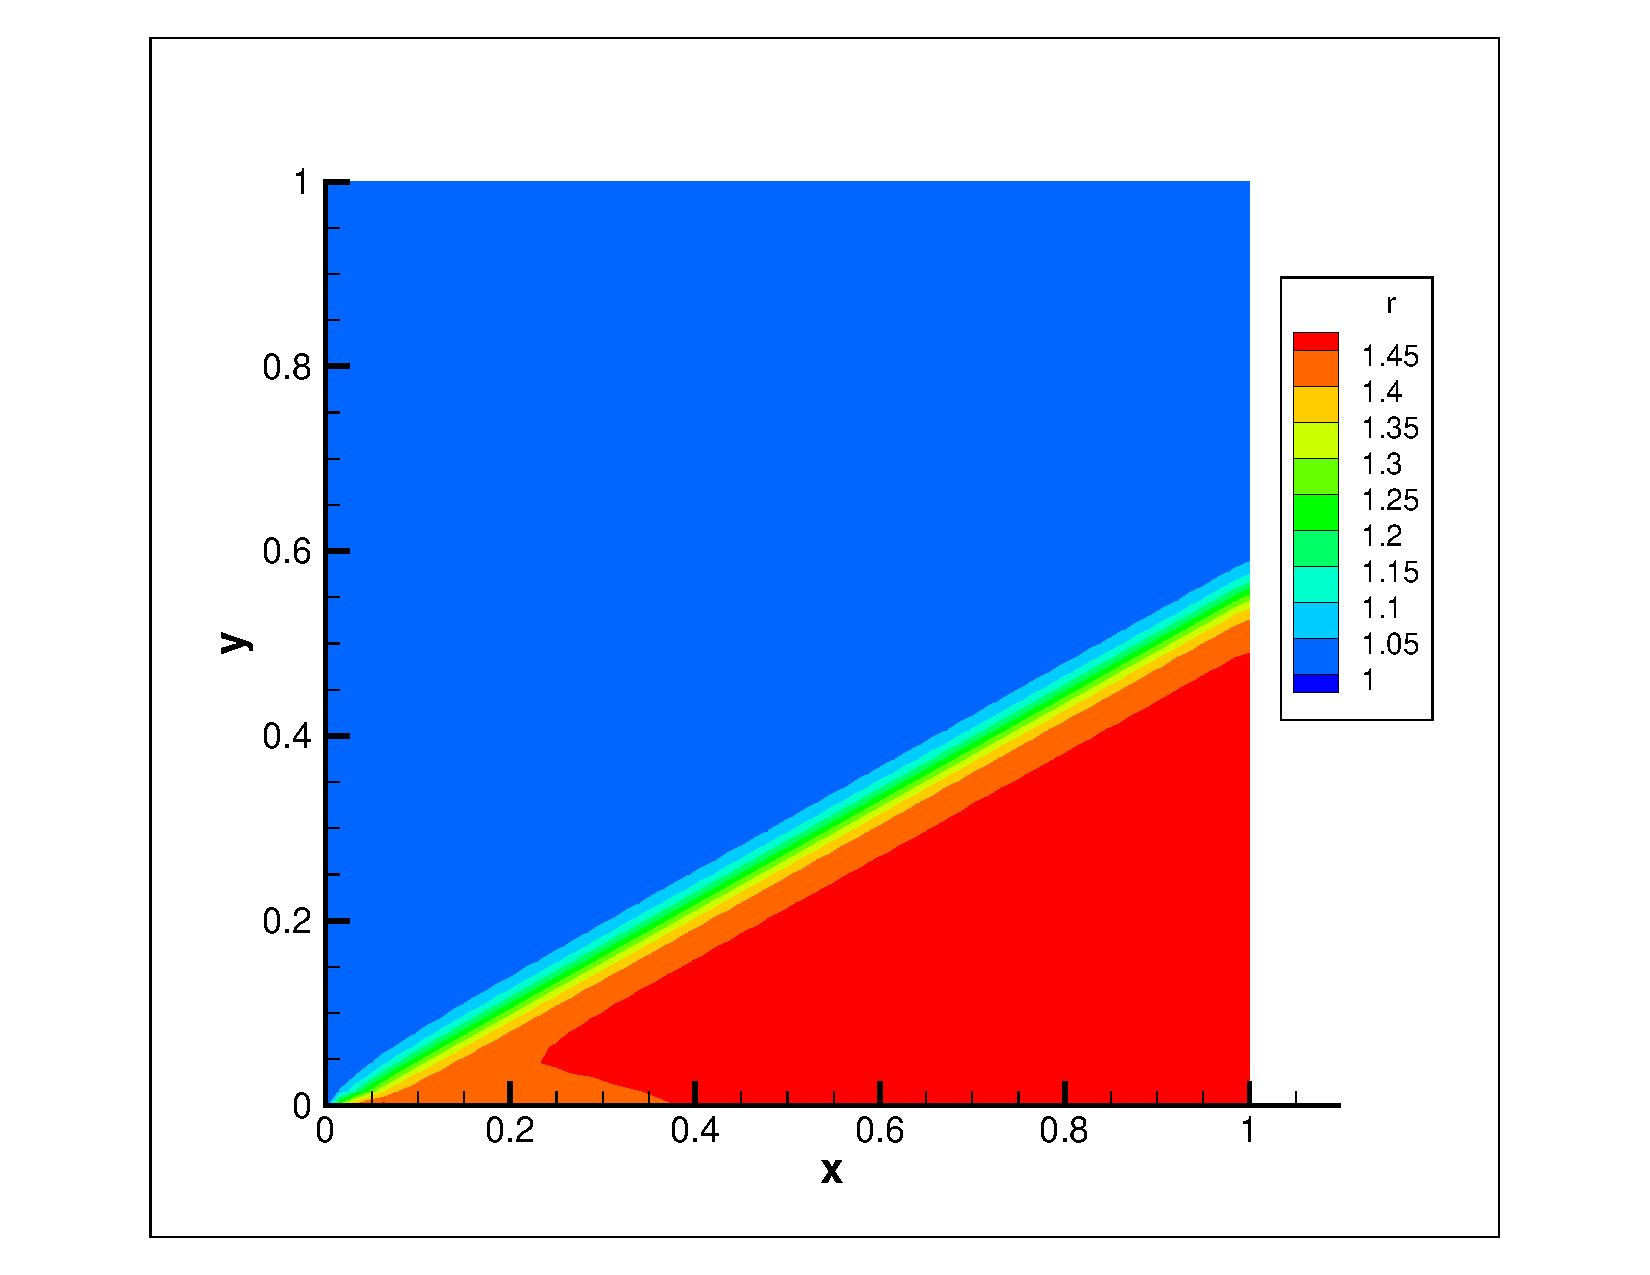
\includegraphics[viewport=110 30 600 520,clip=true,width=.3\textwidth]{fob_adapt_3_sol.pdf}}
          \subfigure[R + H.]{\label{fig:fob_redist_adapt_10_sol}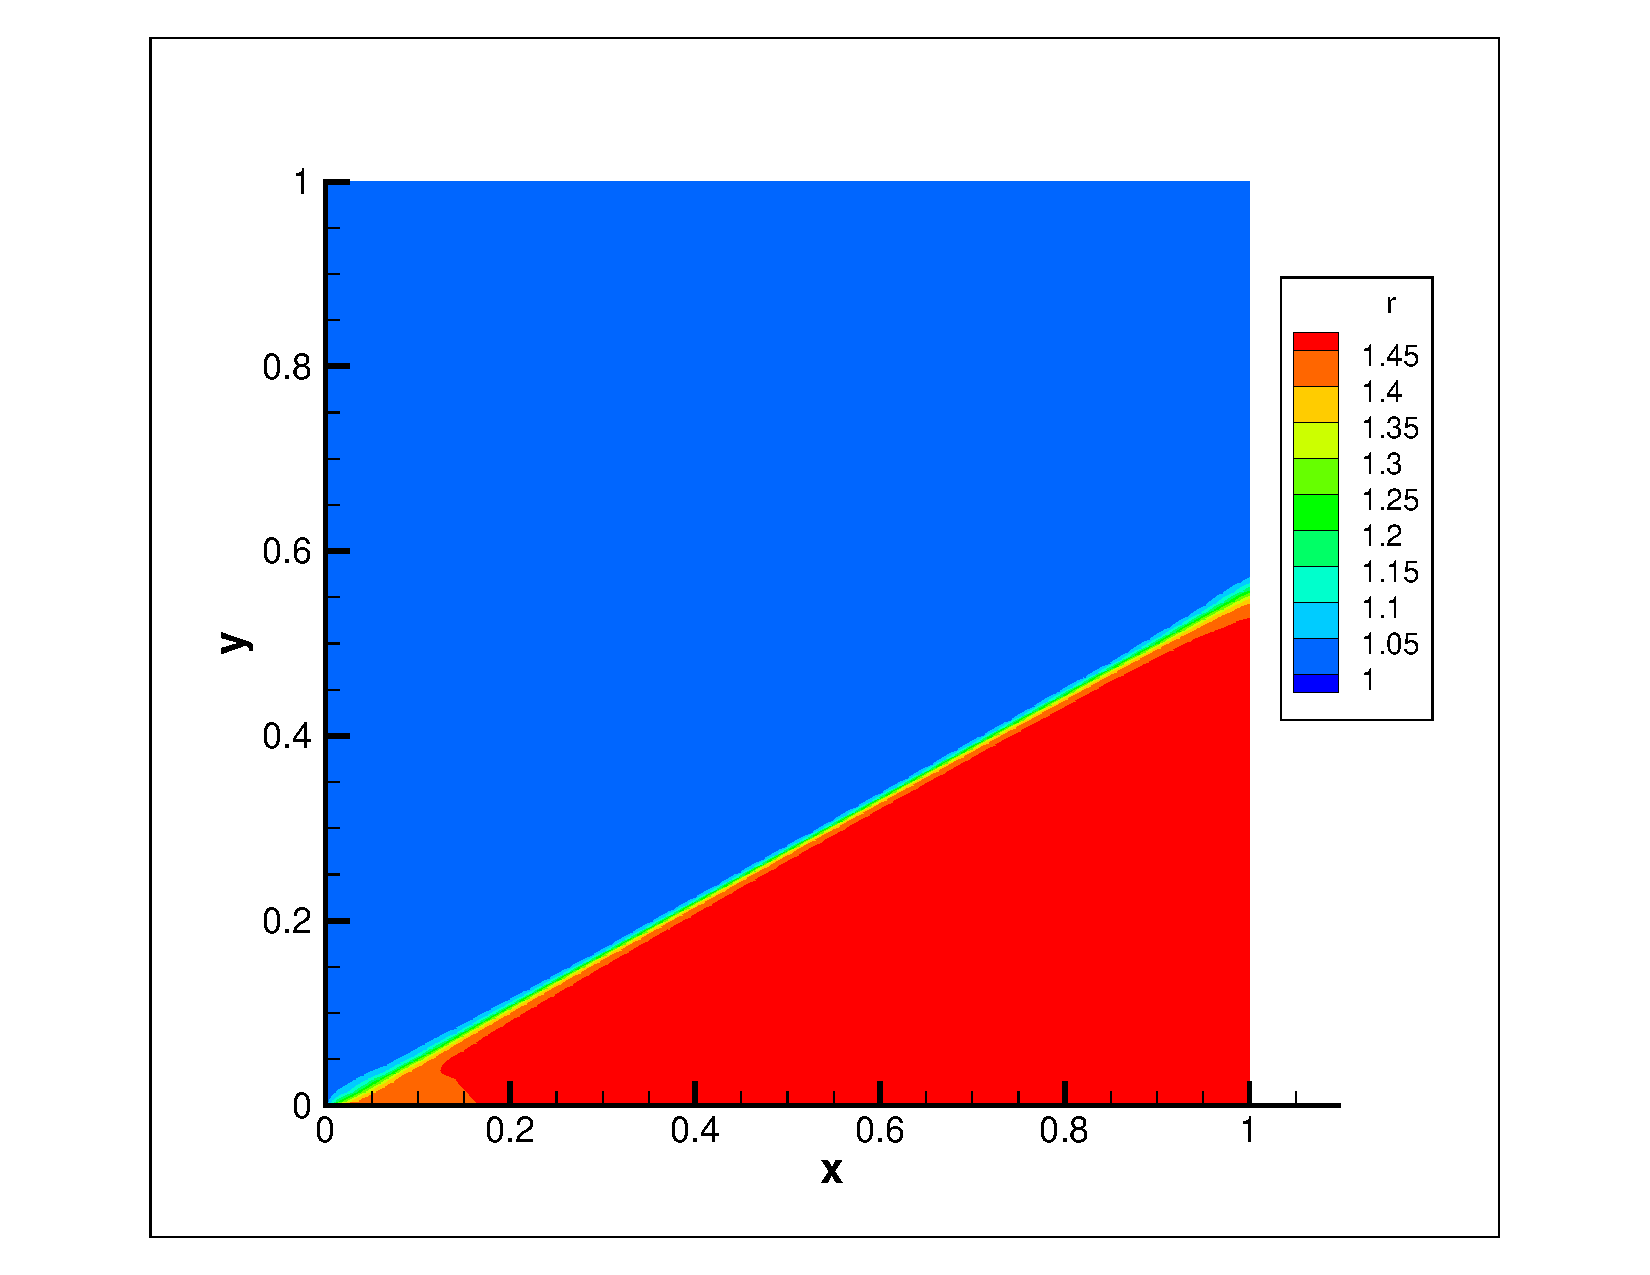
\includegraphics[viewport=110 30 600 520,clip=true,width=.3\textwidth]{fob_redist_adapt_10_sol.pdf}}
        \end{center}
      \end{figure}
  \end{itemize}
}

\frame
{
  \frametitle{Error Plot}
  \begin{itemize}[<+->]
    \item libmesh provides capability for computing error norms against an exact solution.
    \item The exact solution is not in $H^1$ therefore we only obtain
the $L_2$ convergence plot:
      \begin{figure}[!htb]
      \begin{center}
        \subfigure[LogLog plot of L2 vs DOFs.]{\label{fig:fob_l2}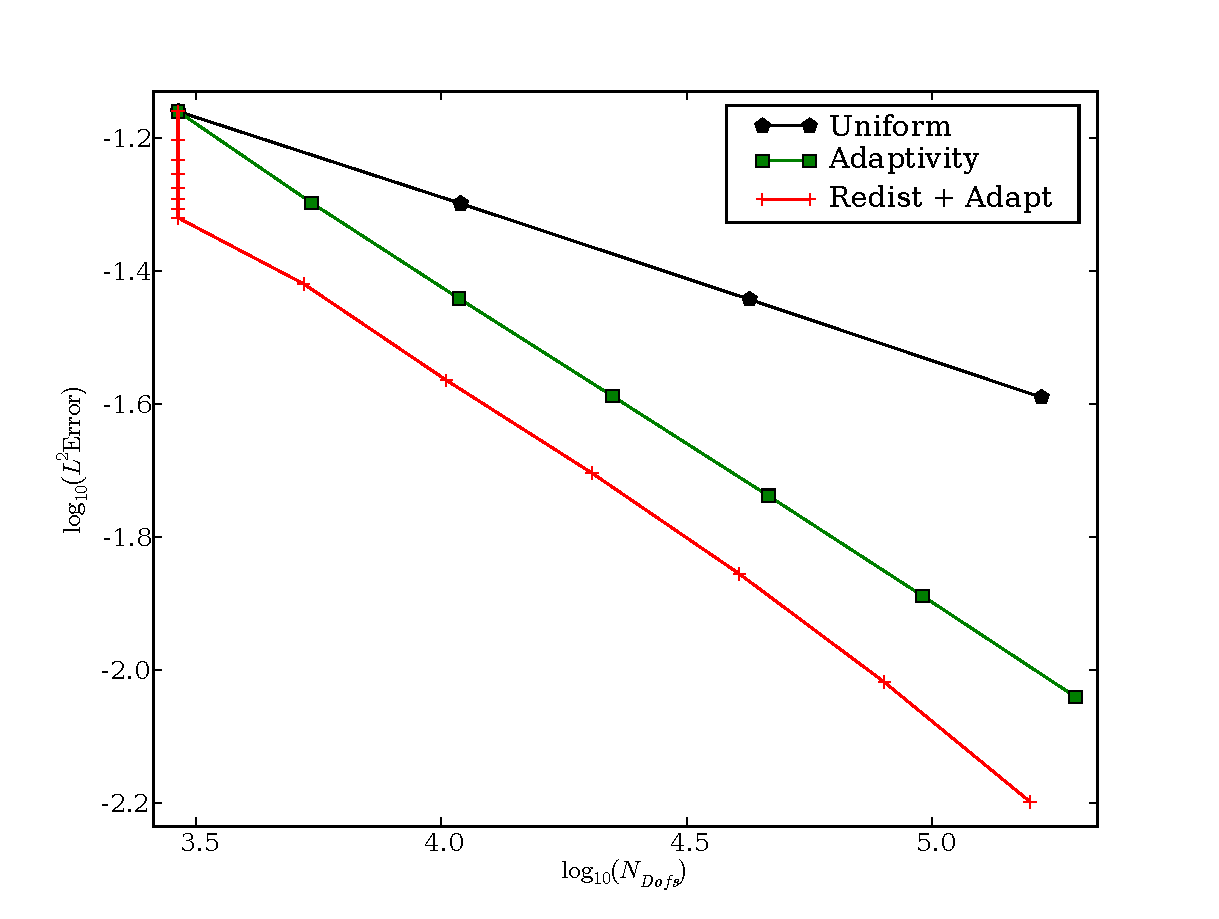
\includegraphics[viewport=0 10 600 400,clip=true,width=.7\textwidth]{fob_l2.pdf}}
      \end{center}
      \end{figure}
  \end{itemize}
}

\frame
{
  %\frametitle{Other Compressible Flow Examples}
    \begin{figure}[!htb]
      \begin{center}
        \subfigure{\label{fig:fob_uniform_2_sol}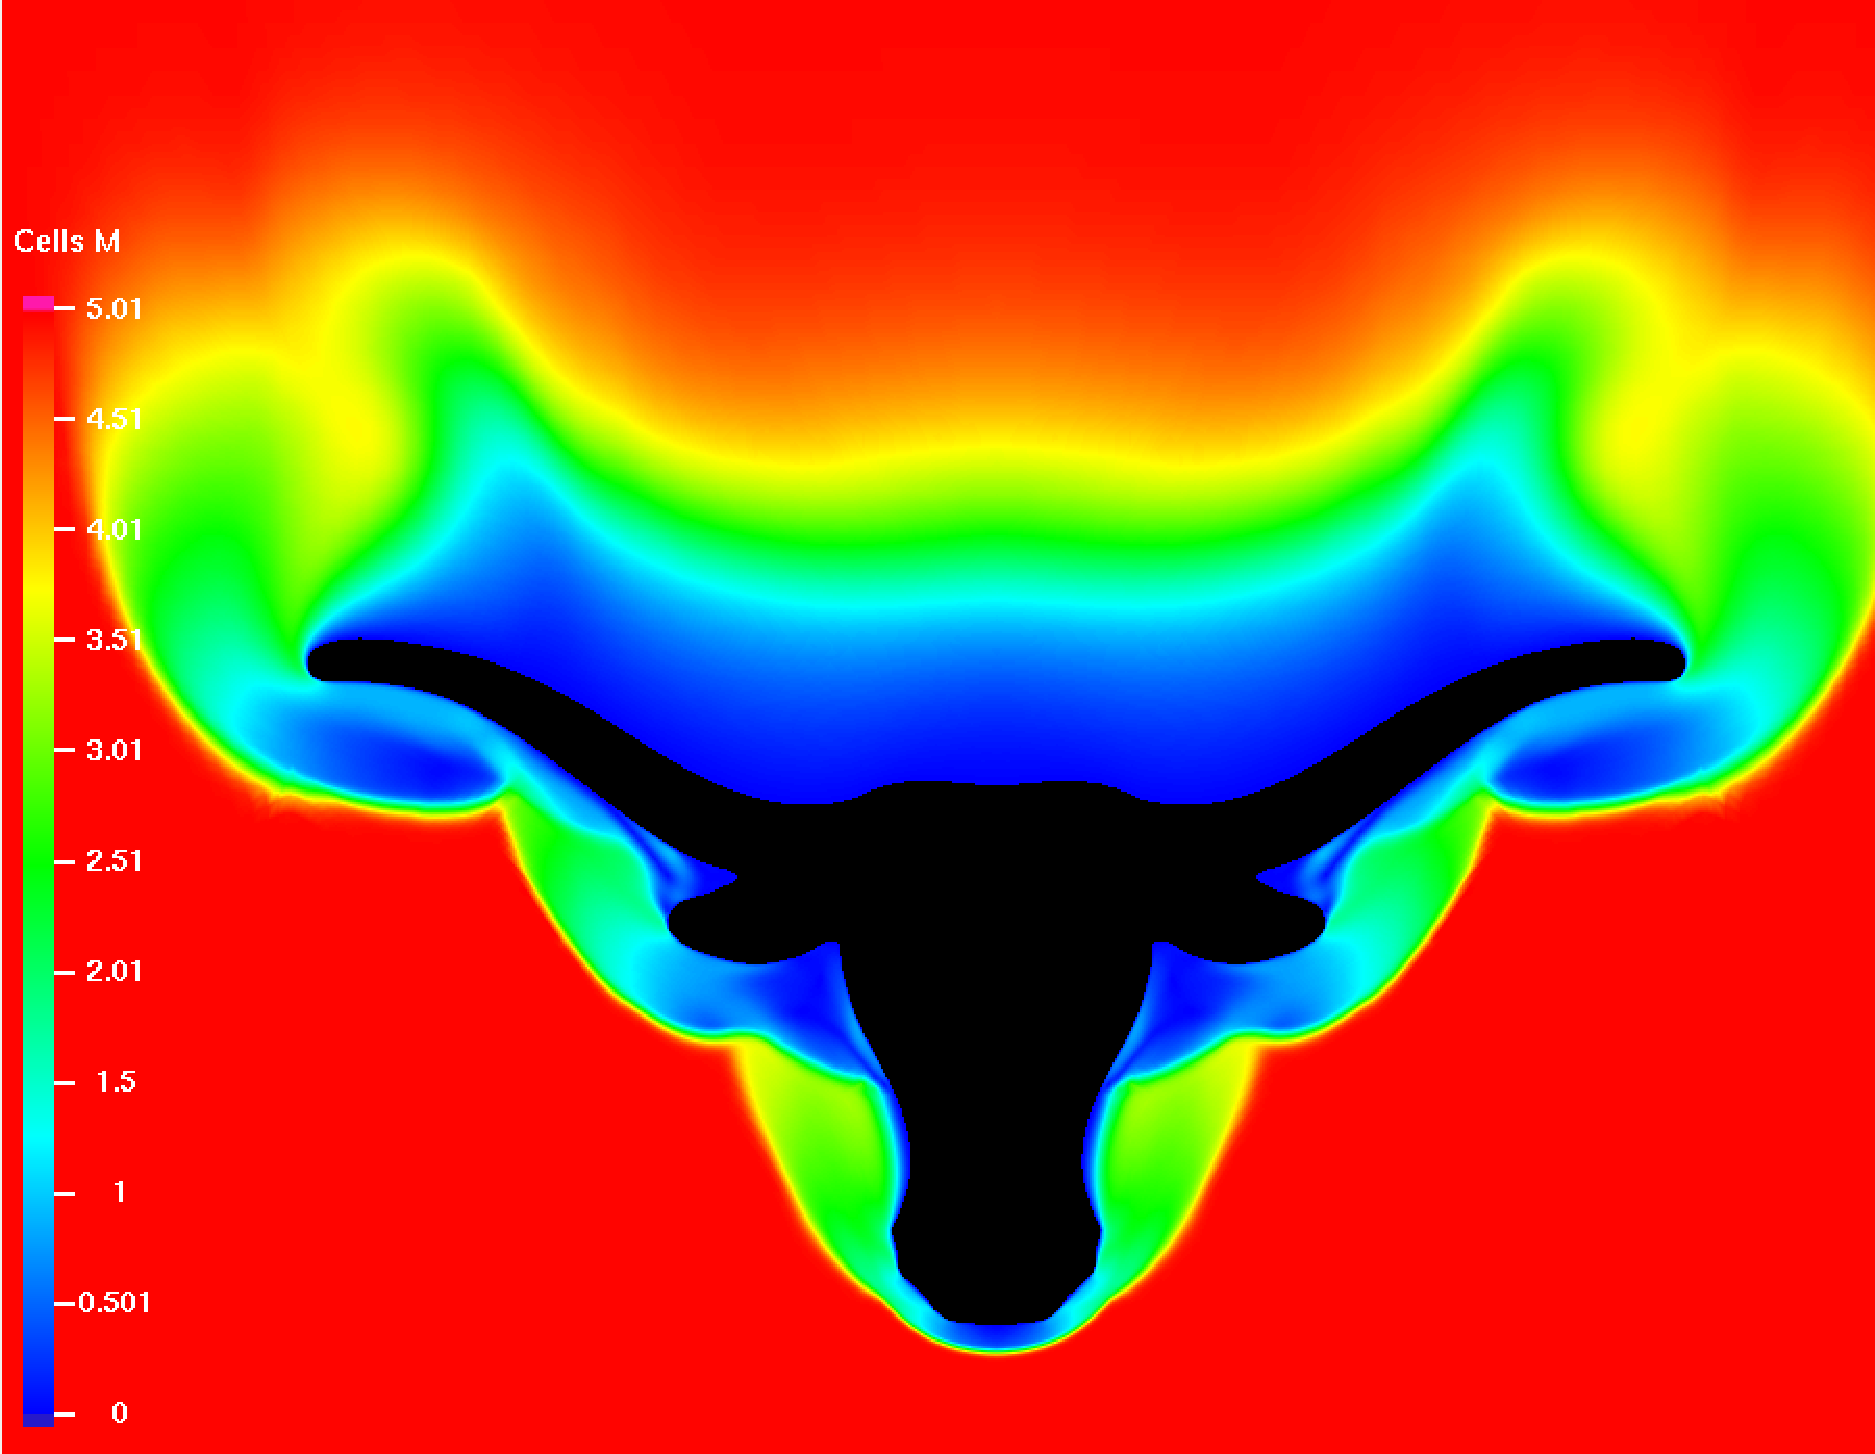
\includegraphics[width=.4\textwidth]{Hypersonic_cow_mach}}
        \subfigure{\label{fig:fob_adapt_3_sol}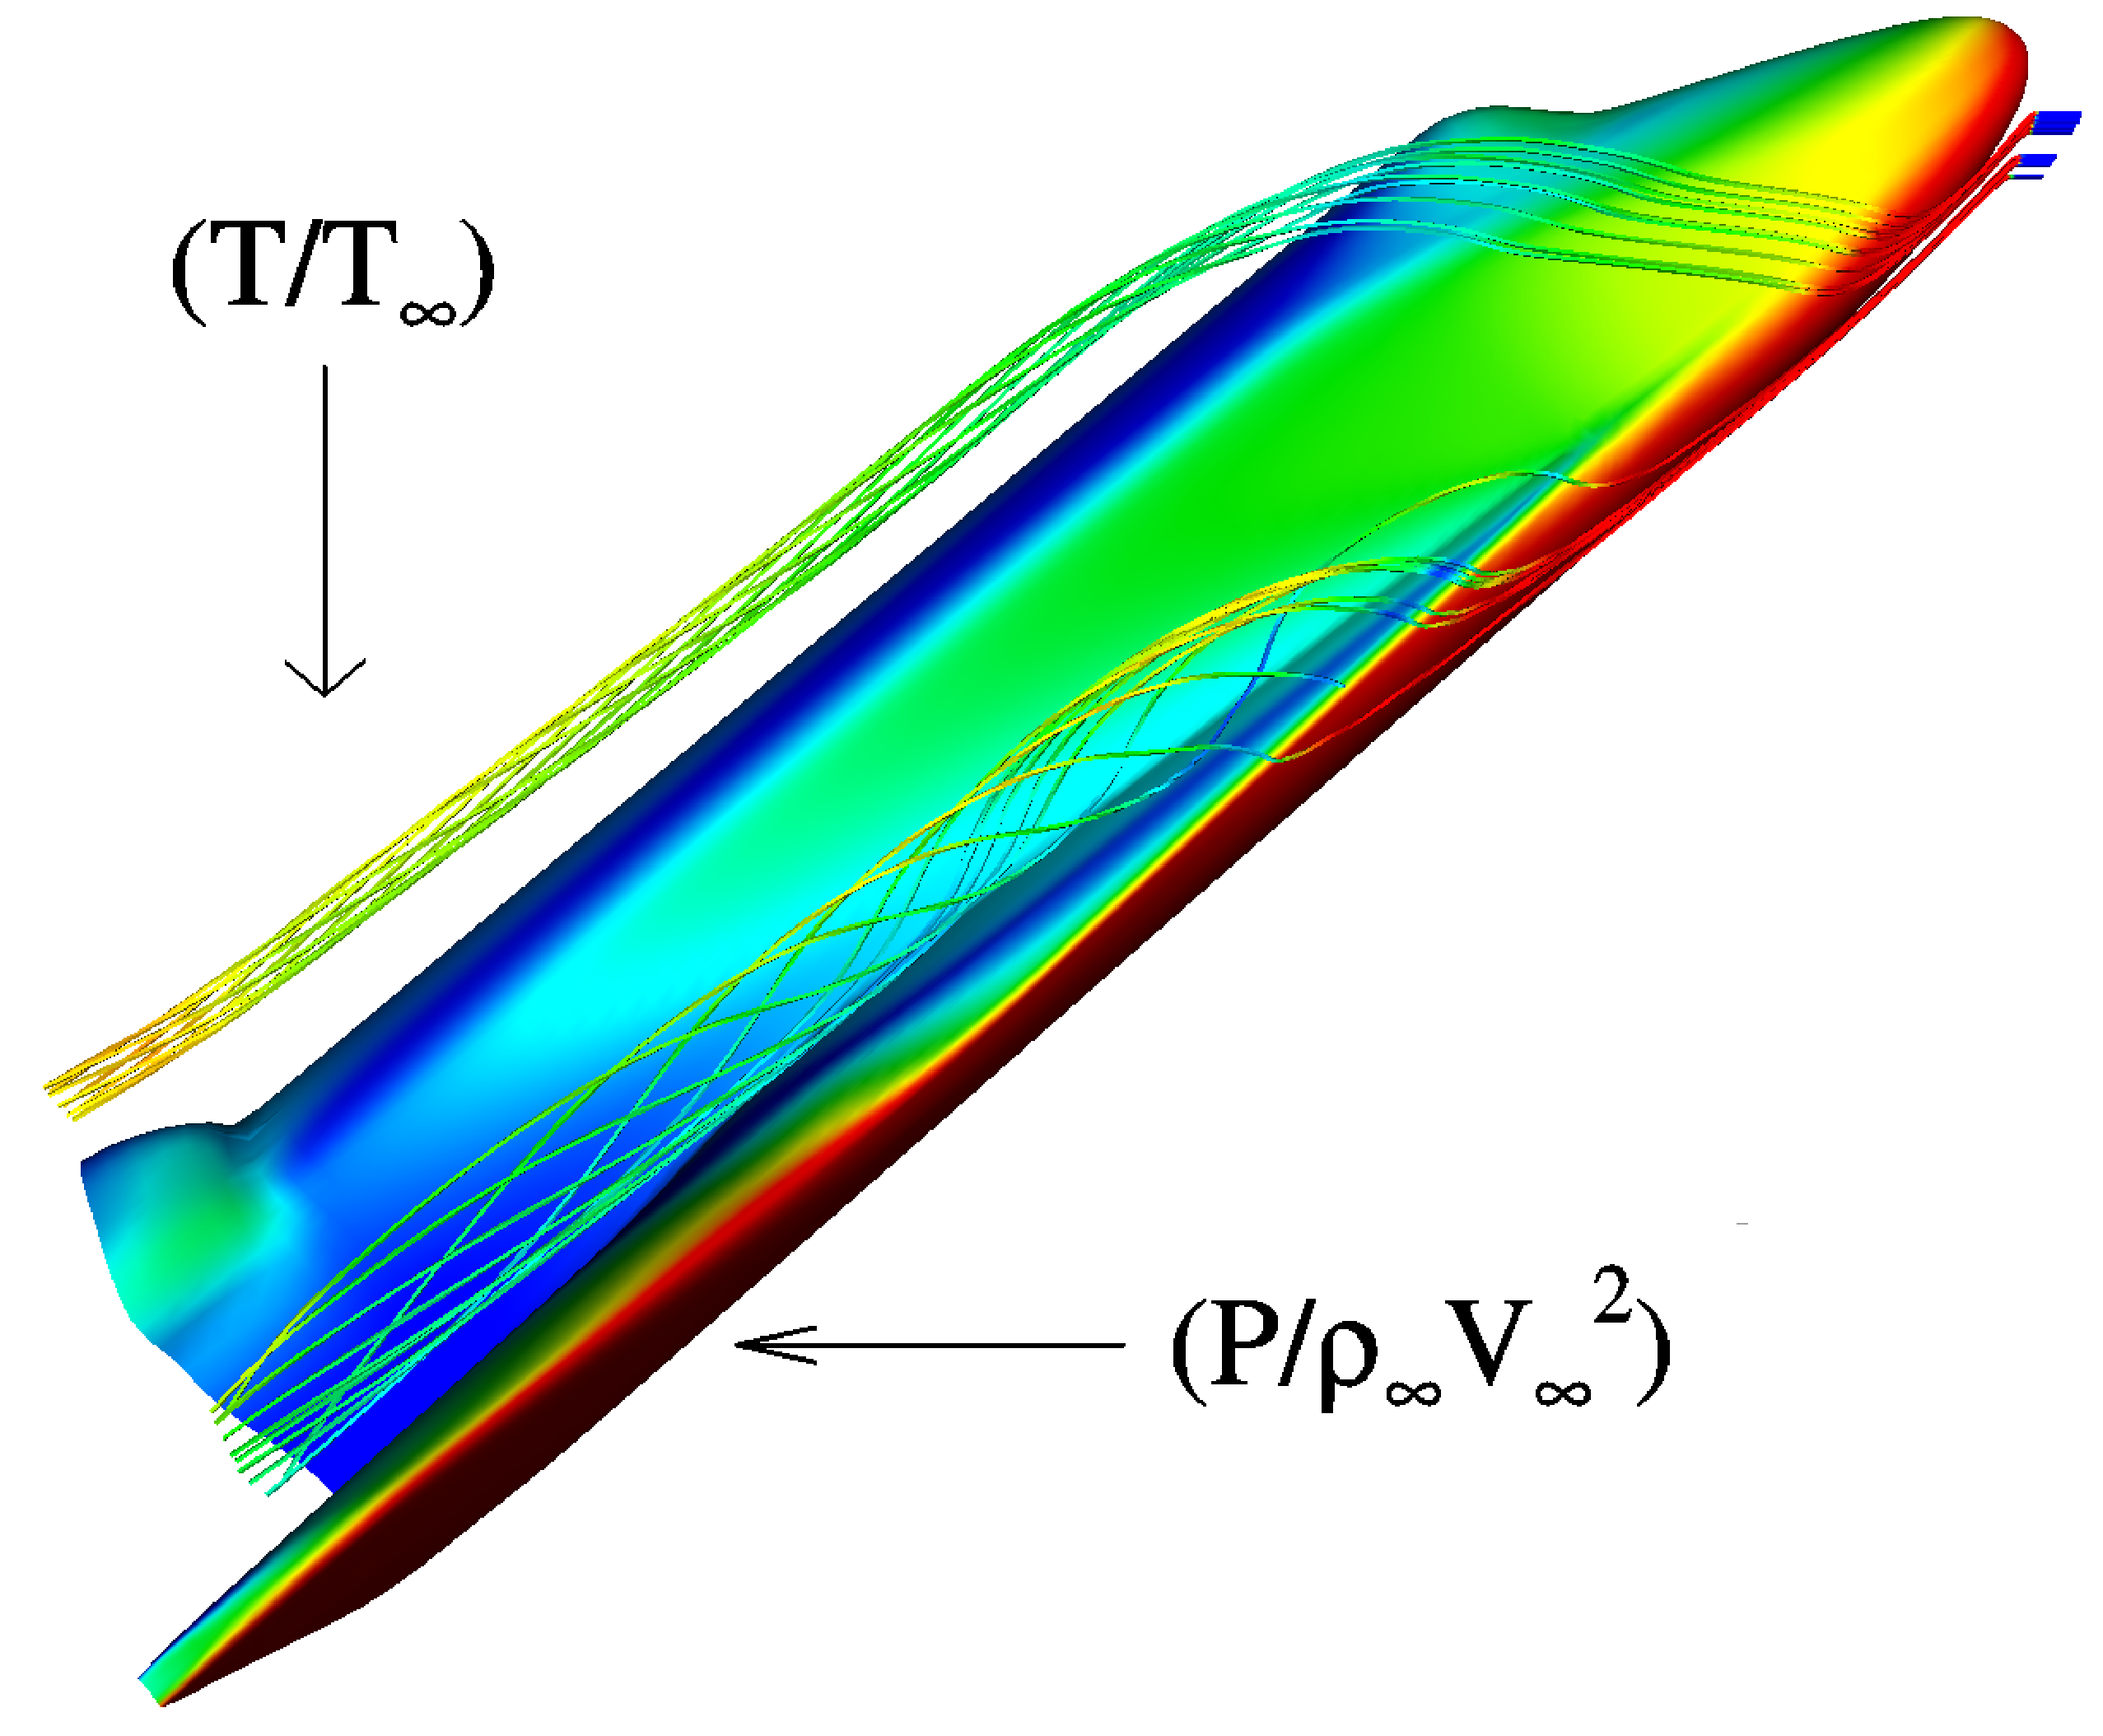
\includegraphics[width=.4\textwidth]{Benkirk_orbiter_reentry_side_view}}
        \subfigure{\label{fig:fob_redist_adapt_10_sol}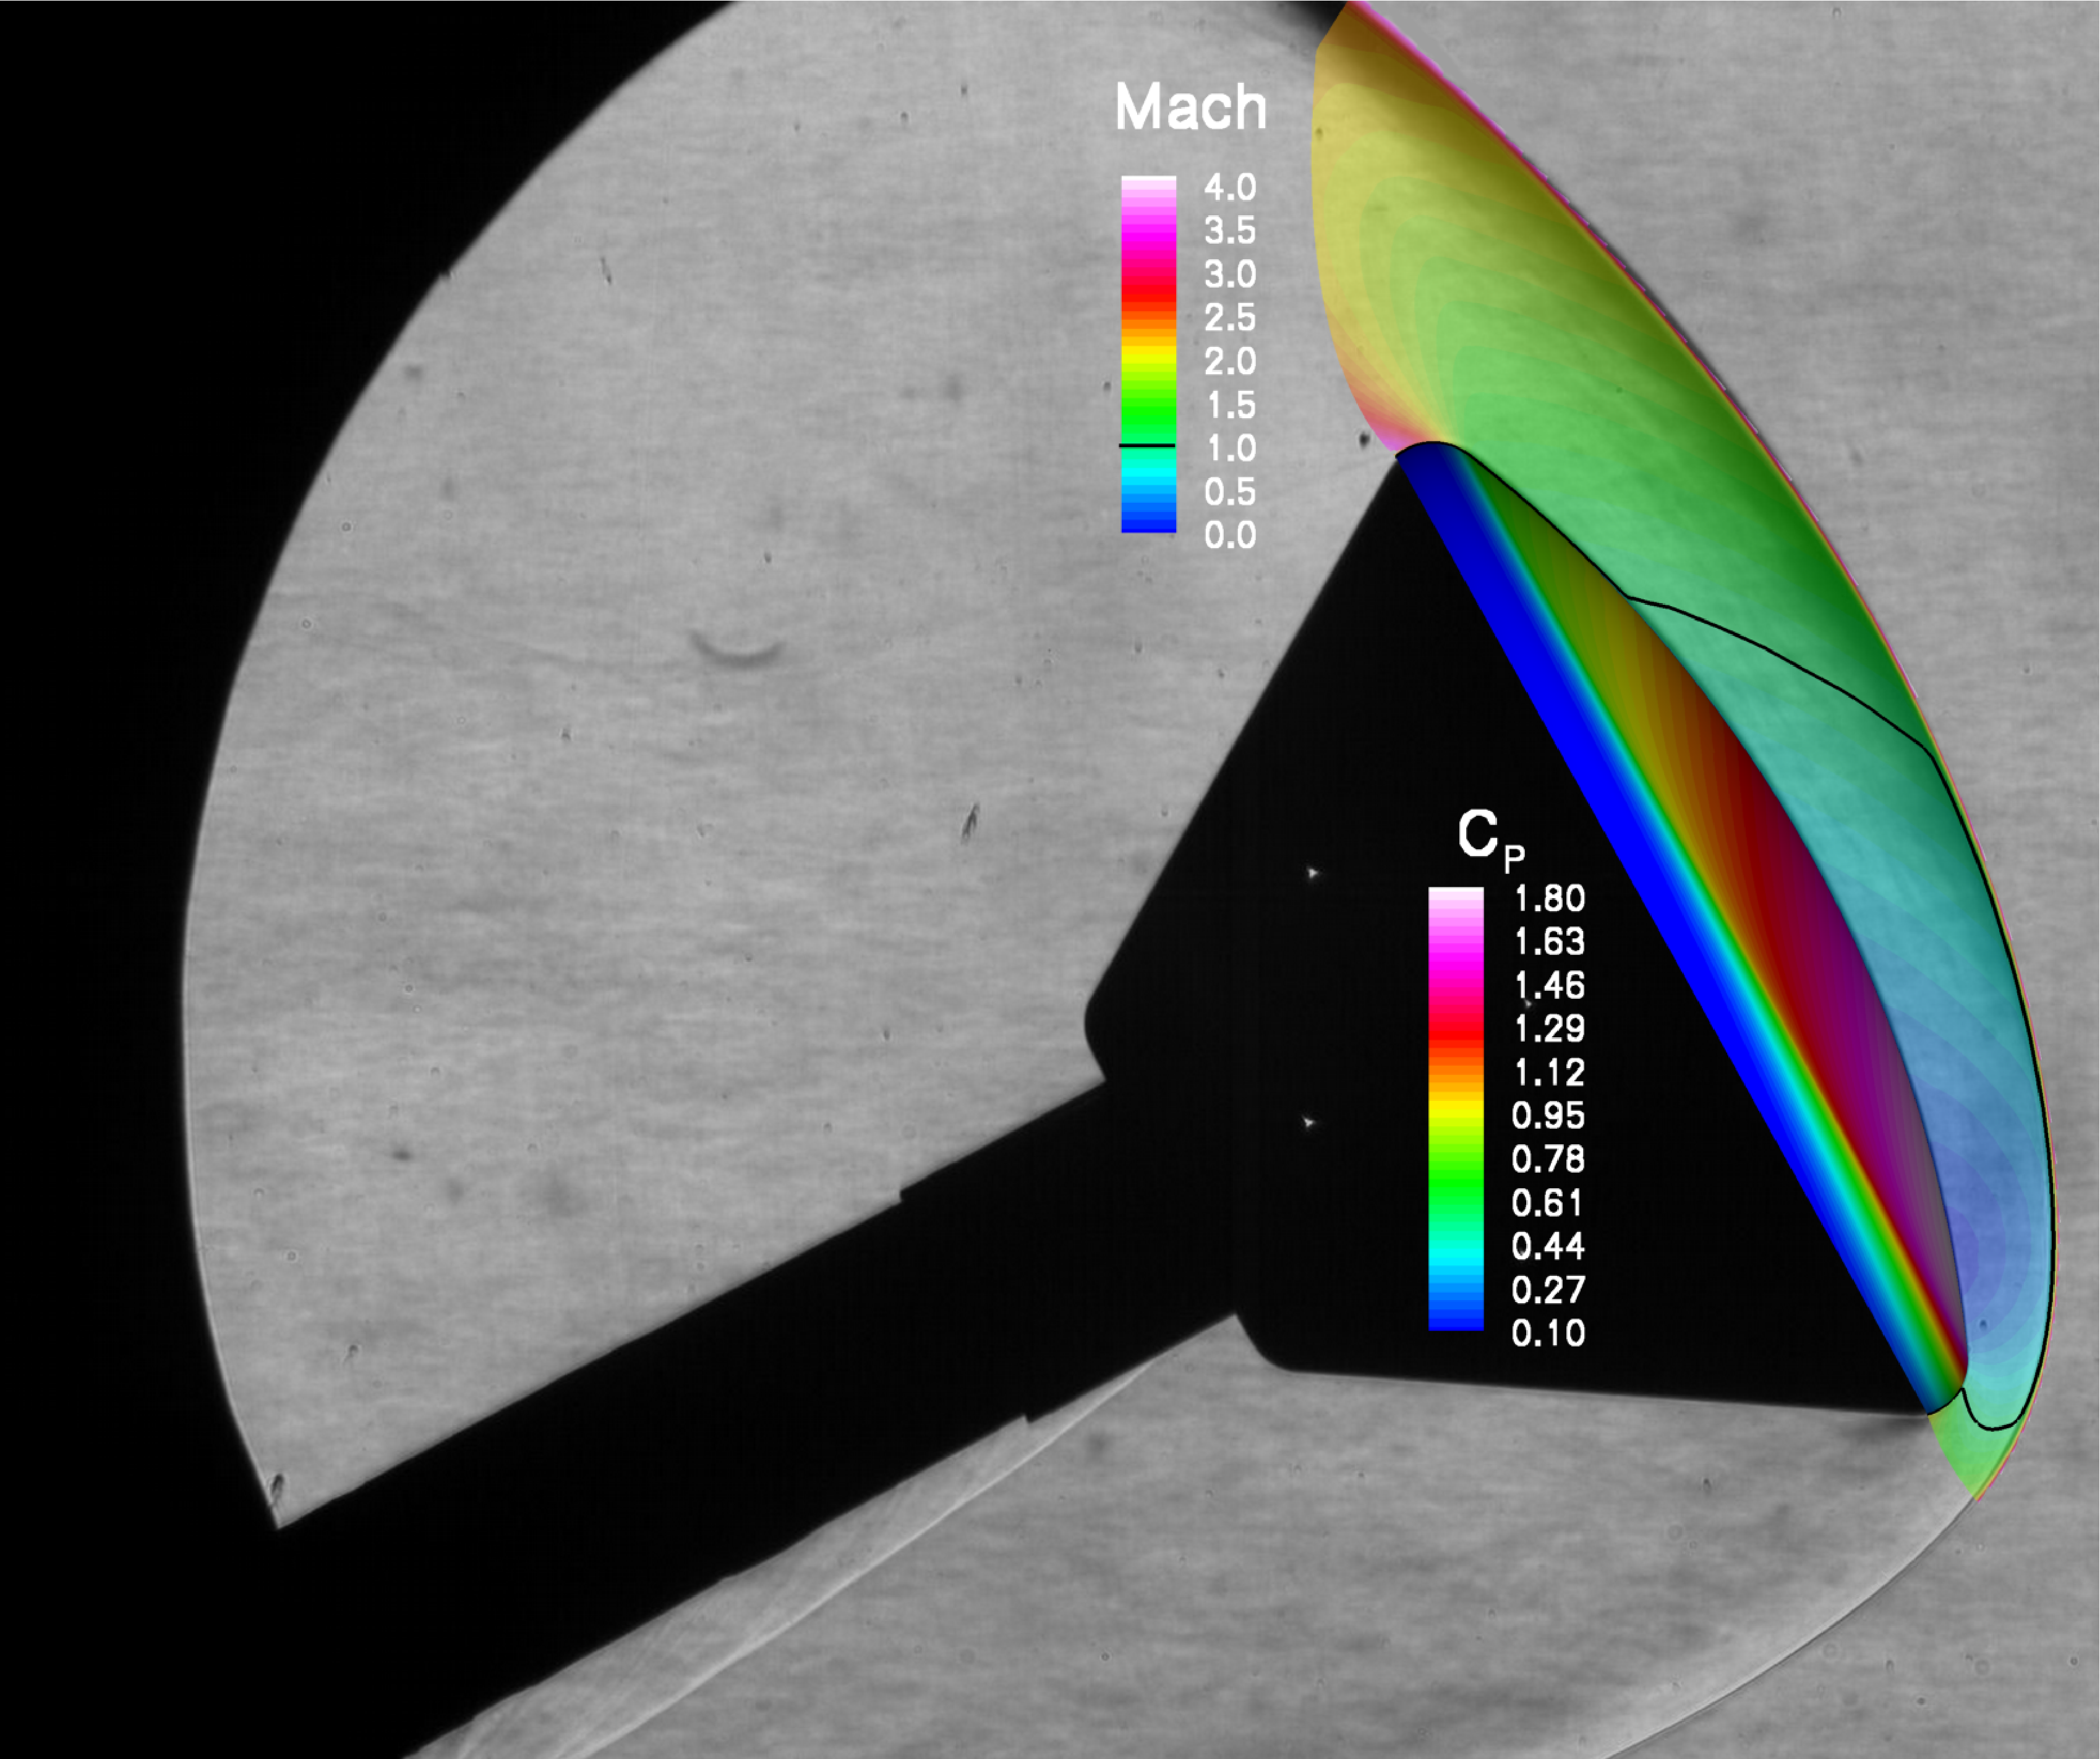
\includegraphics[width=.4\textwidth]{Benkirk_schlieren}}
        \subfigure{\label{fig:fob_redist_adapt_10_sol}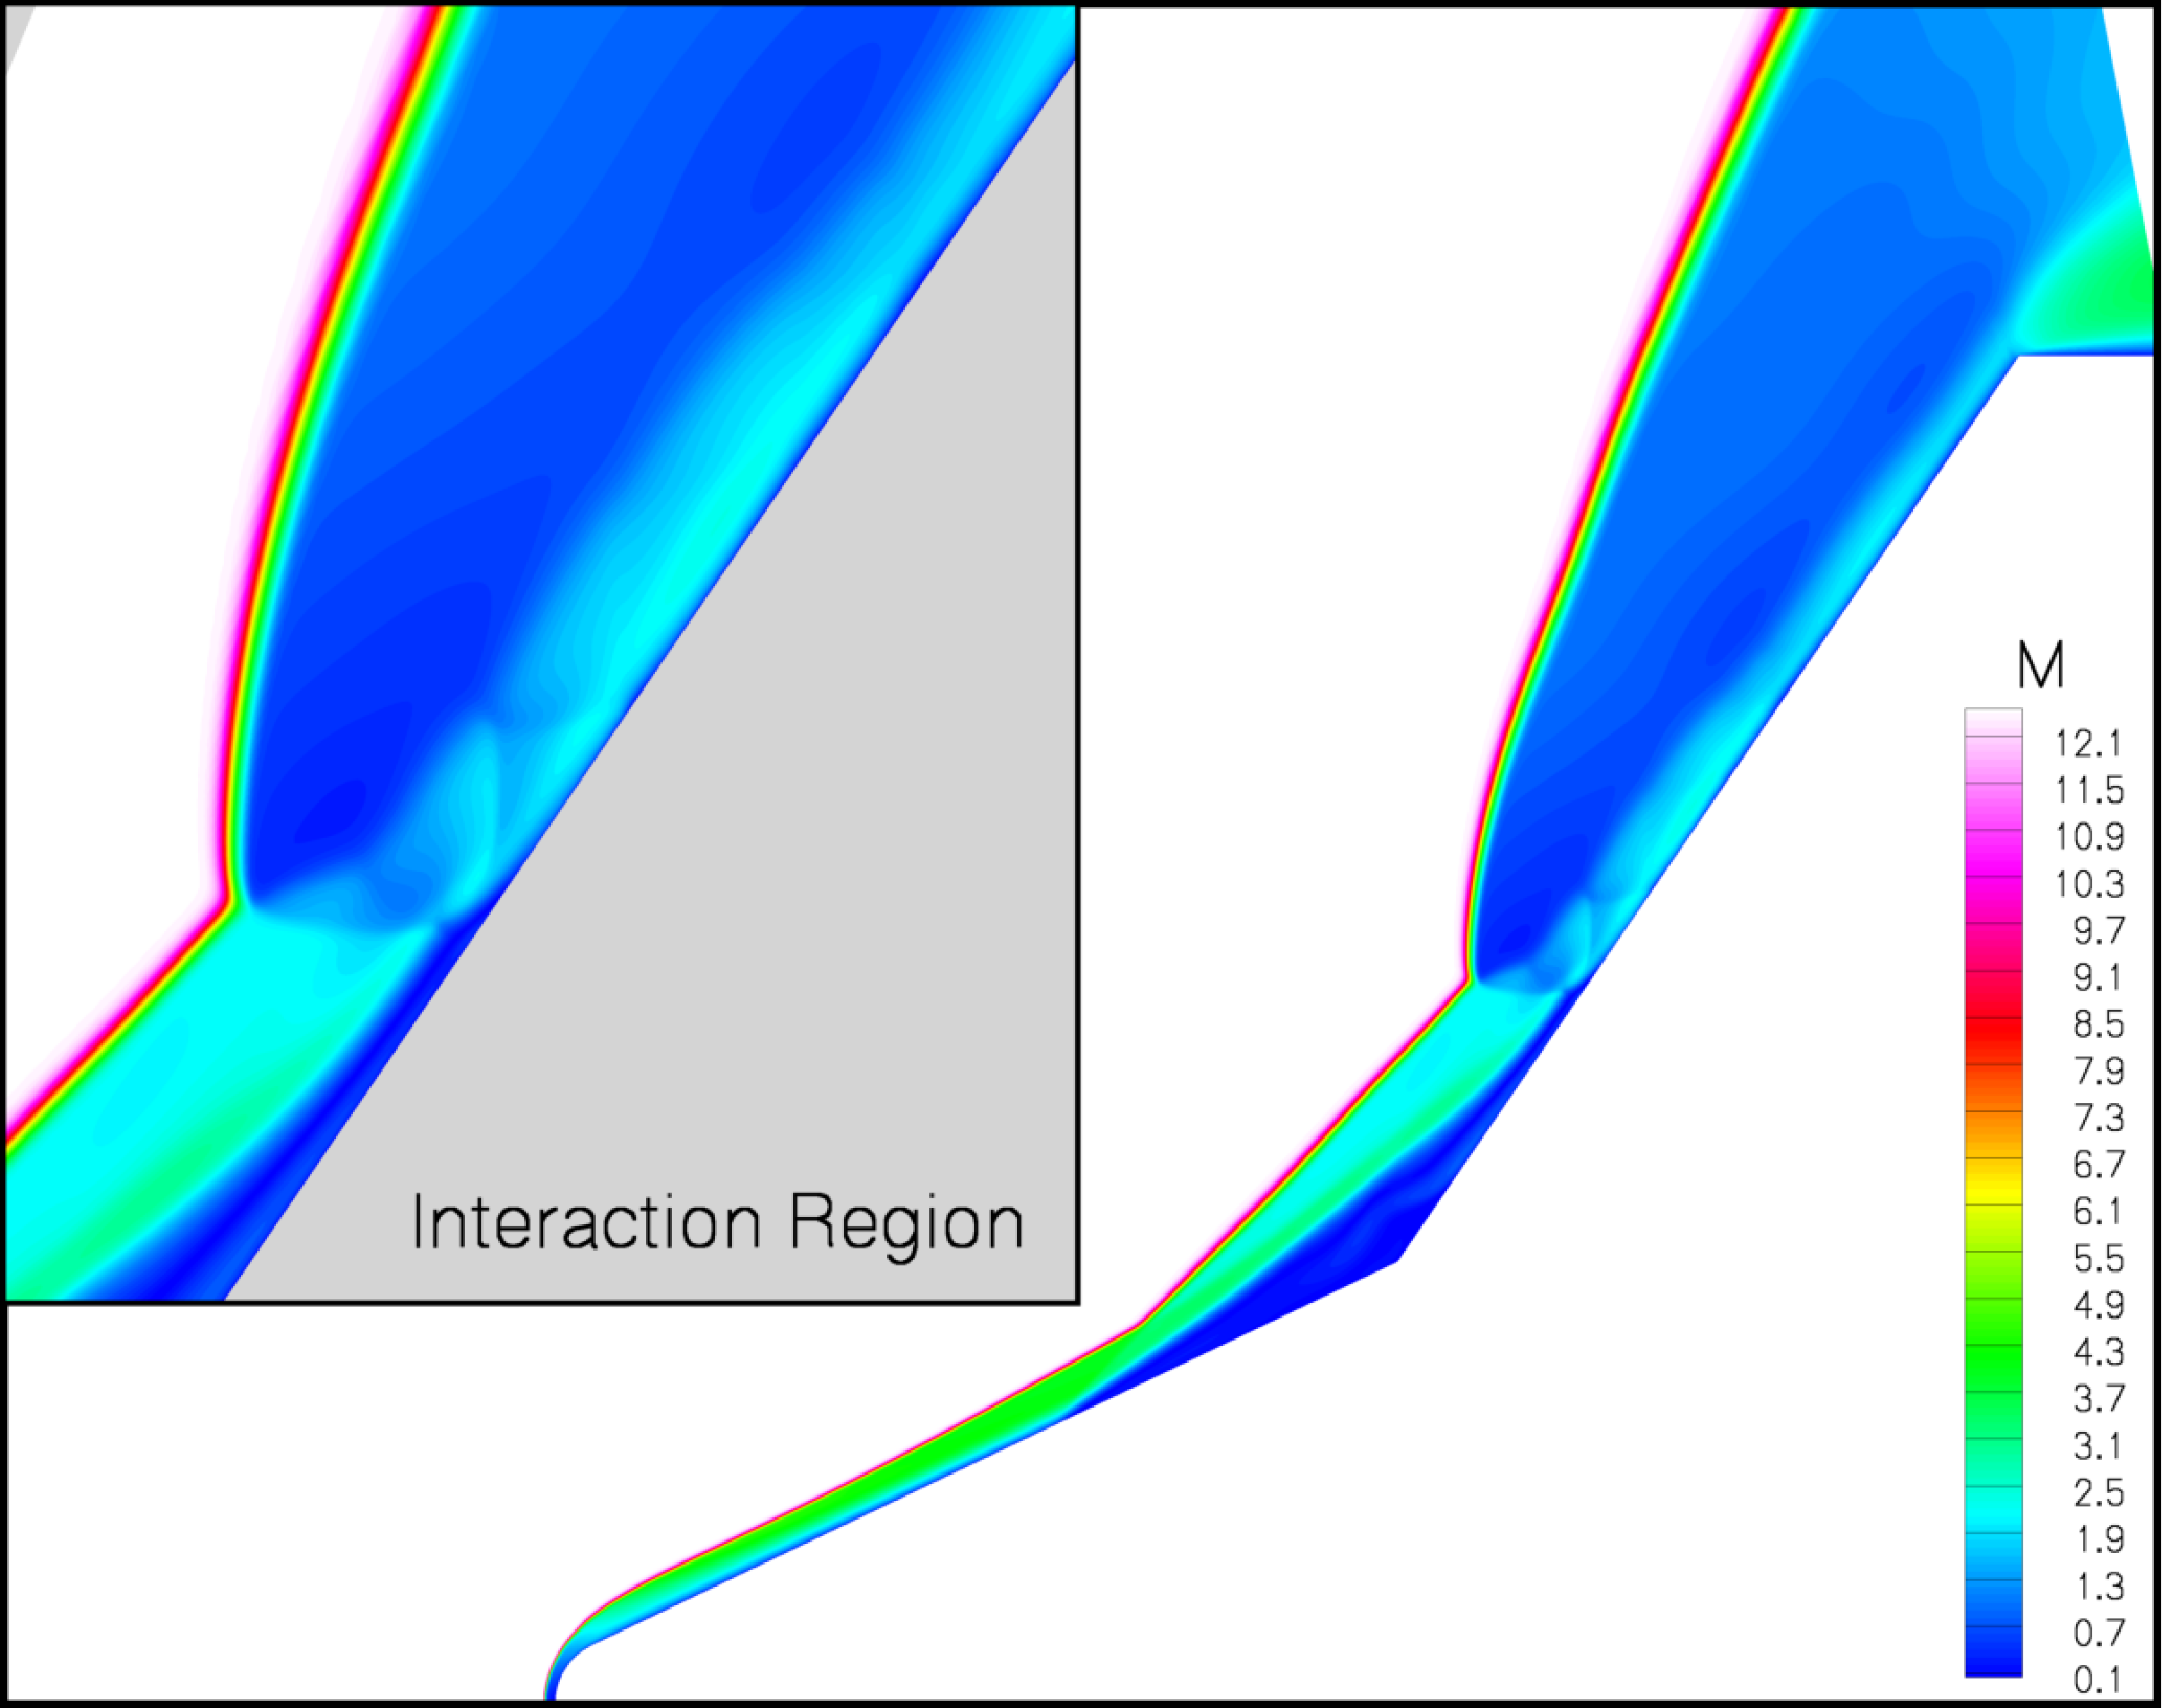
\includegraphics[width=.4\textwidth]{Benkirk_double_cone_M}}
      \end{center}
    \end{figure}
}

\section{Application Results}



%%%%%%%%%%%%%%%%%%%%%%%%%%%%%%%%%%%%%%%%%%%%%%%%%
\frame
{
  \Large
  \begin{block}{}
    \center{\textbf{Eye Candy}: Results from Physics Applications built}
    \center{on top of \bf{\libmesh{}}}
  \end{block}
}



%%%%%%%%%%%%%%%%%%%%%%%%%%%%%%%%%%%%%%%%%%%%%%%%%
\frame
{
  \frametitle{Compressible Navier-Stokes}
  \begin{center}
    \only<1>{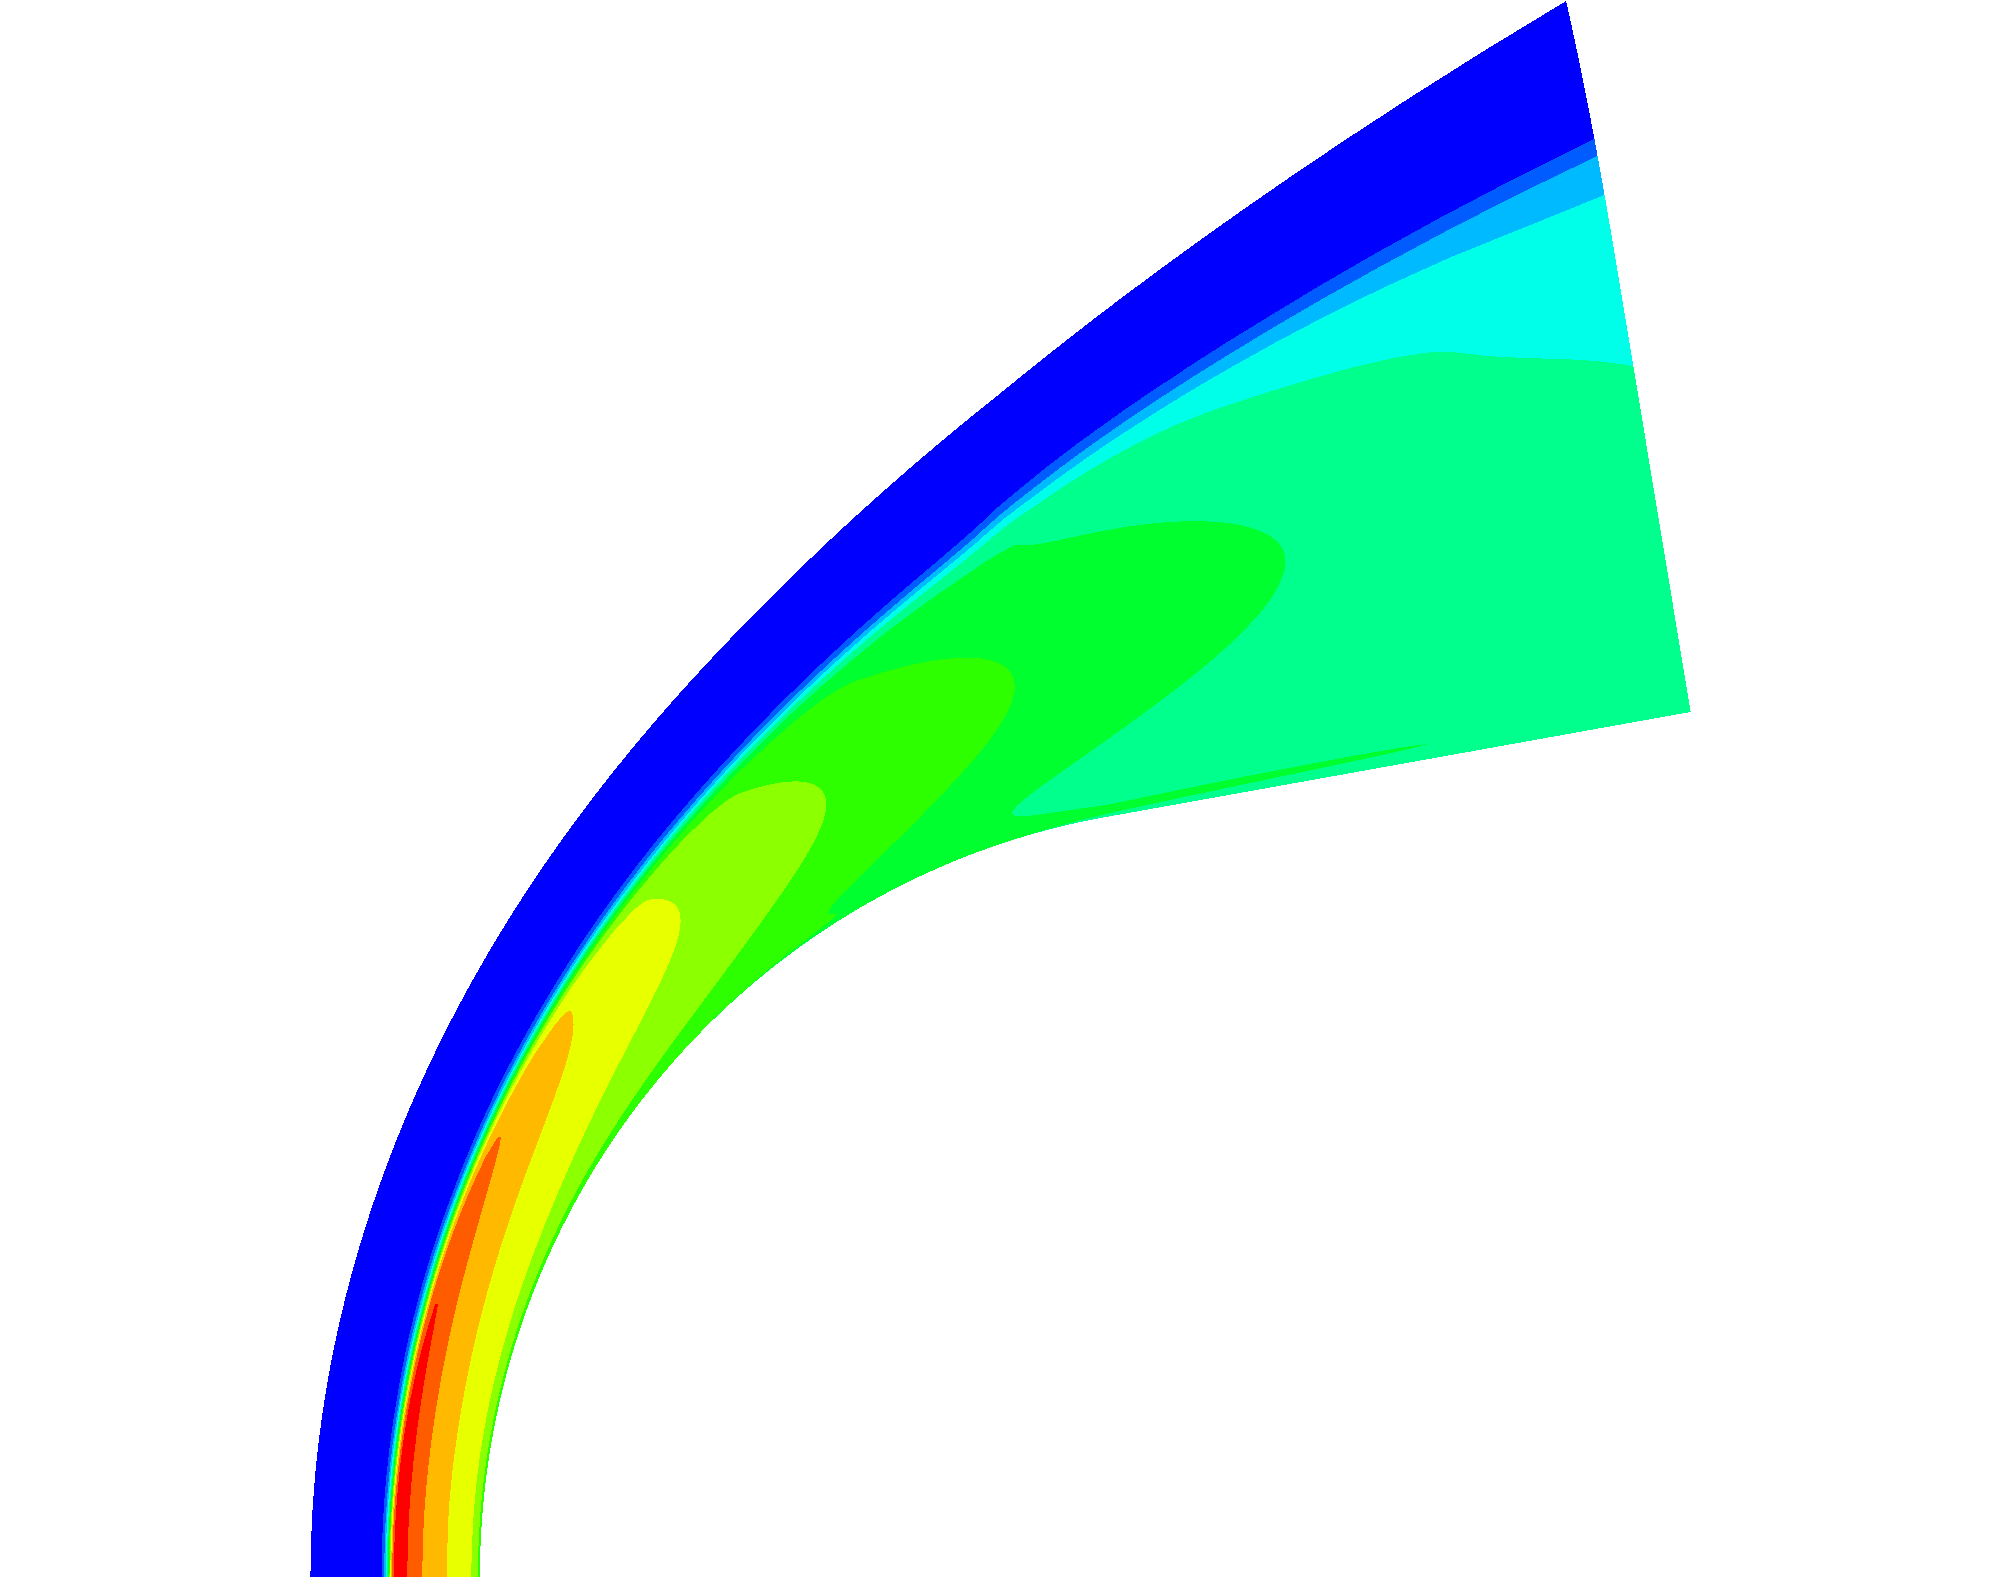
\includegraphics[height=0.9\textheight]{nosetip/smeared.png}}

    \only<2>{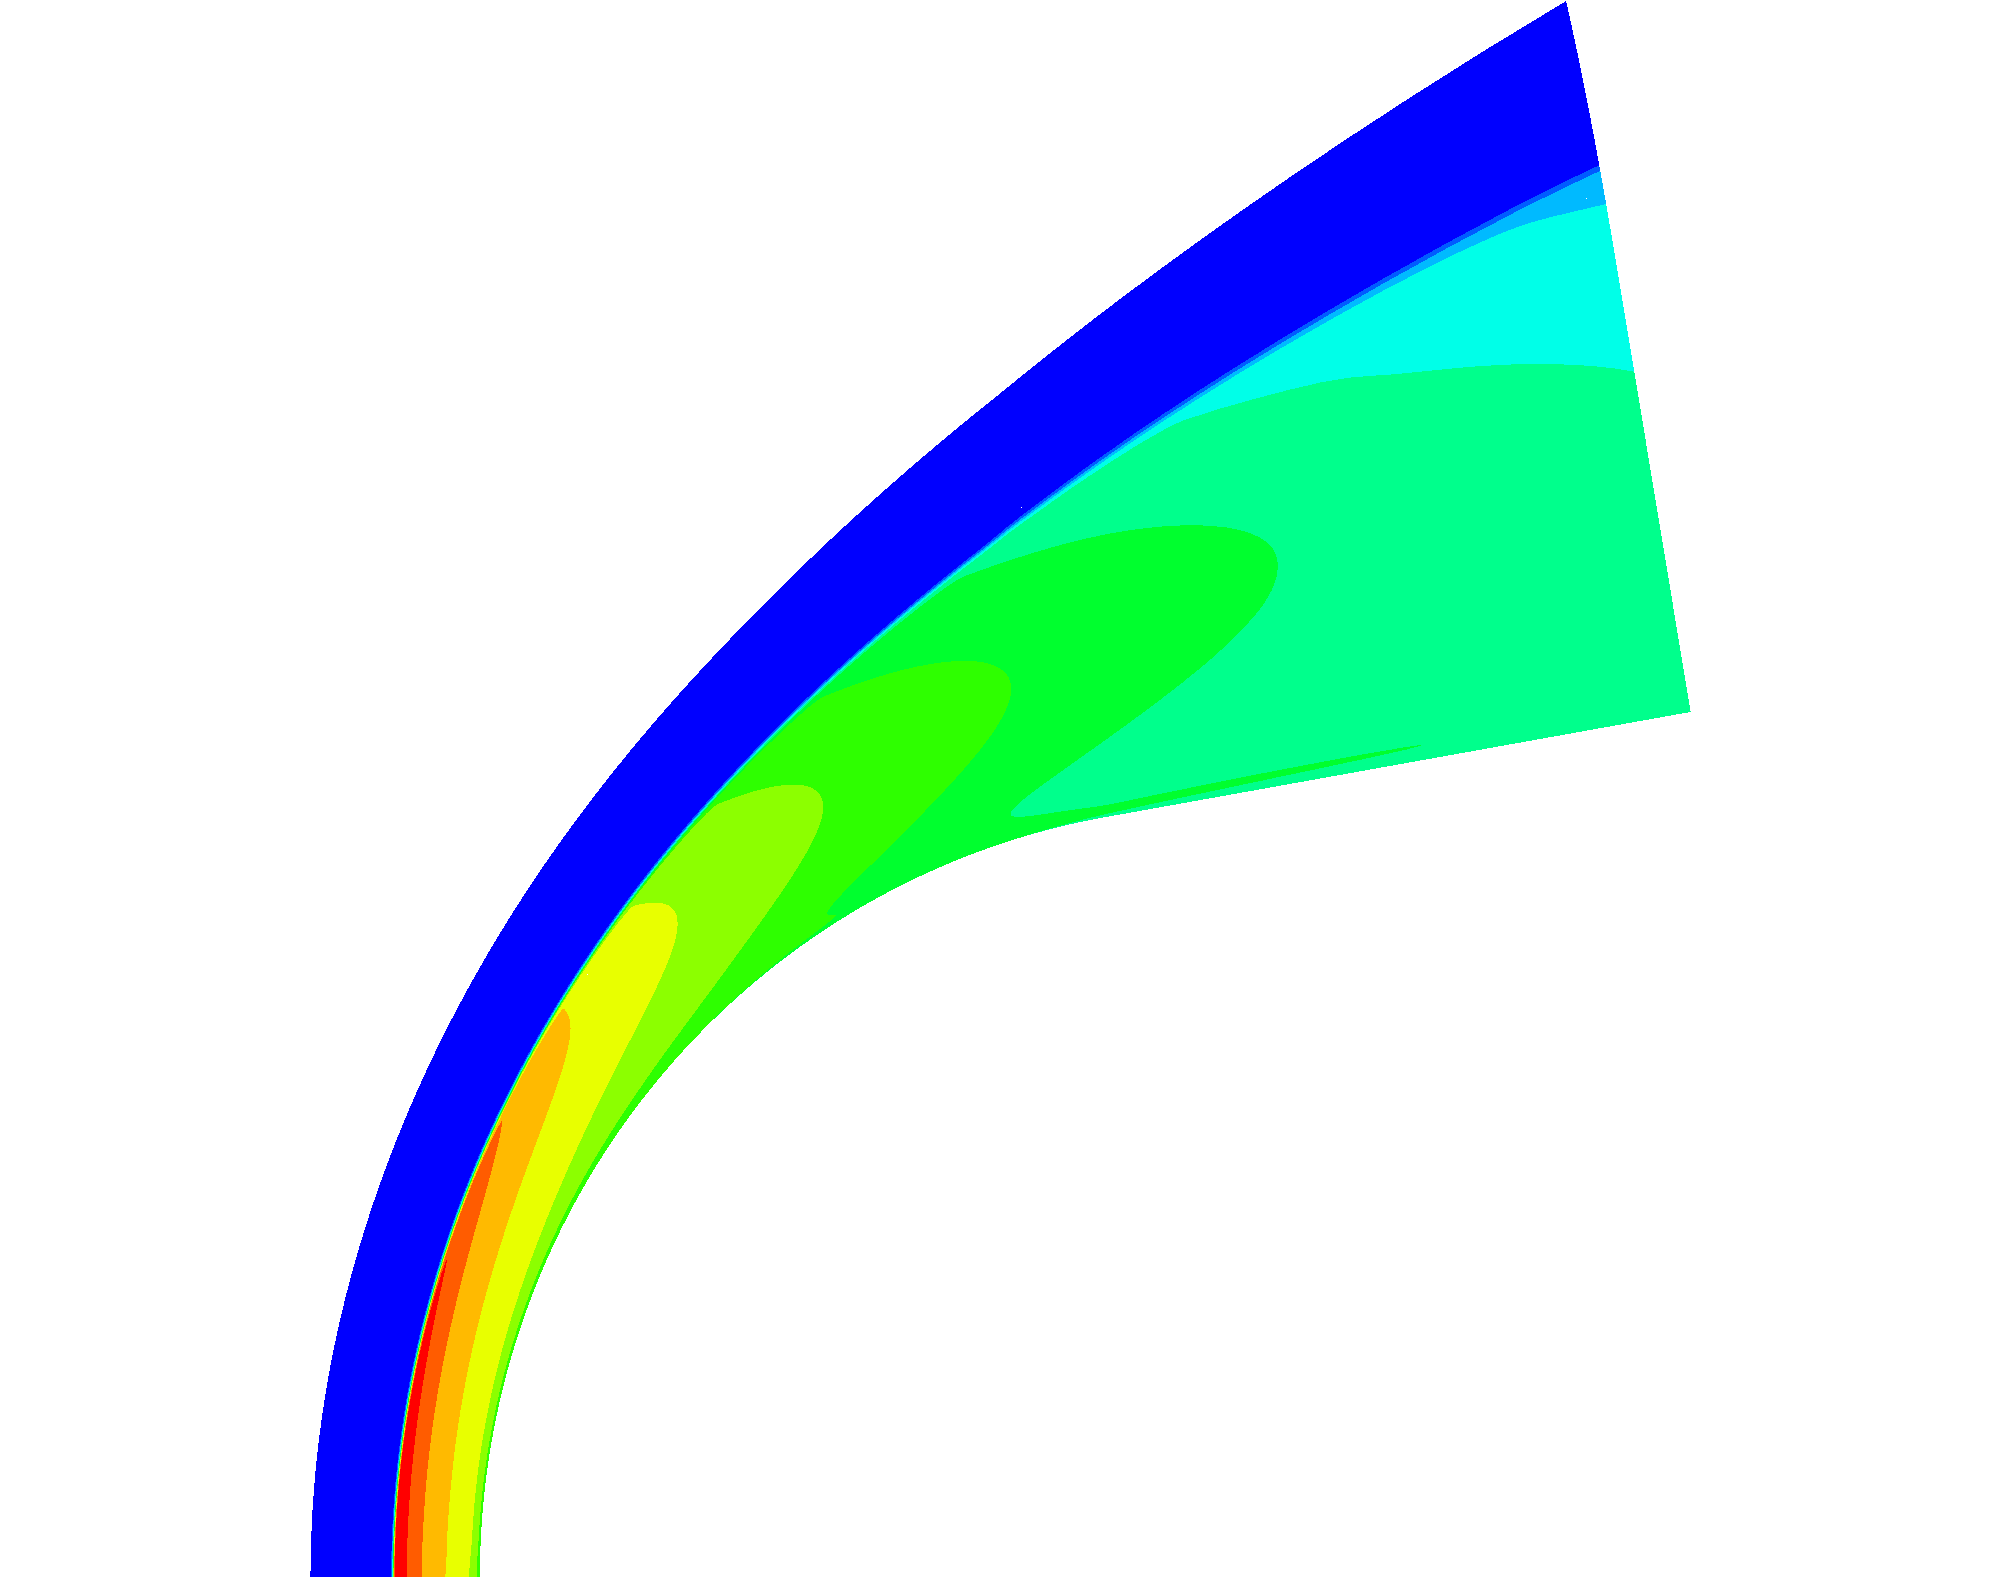
\includegraphics[height=0.9\textheight]{nosetip/amr.png}}

    \only<3>{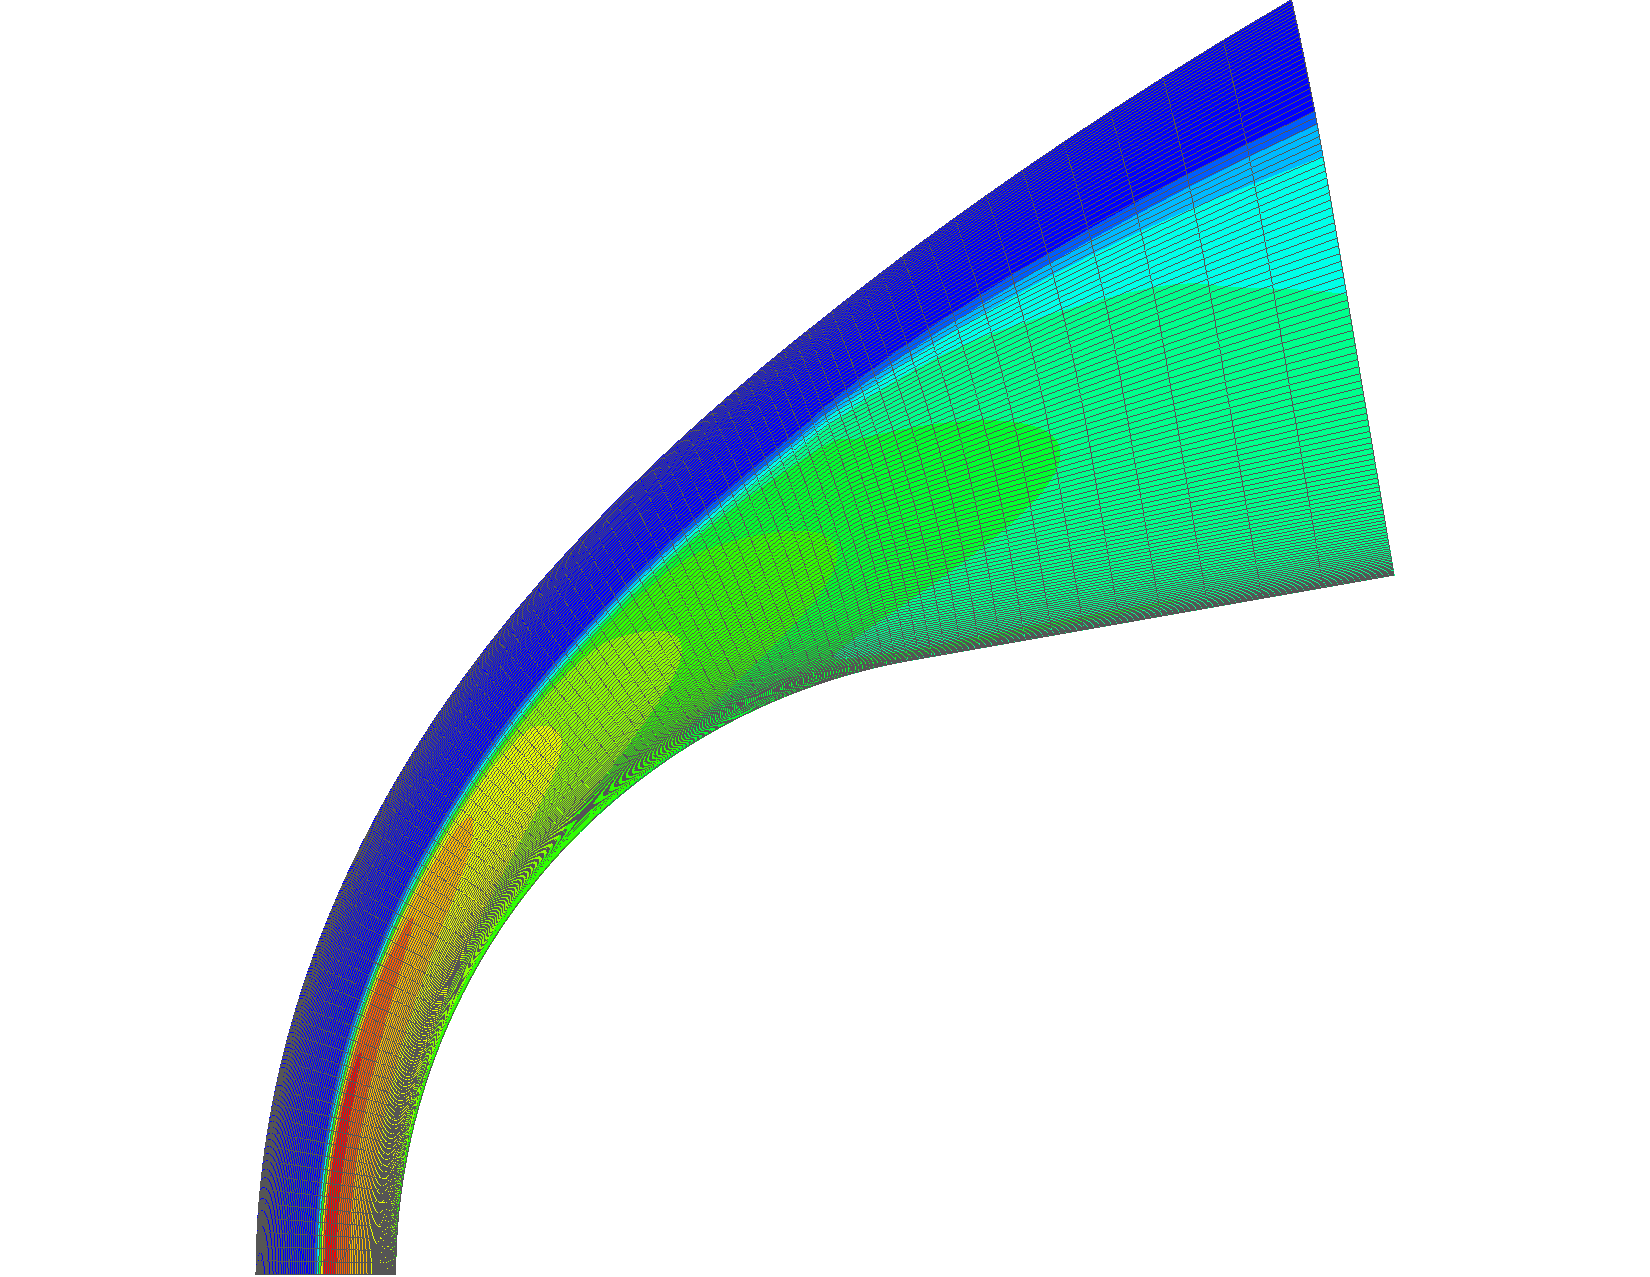
\includegraphics[height=0.9\textheight]{nosetip/smeared.pdf}}

    \only<4>{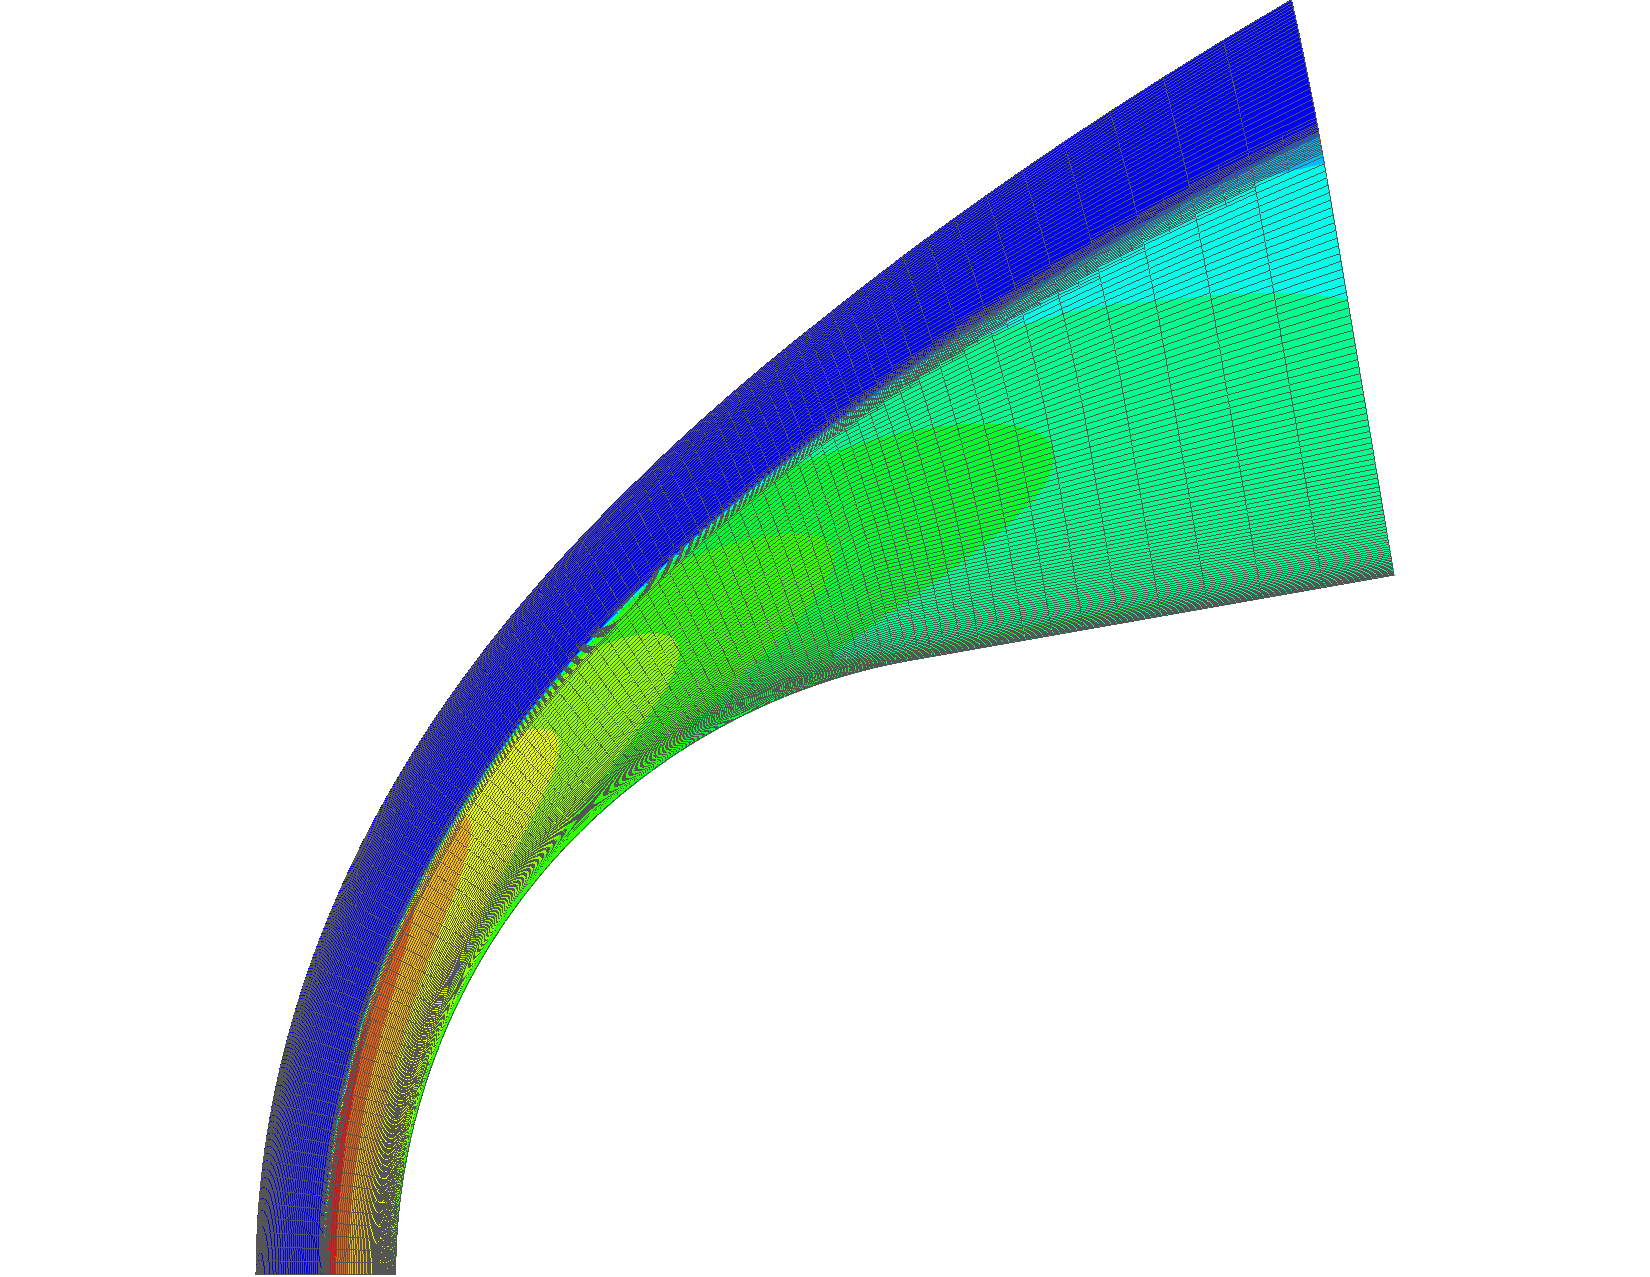
\includegraphics[height=0.9\textheight]{nosetip/amr.pdf}}

  \end{center}
}



%===============================================================================
% NEW SLIDE
%===============================================================================
\frame
{
  \frametitle{Arcjet Nozzle Calculation}
  \begin{center}

    \only<1>{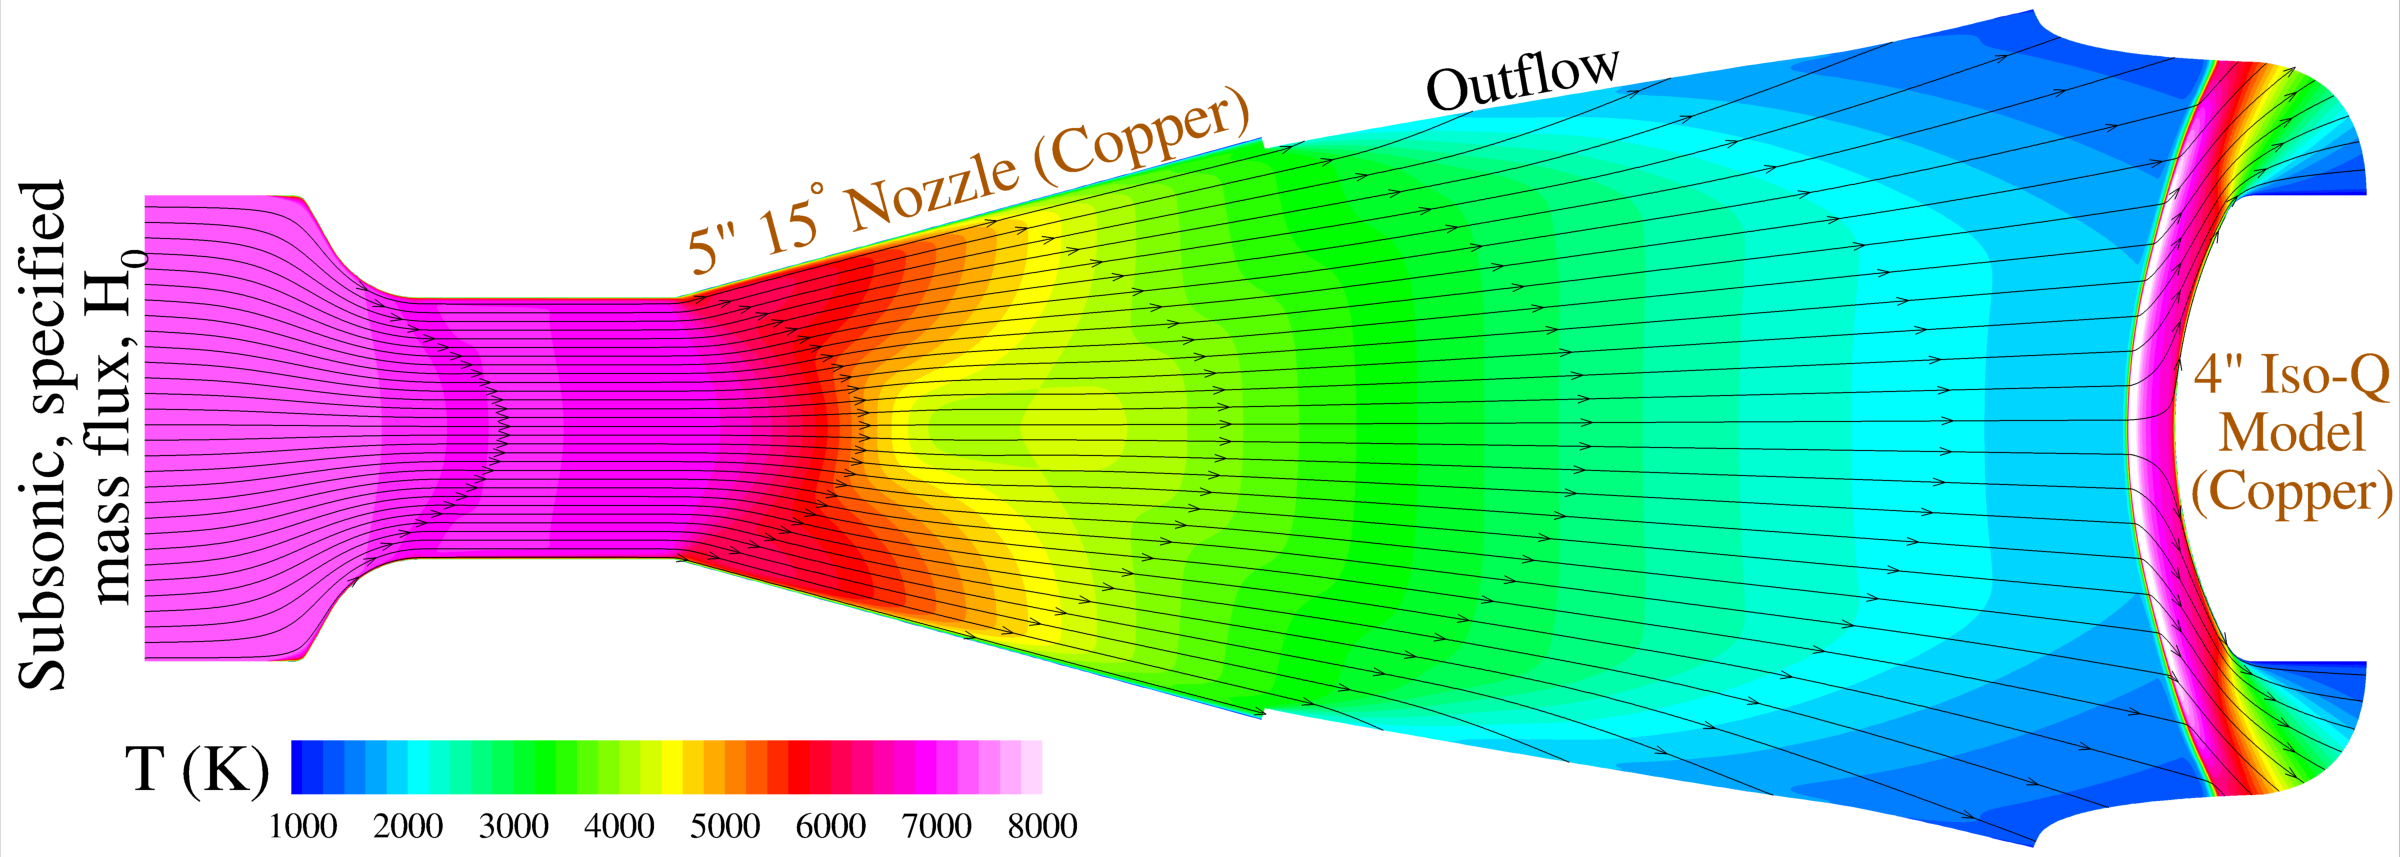
\includegraphics[width=0.95\linewidth,trim=4px 4px 4px 4px,clip]{arcjet/viz/T}}

    \only<2>{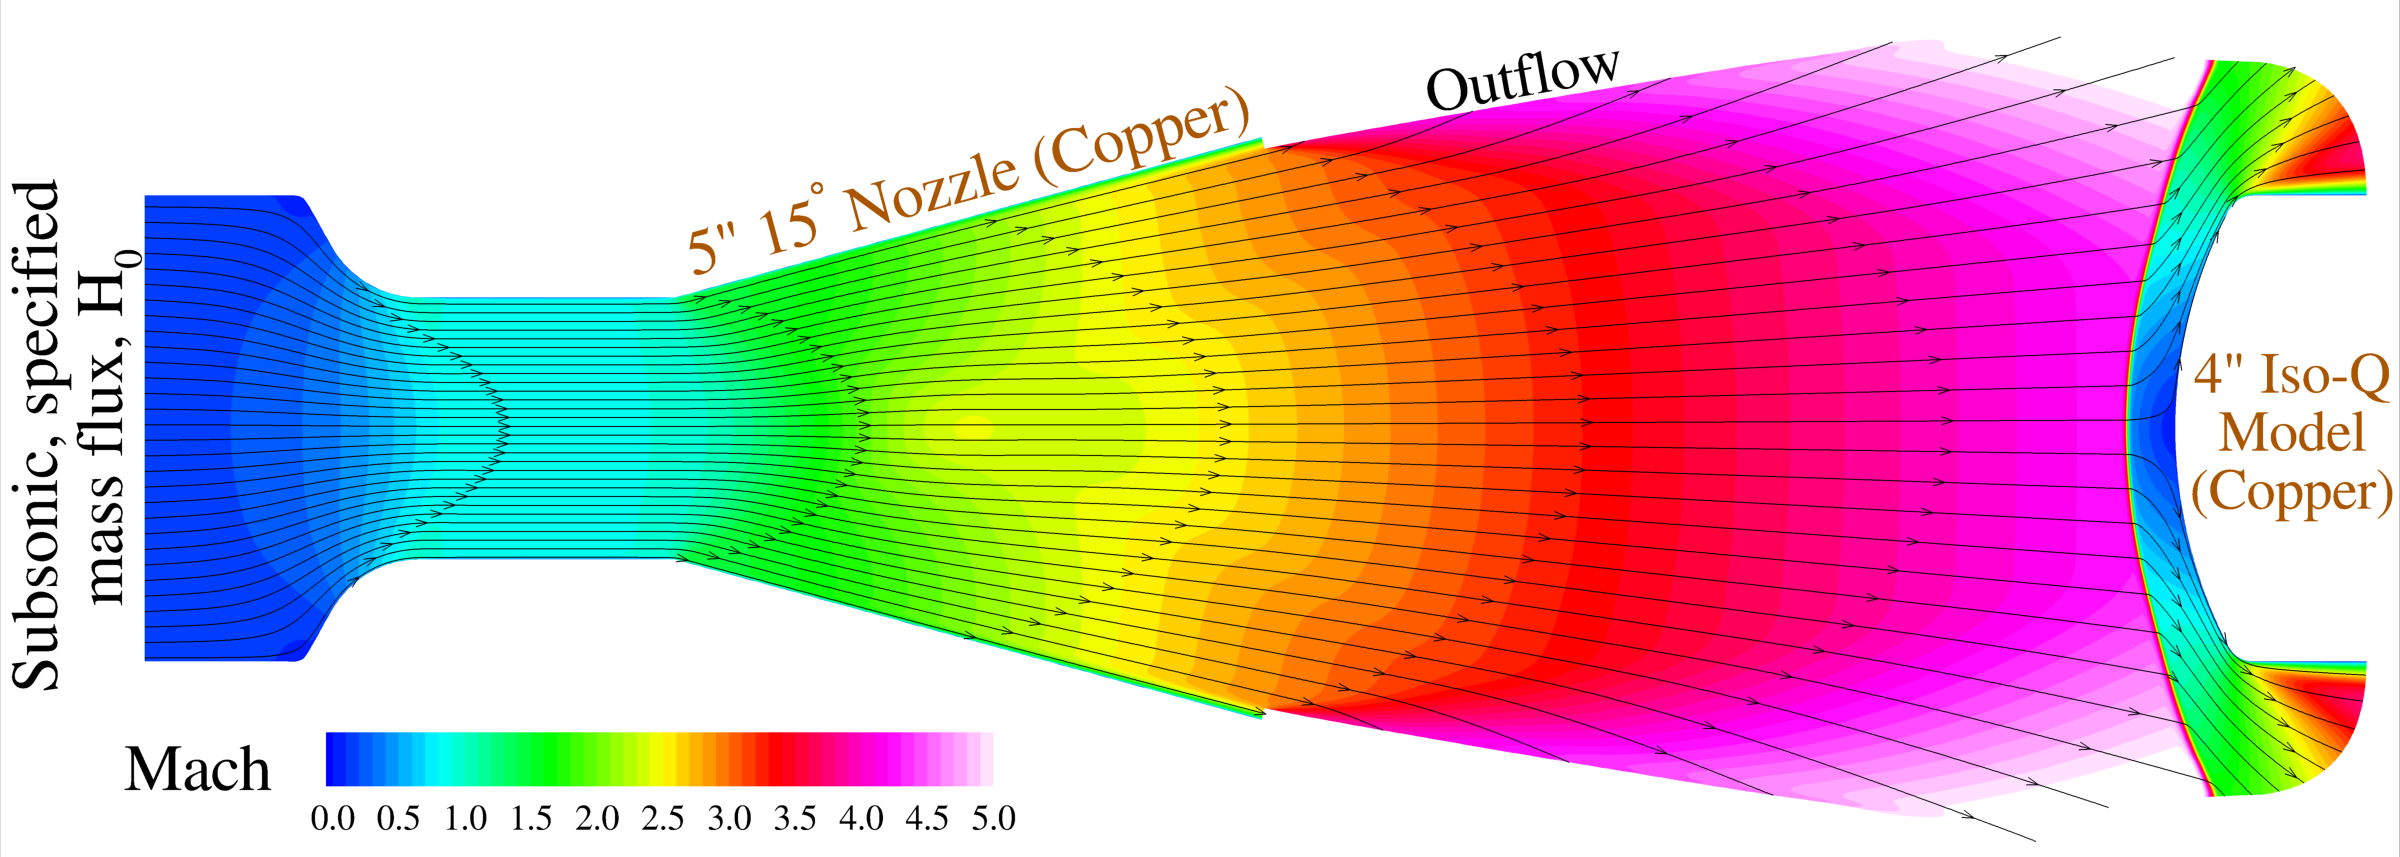
\includegraphics[width=0.95\linewidth,trim=4px 4px 4px 4px,clip]{arcjet/viz/M}}

  \end{center}
}



%===============================================================================
% NEW SLIDE
%===============================================================================
\frame
{
  \frametitle{Arcjet Nozzle Calculation}
  \begin{center}

    \only<1>{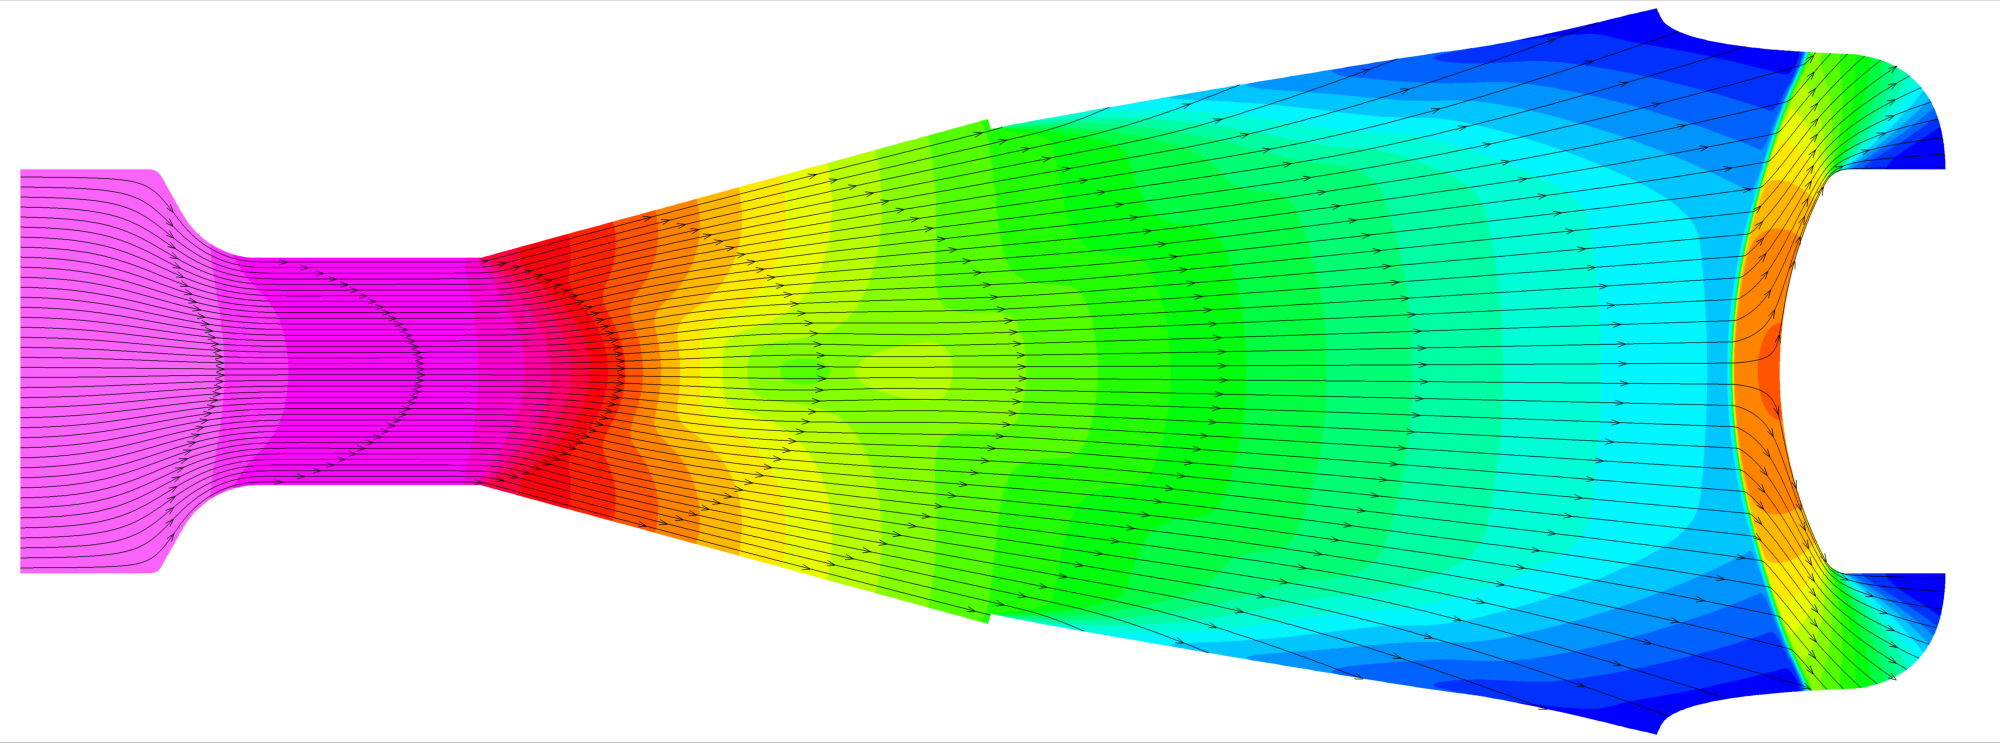
\includegraphics[width=.95\textwidth,trim=4px 4px 4px 4px,clip]{arcjet/data/nozzle/P-streamlines.png}}

    \only<2>{\includemovie[autoplay,loop,text={\includegraphics[width=.95\textwidth,trim=4px 4px 4px 4px,clip]{arcjet/data/nozzle/P-streamlines.png}}]{.95\textwidth}{}{rawfigs/arcjet/data/nozzle/P.avi}}

  \end{center}
}



%===============================================================================
% NEW SLIDE
%===============================================================================
\frame
{
  \frametitle{Coupled Pyrolysis, Temperature}
  \begin{center}

    \only<1>{\includegraphics[height=.85\textheight]{arcjet/data/coupled/T.png}}

    \only<2>{\includemovie[autoplay,loop,text={\includegraphics[height=.85\textheight]{arcjet/data/coupled/T.png}}]{}{.85\textheight}{rawfigs/arcjet/data/coupled/T.avi}}

  \end{center}
}


%% %===============================================================================
%% % NEW SLIDE
%% %===============================================================================
%% \frame
%% {
%%   \frametitle{Coupled Pyrolysis, Pyrolysis gas mass flux, $\dot{m}$}
%%   \begin{center}

%%     \only<1>{\includegraphics[height=.85\textheight]{arcjet/data/coupled/mdotzoom.png}}

%%     \only<2>{\includemovie[autoplay,loop,text={\includegraphics[height=.85\textheight]{arcjet/data/coupled/mdotzoom.png}}]{}{.85\textheight}{rawfigs/arcjet/data/coupled/mdotzoom.avi}}

%%   \end{center}
%% }



%% \frame
%% {
%%   \frametitle{Coupled Thermal/Solid Mechanics}
%%   \begin{center}

%%     \only<1>{\includegraphics[height=.85\textheight]{Gaston/pgc.png}}

%%     \only<2>{\includemovie[autoplay,loop,text={\includegraphics[height=.85\textheight]{Gaston/pgc.png}}]{}{.85\textheight}{Gaston/pgc.avi}}

%%   \end{center}
%% }



\frame
{
  \frametitle{The MOOSE Framework - Gaston et al., INL}
  \begin{center}
    \fbox{\includegraphics[page=1,height=0.8\textheight]{Gaston/talk}}
  \end{center}
}



%% \frame
%% {
%%   \frametitle{The MOOSE Framework - Gaston et al., INL}
%%   \begin{center}
%%     \fbox{\includegraphics[page=2,height=0.8\textheight]{Gaston/talk}}
%%   \end{center}
%% }



\frame
{
  \frametitle{The MOOSE Framework - Gaston et al., INL}
  \begin{center}
    \fbox{\includegraphics[page=4,height=0.8\textheight]{Gaston/talk}}
  \end{center}
}



%% \frame
%% {
%%   \frametitle{The MOOSE Framework - Gaston et al., INL}
%%   \begin{center}
%%     \fbox{\includegraphics[page=22,height=0.8\textheight]{Gaston/talk}}
%%   \end{center}
%% }

\section{Approach to Software Development}
%%%%%%%%%%%%%%%%%%%%%%%%%%%%%%%%%%%%%%%%%%%%%%%%%
\frame
{
  \Large
  \begin{block}{}
    \center{\bf Sidebar: Important websites}
    \begin{itemize}
      \item \href{http://libmesh.sourceforge.net}{Primary website}
      \item \href{http://github.com/libMesh/libmesh}{Revision Control \& Collaboration with GitHub}
      \item \href{http://buildbot.ices.utexas.edu:8010/waterfall}{Continuous Integration with Buildbot}
        %% \begin{itemize}
        %%   \item \href{http://buildbot.ices.utexas.edu:8010/builders/libmesh\%2Fmaster}{Vanilla Master}
        %%   \item \href{http://buildbot.ices.utexas.edu:8010/builders/libmesh\%2Fmaster%2Bsl6options}{Options}
        %% \end{itemize}
    \end{itemize}
  \end{block}
}


\frame
{
\frametitle{\url{http://libmesh.sourceforge.net}}

\centerline{\includegraphics[width=0.85\textwidth]{trivia/libmesh_site}}
}


\frame
{
\frametitle{\url{http://github.com/libMesh/libmesh}}

\centerline{\includegraphics[width=0.85\textwidth]{trivia/github_site}}
}


\frame
{
\frametitle{\scriptsize \url{http://buildbot.ices.utexas.edu:8010/waterfall}}

\centerline{\includegraphics[width=0.85\textwidth]{trivia/buildbot_site}}
}


\begin{frame}[fragile]
  \frametitle{Getting the \libMesh{} Source}

  \begin{block}{}
    \begin{itemize}
    \item \textbf{Blessed, Stable releases:}

      Download prepackaged releases from

      \scriptsize{\url{http://sourceforge.net/projects/libmesh/files/libmesh}}
      \normalsize
    \item \textbf{Development tree:}

      Grab the latest source tree from GitHub:
      \begin{lstlisting}[language=bash]
        git clone git://github.com/libMesh/libmesh.git
      \end{lstlisting}
    \end{itemize}
  \end{block}
\end{frame}


\begin{frame}[fragile]
  \frametitle{Building \libMesh{} from source}

  \begin{block}{Unpack, Configure, Build, Install, \& Test}
    \begin{lstlisting}[language=bash]
      tar jxf libmesh-0.9.1.tar.bz2 && cd libmesh-0.9.1
      ./configure --prefix=`pwd`/install
      make -j 4 && make -j 4 install && make -j 4 check METHODS=opt
      make -j 4 installcheck
    \end{lstlisting}
\end{block}
\end{frame}

\section{A Generic Boundary Value Problem}
%%%%%%%%%%%%%%%%%%%%%%%%%%%%%%%%%%%%%%%%%%%%%%%%%
\frame
{
  \Large
  \begin{block}{}
    \center{Solving Problems the {\bf \libmesh{}} way}
    \center{Discretizing a Generic Boundary Value Problem}
  \end{block}
}



\subsection*{What class of problems is LibMesh designed to solve?}
% The ``Generic BVP'' slide has been slightly revamped for notational consistency
\begin{frame}[t]
  %\frametitle{A Generic BVP}
  \begin{columns}[t]
    \column{.5\textwidth}
     \begin{itemize}
      \item General boundary value problems of the form:
      \end{itemize}
%    \begin{block}{}%{We assume there is a Boundary Value Problem of the form}
      \vspace{-.1in}
        \begin{eqnarray}
	\label{eqn:general_pde}
	\nonumber
	M \frac{\partial u}{\partial t} & = & F( u ) \;\;\;\; \in \Omega
        \\
	\nonumber
	G( u ) & = & 0 \;\;\;\;\;\;\;\;\; \in \Omega
	\\
	\nonumber
	u & = & u_D \;\;\;\;\;\;\; \in \partial \Omega_D
	\\
	\nonumber
	N(u) & = & 0 \;\;\;\;\;\;\;\;\; \in \partial \Omega_N
 	\\
 	\nonumber
 	u(\bv{x}, 0) & = & u_0(\bv{x}) 
      \end{eqnarray}
%    \end{block}
    %\pause
    \column{.5\textwidth}
      \begin{center}
	\includegraphics[viewport=140 420 400 685,clip=true,width=2in]{figures/domain2/domain2_input}
      \end{center}
  \end{columns}
\end{frame}

\begin{frame}
  %\frametitle{}
  \begin{columns}[t]
    \column{.5\textwidth}
    \begin{block}{}%A general class of PDE}
      \begin{itemize}
      \item{
	Associated to the problem domain $\Omega$ is a LibMesh data
	structure called a \texttt{Mesh}
      }
	
      \item{A \texttt{Mesh} is essentially
	a collection of finite elements}
      \end{itemize}
      \begin{equation}
	\label{eqn:discretized_domain}
	\nonumber
	\Omega^h:=\bigcup_e \Omega_e
      \end{equation}
    \end{block}
    %\pause
    \column{.5\textwidth}
    %\begin{block}{}
      \begin{center}
	%\fbox{
	\includegraphics[width=2in,angle=-90]{discretized_domain}
	%}
      \end{center}
    %\end{block}
  \end{columns}
  \visible<2>
  {
  \begin{itemize}
    \item{LibMesh provides some simple structured mesh generation
routines, file inputs, and interfaces to Triangle and TetGen.}
  \end{itemize}
  }
\end{frame}


\begin{frame}[shrink]
  \frametitle{The Mesh}
  
  \lstinputlisting[language=C++]{snippets/mesh.cxx}

\end{frame}


\section{Key Data Structures}

%%%%%%%%%%%%%%%%%%%%%%%%%%%%%%%%%%%%%
\subsection{The Mesh Class}
\begin{frame}[shrink]
  \frametitle{The Mesh}  
  \lstinputlisting{snippets/mesh.cxx}
\end{frame}


\begin{frame}[shrink]
  \frametitle{The Mesh}  
  \lstinputlisting[language=bash]{snippets/mesh.cxx.out}
\end{frame}

%%%%%%%%%%%%%%%%%%%%%%%%%%%%%%%%%%%%%
\subsection{The EquationSystems Class}
\begin{frame}[shrink]
  %\frametitle{EquationSystems}  
  \lstinputlisting{snippets/es.cxx}
\end{frame}

\section{Weighted Residuals}
% Auto-generate the TOC slide(s)
\begin{frame}
  \tableofcontents[currentsection]
  %\tableofcontents
\end{frame}


\begin{frame}[<+->]
      %\frametitle{Weighted Residual Statement}
  \begin{itemize}
  \item {The point of departure in any FE analysis which uses \libMesh{} is
    the weighted residual statement
    %(sometimes referred to as simply ``the residual'' in
    %the documentation.)
    \begin{equation}
      \nonumber
      (F( u ), v) = 0 \hspace{.5in} \forall v \in \mathcal{V}
    \end{equation}
    }

  \item{ Or, more precisely, the weighted residual statement associated with the
    finite-dimensional space $\mathcal{V}^h \subset \mathcal{V}$
    \begin{equation}
      \nonumber
      (F( u^{\alert{h}} ), v^{\alert{h}}) = 0 \hspace{.5in} \forall v^{\alert{h}} \in \mathcal{V}^{\alert{h}}
  \end{equation}}

  \end{itemize}
\end{frame}


\subsection*{Some Examples}    
\begin{frame}[t]
  %\frametitle{Some Examples}
    \begin{block}{
	\only<1-2>{Poisson Equation}
	\only<3-4>{Linear Convection-Diffusion}
	\only<5-6>{Stokes Flow}
      }

      \only<1-2>
      {
	\begin{equation}
	      \nonumber
	      -\Delta u  = f
	      \hspace{.25in} \in \hspace{.1in} \Omega  
	    \end{equation}
      }
      
      \only<3-4>
	  {
	    \begin{equation}
	      \nonumber
	      %\frac{\partial u}{\partial t}
	      -k\Delta u + \bv{b} \cdot \nabla u = f
	      \hspace{.25in} \in \hspace{.1in} \Omega  
	    \end{equation}
	  }

      \only<5-6>
      {
	\begin{equation}
	    \begin{array}{rcl}
	      \nonumber
	      %\frac{\partial \bv{u}}{\partial t} +
	      %\left(\bv{u} \cdot \nabla\right) \bv{u} +
	      \nabla p - \nu \Delta \bv{u}  &=& \bv{f}
	        \\
	      \nonumber
	      \nabla \cdot \bv{u} &=& 0
	    \end{array}  \hspace{.25in}  \in \hspace{.1in} \Omega
	\end{equation}
      }

      
\end{block}
    %\pause

    \only<2,4,6>
    {
    \begin{block}{Weighted Residual Statement}
    }
      \only<2>
      {
      \begin{eqnarray}
	\nonumber
	(F( u ), v) := %\hspace{3in} \\  \nonumber
	\int_{\Omega}  \left[ \nabla u \cdot \nabla v - fv \right] dx \\ \nonumber
	+ \int_{\partial \Omega_N} \left(\nabla u \cdot \bv{n}\right) v \;ds
      \end{eqnarray}
%%       $^{\ast}$ We have employed the divergence theorem to obtain the weighted residual statement.
%%       In general this procedure gives rise to boundary terms which for simplicity we do not discuss
%%       in detail.
      }
      
    \only<4>
    {
      \begin{eqnarray}
	\nonumber
	(F( u ), v) := 
	\int_{\Omega} \left[
	  %\tfrac{\partial u}{\partial t}v  +
	  k\nabla u \cdot \nabla v + (\bv{b} \cdot \nabla u) v - fv \right] dx \\ \nonumber
	+ \int_{\partial \Omega_N} k\left(\nabla u \cdot \bv{n}\right) v \;ds
      \end{eqnarray}
    }

    \only<6>
    {
      \vspace{-.2in}
      \begin{eqnarray}
	\nonumber
	u := \left[\bv{u}, p\right]
	\hspace{.1in},\hspace{.1in}
	v := \left[\bv{v}, q\right]
      \end{eqnarray}
      \vspace{-.25in}
	\begin{eqnarray}
	  \nonumber
	(F( u ), v) := %\hspace{3in} \\ \nonumber
	\int_{\Omega} \left[
	  %\left( \tfrac{\partial \bv{u}}{\partial t}	  +
	  %\left( \bv{u} \cdot \nabla  \right)\bv{u}
	  %\right)
	  %\cdot \bv{v}
	- p\left(\nabla \cdot \bv{v}\right) 
	+ \nu \nabla \bv{u} \colon\!\! \nabla \bv{v} - \bv{f}\cdot \bv{v} \; \right. \\ \nonumber
	+ \left.\left( \nabla \cdot \bv{u} \right) q \right] dx
	+ \int_{\partial \Omega_N} \!\!\bv{n} \cdot \left(\nu \nabla \bv{u} -p\bv{I}\right) \cdot \bv{v} \;ds %\hspace{1in}	
      \end{eqnarray}
    }
\only<2,4,6>
{
    \end{block}
 }     
\end{frame} 



%\subsection*{Approximate Problem}
\begin{frame}%[<+->]
  %\frametitle{Weighted Residual Statement}
  \begin{itemize}

    %%   \item{In each of the examples, the weighted residual statement is obtained by
    %%     multiplying the PDE by a test function $v$, integrating over the domain $\Omega$,
    %%     and applying the divergence theorem.}

    %%   \item{Since $v=0$ on $\partial \Omega_D$ (essential data) the boundary integrals
    %%     are over $\partial \Omega_N$ only.}

    %%   \item{There are simple and efficient techniques (e.g.\ penalty method) for
    %%     enforcing the Dirichlet conditions.}

  \item{To obtain the approximate problem, we simply
    replace $u \leftarrow u^h$, $v \leftarrow v^h$, and $\Omega \leftarrow \Omega^h$
    in the weighted residual
    statement.}
    
  \end{itemize}
\end{frame}

\section{Poisson Equation}
% Auto-generate the TOC slide(s)
\begin{frame}
  \tableofcontents[currentsection]
  %\tableofcontents
\end{frame}


\subsection*{Weighted Residual Statement}
\begin{frame}%[<+->]
  %\frametitle{Poisson Equation}
  \begin{itemize}
  \item {For simplicity we start with the weighted
    residual statement arising from the Poisson equation,
    with $\partial \Omega_N = \emptyset$, 
    \begin{eqnarray}
      \nonumber
      (F( u^h ), v^h) := \hspace{2.5in} \\  \nonumber
      \int_{\Omega^h}  \left[ \nabla u^h \cdot \nabla v^h - fv^h \right] dx %\\ \nonumber
      %+ \int_{\partial \Omega^h_N} u_N v^h \;ds
      =0 \hspace{.5in} \forall v^{h} \in \mathcal{V}^{h}
    \end{eqnarray}
  }
  \end{itemize}
\end{frame}

\subsection*{Element Integrals}
\begin{frame}%[c]
%  \frametitle{Poisson Equation}
  \begin{itemize}    
  \item{
%%     \only<1>
%% 	{
	  The integral over $\Omega^h$ \ldots
%%	}
	  \visible<2->
	  {
	    is written as
	    a sum of integrals over the $\alert{N_e}$ finite elements: % $\Omega_e^h$
	  }
  }
  \end{itemize}
	  
  %\begin{block}{}
    \begin{eqnarray}
	\nonumber
	%(F( u^h ), v^h) &:=& %\hspace{3in} \\  \nonumber
	0 &=&
	\phantom{\sum_{e=1}^{N_e}}
	\int_{\Omega^h}  \left[ \nabla u^h \cdot \nabla v^h - fv^h \right] dx
	\hspace{.2in} \forall v^{h} \in \mathcal{V}^{h}
	\\ \nonumber
	\visible<2>
	    {
	&=&\alert{\sum_{e=1}^{N_e}}
	      \int_{\alert{\Omega_e}}
	      \left[ \nabla u^h \cdot \nabla v^h - fv^h \right] dx
	      \hspace{.2in} \forall v^{h} \in \mathcal{V}^{h}
	      \\ \nonumber
	    }
%% 	    \visible<3>
%% 		{
%% 	&=&\alert{\sum_{e=1}^{N_e}}
%% 	      \underbrace{\int_{\alert{\Omega_e}}
%% 	      \left[ \nabla u^h \cdot \nabla v^h - fv^h \right] dx}_{\text{We must compute this}}
%% 	      \hspace{.2in} \forall v^{h} \in \mathcal{V}^{h}
%% 		}
      \end{eqnarray}
    %\end{block}
%%     \begin{eqnarray}
%%       \nonumber
%%       (F( u^h ), v^h) &=& \int_{\Omega^h} (\ldots) \\
%%       \nonumber
%%       &=& \sum_{e=1}^{N_e} \int_{\Omega_e}(\ldots)\hspace{.25in} \forall v^{h} \in \mathcal{V}^{h}
%%     \end{eqnarray}
    
%  \item{The $v^h$ typically have support over only a small subset of the elements.}
\end{frame}

\subsection*{Finite Element Basis Functions}
\begin{frame}
  % \frametitle{Weighted Residual Statement}
    \begin{columns}[t]
    \column{.5\textwidth}
    \begin{block}{}
%%       \only<1>
%%       {
%% 	To node $i$ we associate a basis function $\psi_i$ such that for any $v^h \in \mathcal{V}^h$
%% 	we have
%% 	\begin{equation}
%% 	  \nonumber
%% 	  v^h = \sum_{i=1}^{N_n} c_i \psi_i
%% 	\end{equation}
%% 	for some constants $c_i$.
%%       }

%%       \only<2>
%%       {
%% 	\begin{itemize}
%% 	  \item{The $\psi_i$ are non-zero only over the elements adjacent to node $i$.}
%% 	  \item{For example, $\psi_i$ could be the linear ``hat'' function.
%% 	    %with value 1
%% 	    %at node $i$ and zero at all other nodes.
%% 	  }
%% 	\end{itemize}
%%       }

%%       \only<3->
%%       {
	\begin{itemize}
	  \item{An element integral will have contributions only
	    from the global basis functions corresponding to its nodes.}
	  \item{We call these local basis functions $\phi_i$, $0 \leq i \leq N_s$.}
	\end{itemize}
%%      }
    \end{block}

%%       \visible<3->
%%       {
	    \begin{equation}
	      \nonumber
	      \left. v^h \right|_{\Omega_e} = \sum_{i=1}^{N_s} c_i \phi_i
	    \end{equation}
%%      }
      \visible<2>
      {
	    \begin{equation}
	      \nonumber
	      \alert{\int_{\Omega_e}} v^h \;\alert{dx}
	      = \sum_{i=1}^{N_s} c_i \alert{\int_{\Omega_e}}\phi_i \;\alert{dx}
	    \end{equation}

      }
%}
%  \end{itemize}
    \column{.5\textwidth}
    %\begin{block}{}
      \begin{center}
%% 	\only<1>
%% 	    {
%% 	      \includegraphics[width=2in,angle=-90]{figures/node_i}
%% 	    }
%% 	\only<2>
%% 	    {
%% 	      \includegraphics[width=2in,angle=-90]{figures/phi_i}
%% 	    }
%% 	\only<3->
%% 	    {
	      \includegraphics[width=2in,angle=-90]{figures/phi_ijk}
%%	    }
      \end{center}
    \end{columns}
\end{frame}
    
\subsection*{Element Matrix and Load Vector}
\begin{frame}%[t]
%  \frametitle{Poisson Equation}
  \begin{itemize}    
    \visible<1->
	{
	\item
	  {
	    The element integrals \ldots
	    \begin{equation}
	      \nonumber
	      \int_{\Omega_e} \left[ \nabla u^h \cdot \nabla v^h - fv^h \right] dx
	    \end{equation}
	  }
	}

	
      \visible<2->
      {
	\item{
	  are written in terms of the local ``$\alert<2>{\phi_i}$'' basis functions
	  \begin{equation}
	    \nonumber
		\alert<2>{\sum_{j=1}^{N_s}}  \alert<2>{u_j}   \int_{\Omega_e}
		\nabla \alert<2>{\phi_j} \cdot \nabla \alert<2>{\phi_i} \;dx
		- \int_{\Omega_e}  f\alert<2>{\phi_i} \;dx
		\hspace{.15in},\hspace{.15in} i = 1,\ldots,N_s
	  \end{equation}
	}
      }
      \visible<3>
      {
	\item{
	  This can be expressed naturally in matrix notation as
	\begin{equation}
	  \nonumber
	  \bv{K^e} \bv{U^e} - \bv{F^e} 
	\end{equation}
	}
      }
  \end{itemize}
 \end{frame}



%% \frame%[t]
%%     {
%%   \frametitle{Poisson Equation}
%%   \begin{itemize}    
%%   \item
%%     {
%%       \visible<1->
%%       {
%% 	The element integrals \ldots
%%       }
%%       \visible<2->
%%       {
%% 	are written in terms of the local ``$\alert<2>{\phi_i}$'' basis functions \ldots
%%       }
%%       \visible<3>
%%       {
%% 	which can be expressed naturally in matrix notation.
%% 	%element ``stiffness matrix'' $\alert{\bv{K_e}}$
%% 	%and ``load vector'' $\alert{\bv{F_e}}$. 
%%       }
%%     }
%%   \end{itemize}
%%     \begin{eqnarray}
%%       %\begin{center}
%% 	\nonumber
%% 	%\begin{array}{c}
%% 	\int_{\Omega_e} \left[ \nabla u^h \cdot \nabla v^h - fv^h \right] dx
%% 	\hspace{.75in} \\ \nonumber
%% 	  \visible<2->
%% 	      {
%% 		\Downarrow \hspace{1.5in} \\ \nonumber
%% 		%
%% 		\alert<2>{\sum_{j=1}^{N_s}}  \alert<2>{u_j}   \int_{\Omega_e}
%% 		\nabla \alert<2>{\phi_j} \cdot \nabla \alert<2>{\phi_i} \;dx
%% 		- \int_{\Omega_e}  f\alert<2>{\phi_i} \;dx
%% 		\hspace{.15in},\hspace{.15in} i = 1,\ldots,N_s \\ \nonumber
%% 	      }
%% 	      \visible<3>
%% 	      {\Downarrow \hspace{1.5in} \\ \nonumber
%% 		%
%% 		\bv{K_e} \bv{U_e} - \bv{F_e} \hspace{1.25in}
%% 	      }
%% 	%\end{array}
%%       %\end{center}
%%     \end{eqnarray}
%%     }

\subsection*{Global Linear System}
\begin{frame}%[<+->]
  %  \frametitle{Poisson Equation}
  \begin{itemize}
    \visible<1->{
    \item{
      The entries of the element stiffness matrix are the integrals
      \begin{equation}
	\nonumber
	\bv{K}^e_{ij} := 
	\int_{\Omega_e}
	\nabla \phi_j \cdot \nabla \phi_i \;dx
      \end{equation}
    }
    }
    \visible<2->{
    \item{ While for the element right-hand side we have 
      \begin{equation}
	\nonumber
	\bv{F}^e_{i} := 
	\int_{\Omega_e} f \phi_i \;dx
      \end{equation}
    }
    }
    \visible<3>{
    \item{ The element stiffness matrices and right-hand sides can be ``assembled'' to 
      obtain the global system of equations
      \begin{equation}
	\nonumber
	\bv{K} \bv{U} = \bv{F}
      \end{equation}    
    }
    }
  \end{itemize}
\end{frame}

\subsection*{Reference Element Map}


\begin{frame}[t]
%  \frametitle{Poisson Equation}
  \begin{block}{}
    \begin{itemize}    
  \item{
    The integrals are performed on a ``reference'' element $\alert<1>{\hat{\Omega}_e}$
    }
  \end{itemize}
  \end{block}
  %\vspace{-.3in}
  %\begin{center}   %Note: \centering is what makes the tables ``wiggle'' during slide transitions
  %% Three separate tabular elements.  The first column is an empty, fixed-width column designed
  %% to center the table without using centering commands.
    \only<1>
    {
    \begin{tabular}{p{.125\textwidth}ccc} \\
      &
      \includegraphics[width=.2\textwidth]{figures/physical_element}&
      \includegraphics[width=.2\textwidth]{figures/map}&
      \includegraphics[width=.15\textwidth]{figures/reference_element_red}
    \end{tabular}
    }
    %
    \only<2>
    {
    \begin{tabular}{p{.125\textwidth}ccc} \\ 
      &
      \includegraphics[width=.2\textwidth]{figures/physical_element}&
      \includegraphics[width=.2\textwidth]{figures/map_red}&
      \includegraphics[width=.15\textwidth]{figures/reference_element}
    \end{tabular}
    }
    %
    \only<3>
    {
    \begin{tabular}{p{.125\textwidth}ccc} \\ 
      &
      \includegraphics[width=.2\textwidth]{figures/physical_element}&
      \includegraphics[width=.2\textwidth]{figures/map}&
      \includegraphics[width=.15\textwidth]{figures/reference_element}
    \end{tabular}
    }
    
%%     %% All in one table
%%     \begin{tabular}{ccc} \\ 
%%     %\fbox{
%%       \includegraphics[width=.2\textwidth]{figures/physical_element}
%%     %}
%%        &
%%   \only<1,3->
%%   {
%%        \includegraphics[width=.2\textwidth]{figures/map}
%%   }
%%   \only<2>
%%   {
%%        \includegraphics[width=.2\textwidth]{figures/map_red}
%%   }
%%        &
%%   \only<1>
%%   {
%%        \includegraphics[width=.15\textwidth]{figures/reference_element_red}
%%        }
%%   \only<2->
%%   {
%%        \includegraphics[width=.15\textwidth]{figures/reference_element}
%%        }
%%      \end{tabular}
  %\end{center}


  \only<2>
      {
	\begin{block}{}
	\begin{itemize}    
	\item{
	  The Jacobian of the map $\alert{x(\xi)}$ is $\alert{J}$.
	}
	\end{itemize}
	\end{block}
	\begin{equation}
	  \nonumber
	  \bv{F}^e_{i} = \int_{\Omega_e} f \phi_i dx
	  =  \int_{\alert{\hat{\Omega}_e}}
	  f (\alert{x(\xi)}) \phi_i \alert{|J|} d\alert{\xi}
	\end{equation}
      }

\only<3>
{
  \begin{block}{}
  \begin{itemize}    
  \item{
    %The gradients are transformed
    Chain rule: 
    $\nabla 
    = J^{-1}\nabla_{\!\xi}
    := \alert{\hat{\nabla}_{\!\xi}}$
  }
  \end{itemize}
  \end{block}
  \begin{equation}
    \nonumber
    \bv{K}^e_{ij} =
    \int_{\Omega_e}
    \nabla \phi_j \cdot \nabla \phi_i \;dx =
    \int_{\hat{\Omega}_e}
    \alert{\hat{\nabla}_{\!\xi}} \phi_j \cdot
    \alert{\hat{\nabla}_{\!\xi}} \phi_i \;|J| d\xi
  \end{equation}
}
\end{frame}

\subsection*{Element Quadrature}
    
\begin{frame}[t]
%	\frametitle{Poisson Equation}
	\begin{block}{}
	\begin{itemize}    
	\item{
	  The integrals on the ``reference'' element are approximated via numerical
	  quadrature.
	}
	  \visible<2->
	      {
	      \item{The quadrature rule has $\alert{N_q}$ points
		``$\alert{\xi_q}$'' and weights ``$\alert{w_q}$''.}
	      }
	\end{itemize}
	\end{block}
\only<3>
{
	\begin{eqnarray}
	  \nonumber
%	  \only<3-4>
%	      {
		\bv{F}^e_{i} &=&
		\int_{\hat{\Omega}_e} f \phi_i |J| d\xi
		\\ \nonumber
%	      }
%	      \only<4>
%		  {
		    &\approx&
		    \alert{\sum_{q=1}^{N_q}}
		    f(x(\alert{\xi_q})) \phi_i(\alert{\xi_q})
		    |J(\alert{\xi_q})| \alert{w_q}
%		  }
	\end{eqnarray}
}

\only<4>
{
	\begin{eqnarray}
	  \nonumber
%	  \only<5-6>
%	      {
		\bv{K}^e_{ij} &=&
		\int_{\hat{\Omega}_e}
		\hat{\nabla}_{\!\xi}\phi_j \cdot
		\hat{\nabla}_{\!\xi}\phi_i \;|J| d\xi
		\\ \nonumber
%	      }
%	      \only<6>
%		  {
		    &\approx&
		    \alert{\sum_{q=1}^{N_q}}
		    \hat{\nabla}_{\!\xi} \phi_j(\alert{\xi_q}) \cdot
		    \hat{\nabla}_{\!\xi} \phi_i(\alert{\xi_q})
		    |J(\alert{\xi_q})| \alert{w_q}
%		  }
	\end{eqnarray}
}
\end{frame}

\subsection*{\texttt{LibMesh} Quadrature Point Data}
\begin{frame}[t]
%	\frametitle{Poisson Equation}
	\begin{block}{}
	\begin{itemize}    
	\item{ \texttt{LibMesh} provides the following variables at
	  each quadrature point $q$
	}
%% 	\item{``\texttt{JxW[q]}'' = $|J(\xi_q)| w_q$
%% 	  %the scalar value of the element Jacobian map times
%% 	  %the quadrature rule weight
%% 	}
	\end{itemize}
	\end{block}
	
	\begin{center}
	  \renewcommand{\arraystretch}{1.3}
	\begin{tabular}{|l|l|l|} \hline
	  \textbf{Code} & \textbf{Math} & \textbf{Description} \\ \hline
	  \texttt{JxW[q]}
	  & $|J(\xi_q)| w_q$
	  & Jacobian times weight
	  \\ \hline
	  \texttt{phi[i][q]}
	  & $\phi_i(\xi_{q})$
	  & value of $i^{th}$ shape fn.\
	  \\ \hline
	  \texttt{dphi[i][q]}
	  & $\hat{\nabla}_{\!\xi} \phi_i (\xi_q)$
	  & value of $i^{th}$ shape fn.\ gradient
	  \\ \hline
	  \texttt{xyz[q]}
	  & $x(\xi_q)$
	  & location of $\xi_q$ in physical space
	  \\ \hline
	  \end{tabular}
	\end{center}
	  
%      } %end frame
\end{frame}

\subsection*{Matrix Assembly Loops}
\begin{frame}[fragile,t]  
%  \frametitle{Poisson Equation}
	\begin{block}{}
	  \begin{itemize}    
	  \item{ The \libmesh{} representation of the matrix and
	    rhs assembly is similar to the mathematical statements.
	  }
	  \end{itemize}
	\end{block}
\small
\begin{semiverbatim}
for (q=0; q<Nq; ++q) 
  for (i=0; i<Ns; ++i) \{
    \alert<2>{Fe(i)   += \alert<3>{JxW[q]}*\alert<4>{f(xyz[q])}*\alert<5>{phi[i][q]};}
    
    for (j=0; j<Ns; ++j)
      \alert<6>{Ke(i,j) += \alert<7>{JxW[q]}*(\alert<8>{dphi[j][q]*dphi[i][q]});}
  \}
\end{semiverbatim}
\only<2-5>
{
  \begin{equation}
    \nonumber
    \bv{F}^e_{i} = 
    \sum_{q=1}^{N_q}
    \alert<4>{f(x(\xi_q))}
    \alert<5>{\phi_i(\xi_q)}
    \alert<3>{|J(\xi_q)| w_q}
  \end{equation}
}
\only<6->
{
  \begin{equation}
  \nonumber
  \bv{K}^e_{ij} =
  \sum_{q=1}^{N_q}
  \alert<8>{
    \hat{\nabla}_{\!\xi} \phi_j(\xi_q) \cdot
    \hat{\nabla}_{\!\xi} \phi_i(\xi_q)
    }
  \alert<7>{|J(\xi_q)| w_q}
  \end{equation}
}
\end{frame}


\begin{frame}[allowframebreaks]
  \lstinputlisting[basicstyle=\tiny\ttfamily]{snippets/poisson_eqn.cxx}
\end{frame}
 

\frame
{
  \Large
  \begin{block}{}
    \center{\bf A Complete Program:}
    \center{\texttt{poisson\_ex1}}
  \end{block}
}



\begin{frame}[fragile]
  \frametitle{Poisson class definition}

  \begin{lstlisting}
// headers omitted for brevity
class Poisson : public System::Assembly
{
public:
  Poisson (EquationSystems &es_in) :
    es (es_in)
  {}

  void assemble ();

  Real exact_solution (const Real x,
                       const Real y,
                       const Real z = 0.) const
  {
    static const Real pi = acos(-1.);

    return cos(.5*pi*x)*sin(.5*pi*y)*cos(.5*pi*z);
  }

private:
  EquationSystems &es;
};
  \end{lstlisting}
\end{frame}


\begin{frame}[allowframebreaks]
  \frametitle{Poisson \texttt{main()}}
  \lstinputlisting[basicstyle=\tiny\ttfamily]{tutorial/poisson_ex1/main.C}
\end{frame}


\begin{frame}[allowframebreaks]
  \frametitle{Poisson \texttt{main()}}
  \lstinputlisting[basicstyle=\tiny\ttfamily]{tutorial/poisson_ex1/poisson_problem.C}
\end{frame}


\begin{frame}[fragile]
  \frametitle{Running the program}
    \begin{block}{Running the program}
    \begin{lstlisting}[language=bash]
# copy the example

$ make

# run the example in 2D with 20 elements in each direction
$ ./example-opt -d 2 -n 20 

# run the example in 2D with 20 elements in each direction
$ ./example-opt -d 3 -n 20 
    \end{lstlisting}
  \end{block}
\end{frame}

\frame
{
  \frametitle{Output}
  \begin{center}
    \includegraphics[height=0.8\textheight]{tutorial/poisson_ex1/screen}
  \end{center}
} 

\frame
{
  \Large
  \begin{block}{}
    \center{\bf Extension: Multithreaded Assembly:}
    \center{\texttt{poisson\_threaded}}
  \end{block}
}



\begin{frame}[fragile,shrink]
  \frametitle{Poisson class definition}

  \begin{lstlisting}
// headers omitted for brevity
class Poisson : public System::Assembly
{
public:
  Poisson (EquationSystems &es_in) :
    es (es_in)
  {}

  void assemble ();

  void operator()(const ConstElemRange &range) const;

  Real exact_solution (const Real x,
                       const Real y,
                       const Real z = 0.) const
  {
    static const Real pi = acos(-1.);

    return cos(.5*pi*x)*sin(.5*pi*y)*cos(.5*pi*z);
  }

private:
  EquationSystems &es;

  mutable Threads::spin_mutex assembly_mutex;
};
  \end{lstlisting}
\end{frame}



\begin{frame}[fragile,shrink]
  \frametitle{Threaded Poisson assembly}

  \begin{lstlisting}
#include "poisson_problem.h"

void Poisson::assemble ()
{
  const MeshBase& mesh = es.get_mesh();

  ConstElemRange assembly_elem_range (mesh.active_local_elements_begin(),
                                      mesh.active_local_elements_end());

  Threads::parallel_for (// the range over which we will perform threaded operations
                         assembly_elem_range,

                         // the function object to apply to each element in the range
                         *this);
}

void Poisson::operator()(const ConstElemRange &range) const
{
  ...

  // insert the local (per-thread) element matrix/vector into
  // the global matrix/vector.  This is a shared object, so we
  // must be careful to lock for exclusive access.
  {
    Threads::spin_mutex::scoped_lock lock(assembly_mutex);
    
    system.matrix->add_matrix (Ke, dof_indices);
    system.rhs->add_vector    (Fe, dof_indices);
  }
}
  \end{lstlisting}
\end{frame}
\begin{frame}[fragile]
  \frametitle{Running the program}
    \begin{block}{Running the program}
    \begin{lstlisting}[language=bash]
# copy the example

$ make

# run the example in 2D with 20 elements in each direction
$ ./example-opt -d 2 -n 20 

# run the example in 2D with 20 elements in each direction
$ ./example-opt -d 3 -n 20 --n_threads=1
$ ./example-opt -d 3 -n 20 --n_threads=2
$ ./example-opt -d 3 -n 20 --n_threads=4

    \end{lstlisting}
  \end{block}
\end{frame}

      

\section{Other Examples}
% Auto-generate the TOC slide(s)
\begin{frame}
  \tableofcontents[currentsection]
  %\tableofcontents
\end{frame}



\subsection*{Convection-Diffusion Equation}
\begin{frame}[fragile]  
  \begin{block}{}
    \begin{itemize}    
    \item{The matrix assembly routine for the linear convection-diffusion equation,
      \begin{equation}
	\nonumber
	-\alert<2>{k}\Delta u + \alert<3>{\bv{b} \cdot \nabla u} = f
      \end{equation}
    }
    \end{itemize}
  \end{block}
  \small
  \begin{semiverbatim}
for (q=0; q<Nq; ++q) 
  for (i=0; i<Ns; ++i) \{
    Fe(i)   += JxW[q]*f(xyz[q])*phi[i][q];
    
    for (j=0; j<Ns; ++j)
      Ke(i,j) += JxW[q]*(\alert<2>{k}*(dphi[j][q]*dphi[i][q]) 
                       +(\alert<3>{b*dphi[j][q]})*phi[i][q]);
  \}
  \end{semiverbatim}
\end{frame}

\subsection*{Stokes Flow}
\begin{frame}[t]  
  \begin{block}{}
    \begin{itemize}    
    \item{For multi-variable systems like Stokes flow,
      \begin{equation}
	\begin{array}{rcl}
	  \nonumber
	  %\frac{\partial \bv{u}}{\partial t} +
	  %\left(\bv{u} \cdot \nabla\right) \bv{u} +
	  \nabla p - \nu \Delta \bv{u}  &=& \bv{f}
	  \\
	  \nonumber
	  \nabla \cdot \bv{u} &=& 0
	\end{array}  \hspace{.25in}  \in \hspace{.1in} \Omega \subset \mathbb{R}^2
      \end{equation}
    }
\vspace{-.25in}
      
    \item{The element stiffness matrix concept can extended to include sub-matrices
      \begin{eqnarray}
	\nonumber
	\label{eqn:Ke_stokes}
	\left[
	  \begin{array}{cc|c}
	    \alert<2>{K^e_{u_1 u_1}}   & K^e_{u_1 u_2}             &  K^e_{u_1 p}        \\
	    K^e_{u_2 u_1}              & \alert<3>{K^e_{u_2 u_2}}  &  K^e_{u_2 p} \\ \hline
	    K^e_{p u_1}                & \alert<4>{K^e_{p u_2}}    &  K^e_{p p}      \\
	  \end{array}
	  \right]
	\left[
  \begin{array}{c}
    U^e_{u_1} \\
    U^e_{u_2}\\ \hline
    U^e_{p}
  \end{array}
  \right]-
\left[
  \begin{array}{c}
    \alert<6>{F^e_{u_{1}}} \\
    \alert<7>{F^e_{u_{2}}} \\ \hline
    F^e_{p}
  \end{array}
  \right]
      \end{eqnarray}
    }


      \item
	{
	  \only<1-4>	      {We have an array of submatrices:}
	      \only<1>	      {\texttt{Ke[ ][ ]}}
	      \only<2>	      {\hspace{-0.05in}\texttt{Ke[\alert<2>{0}][\alert<2>{0}]}}
	      \only<3>	      {\hspace{-0.1in}\texttt{Ke[\alert<3>{1}][\alert<3>{1}]}}
	      \only<4>        {\hspace{-0.15in}\texttt{Ke[\alert<4>{2}][\alert<4>{1}]}}

      \only<5->          { 	  And an array of right-hand sides: }
 	\only<5> {\texttt{Fe[]}.}
	\only<6> {\hspace{-0.05in}\texttt{Fe[\alert{0}]}.}
	\only<7> {\hspace{-0.1in}\texttt{Fe[\alert{1}]}.}
	}

	
%%       \only<1>
%% 	  {
%% 	  \item{
%% 	    We have an array of submatrices
%% 	    \texttt{Ke[ ][ ]}.
%% 	  }
%% 	  }

%% 	  \only<2>
%% 	  {
%% 	  \item{
%% 	    We have an array of submatrices
%% 	    \texttt{Ke[\alert<2>{1}][\alert<2>{1}]}.
%% 	  }
%% 	  } 
%%           \only<3>
%%           {
%%  	  \item{
%%  	    In this case, we have an array of submatrices
%%  	    \texttt{Ke[\alert<3>{2}][\alert<3>{2}]}.
%%  	  }
%% 	  }
%%           \only<4>
%%           {
%%  	  \item{
%%  	    In this case, we have an array of submatrices
%%  	    \texttt{Ke[\alert<4>{3}][\alert<4>{2}]}.
%%  	  }
%% 	  }
%%           \only<5>
%%           {
%%  	  \item{
%%  	    And an array of right-hand sides
%%  	    \texttt{Fe[]}.
%%  	  }
%% 	  }
%% 	  \only<6>
%% 	  {
%%  	  \item{
%%  	    And an array of right-hand sides
%%  	    \texttt{Fe[\alert{1}]}.
%%  	  }
%% 	  }
    \end{itemize}
  \end{block}
\end{frame}




\begin{frame}[fragile] 
  \begin{block}{}
    \begin{itemize}    
    \item{The matrix assembly can proceed in essentially the same way.}
    \item{For the momentum equations:}
    \end{itemize}
  \end{block}
  \small
\begin{semiverbatim}
for (q=0; q<Nq; ++q) 
  \alert{for (d=0; d<2; ++d)}
    for (i=0; i<Ns; ++i) \{
      Fe\alert{[d]}(i) += JxW[q]*f(xyz[q],\alert{d})*phi[i][q];
      
      for (j=0; j<Ns; ++j)
        Ke\alert{[d][d]}(i,j) +=
	            JxW[q]*nu*(dphi[j][q]*dphi[i][q]);
    \}
\end{semiverbatim}
\end{frame}


%\section{Essential BCs}
% Auto-generate the TOC slide(s)
\begin{frame}
  \tableofcontents[currentsection]
  %\tableofcontents
\end{frame}



\subsection*{Essential Boundary Data}
\begin{frame}[t]
  %\vspace{-.2in}
  \begin{block}{
      %Essential Boundary Data
    }
  \begin{itemize}
  \item {Dirichlet boundary conditions can be enforced after 
    the global stiffness matrix $\bv{K}$ has been assembled}
  \item This usually involves
    \begin{enumerate}
    \item<1-> placing a ``1'' on the main diagonal of the
      global stiffness matrix
    \item<2-> zeroing out the row entries
    \item<3-> placing the Dirichlet
      value in the rhs vector
    \item<4-> subtracting off the column entries from the rhs
    \end{enumerate}
  \end{itemize}
  \end{block}
  \visible<5->{
    \vspace{-0.1in}
  \begin{equation}
    \nonumber
      \begin{bmatrix}
	k_{11} & k_{12} & k_{13} & .  \\
	k_{21} & k_{22} & k_{23} & .  \\
	k_{31} & k_{32} & k_{33} & .  \\
	  .    &   .    &    .   & .  
      \end{bmatrix},
      \begin{bmatrix}
	f_{1}  \\
	f_{2}  \\
	f_{3}  \\
	  .     
      \end{bmatrix} \rightarrow
      \begin{bmatrix}
	1      & 0      & 0      & 0  \\
	0      & k_{22} & k_{23} & .  \\
	0      & k_{32} & k_{33} & .  \\
	  0    &   .    &    .   & .  
      \end{bmatrix},
      \begin{bmatrix}
	g_{1}  \\
	f_{2} - k_{21}g_1  \\
	f_{3} - k_{31}g_1  \\
	  .     
      \end{bmatrix}      
  \end{equation}}

\end{frame}



\begin{frame}[c]
%\begin{block}{}
  \begin{itemize}[<+->]
    \item {Cons of this approach :
      \begin{itemize}[<+->]
      \item {Works for an interpolary finite element basis
	but not in general.}
	
      \item {May be inefficient to change individual entries once the global matrix is assembled.}
      \end{itemize}
      }
    \item {Need to enforce boundary conditions for
      a generic finite element basis \emph{at the element stiffness matrix level}.}

    %\item Solution: ``Penalty'' Boundary Conditions
  \end{itemize}
%  \end{block}
\end{frame}


\subsection*{Penalty Formulation}
\begin{frame}[c]
%\begin{block}{}
  \begin{itemize}[<+->]
  \item {One solution is the ``penalty'' boundary formulation}
    %
  \item {A term is added to the standard weighted residual statement
    \begin{equation}
      \nonumber
      (F( u ), v)
      + \underbrace{\frac{1}{\epsilon} \int_{\partial \Omega_D} (u-u_D)v \; dx}_{\text{penalty term}} =
      0 \hspace{.3in} \forall v \in \mathcal{V}
    \end{equation}
  }
    %
  \item {Here $\epsilon \ll 1$ is chosen so that, in floating point arithmetic,
    $\frac{1}{\epsilon} + 1 = \frac{1}{\epsilon}$.}
    %
  \item {This weakly enforces $u=u_D$ on the Dirichlet boundary, and works for
    general finite element bases.}

%%   \item It requires a few additional calculations (edge/face integrals) but is more
%%     efficient than modifying row entries after assembly
  \end{itemize}
%  \end{block}
\end{frame}



\begin{frame}[fragile]
  \begin{block}{}
  \texttt{\libMesh{}} provides:
  \begin{itemize}
  \item {A quadrature rule with \texttt{Nqf} points and \texttt{JxW\_f[]}}
  \item {A finite element coincident with the boundary face that has % \texttt{Nf}
    shape function values \texttt{phi\_f[][]}}
  \end{itemize}
  \end{block}
\small
  \begin{semiverbatim}
for (qf=0; qf<Nqf; ++qf) \{
  for (i=0; i<Nf; ++i) \{
    Fe(i) += JxW_f[qf]*
      \alert<2>{penalty}*\alert<3>{uD(xyz[q])}*phi_f[i][qf];
	
    for (j=0; j<Nf; ++j)
      Ke(i,j) += JxW_f[qf]*
        \alert<2>{penalty}*phi_f[j][qf]*phi_f[i][qf];
  \}
\}
    \end{semiverbatim}

\end{frame}

\section{Some Extensions}
% Auto-generate the TOC slide(s)
\begin{frame}
  \tableofcontents[currentsection]
  %\tableofcontents
\end{frame}



\subsection*{Time-Dependent Problems}
\begin{frame}%[t]
  \only<1>{
  }
%%   \begin{block}{}
%%     The weighted residual statement provides the connection between the mathematical
%%     statement of the problem and the computer code implementation of the problem:
%%   \end{block}

  %\begin{block}{}
  \begin{itemize}
    \only<1>
	{
	\item{For linear problems, we have already seen how
	  the weighted residual statement
	  leads directly to a sparse linear system of equations
	  \begin{equation}
	    \nonumber
	    \bv{K} \bv{U} = \bv{F}
	  \end{equation}
	  %which can be solved via Krylov subspace iterative methods.
	}
	}
    \only<2>
	{
	\item{For time-dependent problems, 
	  \begin{equation}
	    \nonumber
	    \frac{\partial u}{\partial t} = F(u)
	  \end{equation}
	}
	\item{we also need a way to advance the
	  solution in time, e.g. a $\theta$-method
	  \begin{eqnarray}
	    \nonumber
	    \left( \frac{ u^{n+1} - u^n}{\Delta t}, v^h\right) &=& \left(F(u_{\theta}), v^h\right)
	    \hspace{.1in} \forall v^h \in \mathcal{V}^h
	    %+ \mathcal{O}(\Delta t^{p(\theta)})
	    \\ \nonumber
	    u_{\theta} &:=& \theta u^{n+1} + (1-\theta)u^n
	  \end{eqnarray}
	\item{Leads to $\bv{K} \bv{U} = \bv{F}$ at \emph{each timestep}.}
	}
	}
  \end{itemize}
%\end{block}
\end{frame}





\subsection*{Nonlinear Problems}
\begin{frame}
  \begin{itemize}
	\item{For nonlinear problems, typically a sequence of linear problems must be solved, e.g.
	  for Newton's method
	  \begin{equation}
	    \nonumber
	    (F'( u^k ) \delta u^{k+1}, v) = -(F( u^k ), v) 
	  \end{equation}
	  where $F'( u^k )$ is the linearized (Jacobian) operator associated with
	  the PDE.	}

	\item{Must solve $\bv{K} \bv{U} = \bv{F}$ (Inexact Newton method) at \emph{each iteration step}.}
  \end{itemize}
\end{frame}


\frame
{
  \Large
  \begin{block}{}
    \center{\bf Examples: Nonlinear \& Transient Problems}
    \center{\texttt{laplace\_young}}
    \center{\texttt{transient\_convection\_diffusion}}
  \end{block}
}

\frame
{
  \frametitle{Lapace-Young ``minimal surface'' problem}

  The Laplace-Young equation governs the behavior of films, which seek to form a minimal surface:
  \begin{equation*}
    -\grad{}\cdot\left(\frac{\grad{u}}{\sqrt{1 + \grad{u}\cdot\grad{u}}}\right) + \kappa u = 0
  \end{equation*}
  or equivalently
  \begin{equation*}
    -\grad{}\cdot\left(K\left(u\right)\,\grad{u}\right) + \kappa u = 0
  \end{equation*}
  
  This problem behaves like a Helmholtz problem with nonlinear diffusion coefficient, $K(u)$.
}

\begin{frame}[fragile,shrink]
  \frametitle{Laplace-Young Assembly}
  \begin{lstlisting}
// headers omitted for brevity
class LaplaceYoung : public NonlinearImplicitSystem::ComputeJacobian,
                     public NonlinearImplicitSystem::ComputeResidual
{
public:  
  LaplaceYoung (EquationSystems &es_in) :
    es(es_in)
  {}

  virtual void jacobian (const NumericVector<Number>& X,
                         SparseMatrix<Number>& J,
                         NonlinearImplicitSystem& S);

  virtual void residual (const NumericVector<Number>& X,
                         NumericVector<Number>& R,
                         NonlinearImplicitSystem& S); 

private:
  EquationSystems &es;
};
  \end{lstlisting}
\end{frame}
\begin{frame}[fragile]
  \frametitle{Running the program}
    \begin{block}{Running the program}
    \begin{lstlisting}[language=bash]
# copy the example

$ make

# run the example with 3 uniform refinement steps, using first
# order Lagrange elements
$ ./example-opt -r 3 -o FIRST 

# run the example with 3 uniform refinement steps, using first
# order Lagrange elements
$ ./example-opt -r 3 -o SECOND
    \end{lstlisting}
  \end{block}
\end{frame}


\frame
{
  \frametitle{Output}
  \begin{center}
    \includegraphics[height=0.8\textheight]{tutorial/laplace_young/screen}
  \end{center}
} 


\frame
{
  \frametitle{Output}
  \begin{center}
    \includegraphics[height=0.8\textheight]{tutorial/transient_convection_diffusion/screen}
  \end{center}
} 

\section*{Reference}
\begin{frame}[t]
  \begin{block}{}
    \begin{itemize}
    \item{
      %Some applications are shown from:
      %\\
      %\vspace{.5in}
      %\begin{block}{}
      B. Kirk, J. Peterson, R. Stogner and G. Carey, ``libMesh: a C++
      library for parallel adaptive mesh refinement/coarsening
      simulations'',  \emph{Engineering with Computers}, vol.~22, no.~3--4, p.~237--254, 2006.
      %\end{block}
      }
    \item{
      Public site, mailing lists, SVN tree, examples, etc.:
\texttt{http://libmesh.sf.net/}
      }
    \end{itemize}
  \end{block}
\end{frame}



\end{document}






% LocalWords:  rcl fv Nonlinearity
